\part{Tabor}

\chapter{Ogólne zasady przewozu przesyłek nadzwyczajnych}
Zasady przewozu przesyłek nadzwyczajnych na sieci PKP PLK określa instrukcja Ir-10

\textbf{Skrajnia budowli} - zarys figury płaskiej stanowiący podstawę do określenia wolnej przestrzeni dla ruchu pojazdów szynowych, na zewnątrz którego powinny znajdować się wszelkie budowle, urządzenia i przedmioty położone przy torze, z wyjątkiem urządzeń przeznaczonych do bezpośredniego współdziałania z torem, jak np. hamulce torowe w stanie roboczym i przewody jezdne.

\begin{marginfigure}
	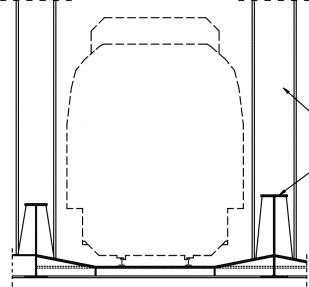
\includegraphics[width=5cm]{skryptkierownik-img/skrajnia.jpg}
	\caption{Przykładowa skrajnia taboru}
\end{marginfigure}
\textbf{Skrajnia taboru} - zarys figury płaskiej, stanowiący podstawę do określania największych dopuszczalnych wymiarów taboru w przekroju poprzecznym.

\textbf{Skrajnia ładunkowa} - zarys figury płaskiej, stanowiący podstawę do określania największych dopuszczalnych wymiarów ładunku spoczywającego na wagonie – pionowych licząc od górnej powierzchni główki szyny oraz poziomych licząc od osi toru.

Skrajnie dzieli się na krajową (ruchu wewnętrznego) i międzynarodową (wszystkie rodzaje pojazdów szynowych z wyjątkiem elektrycznych pojazdów trakcyjnych).

\textbf{Przesyłka nadzwyczajna} - to takie rzeczy lub pojazdy, których przewóz może powodować trudności w przewozie koleją i wymaga zachowania szczególnych warunków techniczno-ruchowych ze względu na: 

\begin{enumerate}
	\item kształt, rozmiary lub masę,
	\item sposób załadowania, rozmieszczenia i zabezpieczenia na wagonie,
	\item użyte środki przewozowe,
	\item drogę przewozu.
\end{enumerate}

Przesyłkę nadzwyczajną w komunikacji krajowej stanowią:

\begin{enumerate}
	\item rzeczy:
	\begin{enumerate}
		\item \textbf{przekraczające} określoną \textbf{skrajnię} ładunkową lub załadowane z przekroczeniem tej skrajni \textit{(szerokość lub wysokość ładunku po umieszczeniu na wagonie, jest większa niż wymiary skrajni ładunkowej)},
		\item wymagające specjalistycznego wagonu, urządzeń, zabezpieczenia bądź szczególnej organizacji przewozu ze względu na położenie środka ciężkości lub inne przyczyny związane z bezpieczeństwem przewozu,
		\item wymagające przewozu w wagonach z zagłębioną podłogą,
		\item o masie jednej sztuki \textbf{ponad 60 t},
		\item powodujące obciążenie na oś wagonu lub metr bieżący toru większe od dopuszczalnego choćby w części drogi przewozu,
		\item wymagające załadowania co najmniej na dwa wagony z ławami pokrętnymi, nie połączone ze sobą sprzęgami wagonowymi lub wagonem pośrednim,
		\item szyny, pręty stalowe do zbrojenia betonu oraz metale giętkie o długości \textbf{ponad 36 m}, ładowane na co najmniej dwa wagony bez ław pokrętnych,
	\end{enumerate}
	\item pojazd kolejowy toczący się na własnych kołach będący sam przedmiotem umowy przewozu lub załadowany przesyłkami:
	\begin{enumerate}
		\item \textbf{ bez znaków RIV, TEN lub RIC}
		\item bez znaków MC,
		\item \textbf{bez świadectwa dopuszczenia} do eksploatacji wydanego przez właściwy organ,
		\item specjalistyczne pojazdy kolejowe np. dźwigi, maszyny torowe i drogowe. Wyjątek stanowią pojazdy kolejowe do wykonywania przewozów technologicznych oraz wieloczynnościowe i ciężkie maszyny do robót budowlanych Zarządcy. Przewozy te realizowane są na podstawie oddzielnych regulaminów opracowanych przez właściwe jednostki Zarządcy, użytkujące te pojazdy,
		\item o średnicy kół \textbf{mniejszej niż 840 mm}, w tym również oznaczony znakami RIV, TEN, RIC lub MC
		\item o przekroczonej skrajni taboru
	\end{enumerate}
\end{enumerate}

Decyzję o zgodzie na przewóz przesyłki nadzwyczajnej podejmuje Zarządca infrastruktury na wniosek Przewoźnika.

\chapter{Ogólne zasady przewozu przesyłek niebezpiecznych}

Zasady przewozu towarów niebezpiecznych określa instrukcja Ir-16

\textbf{Numer UN}– międzynarodowy czterocyfrowy numer towaru niebezpiecznego.

\textbf{RID} – Regulamin międzynarodowego przewozu kolejami towarów niebezpiecznych.
\marginnote{Règlement concernant le transport international ferroviaire des marchandises dangereuses - załącznik do umowy o Międzynarodowej Kolejowej Komunikacji Towarowej (SMGS)}

\textbf{Towary niebezpieczne (TN)} – materiały i przedmioty, których przewóz transportem kolejowym jest zabroniony, albo
dopuszczony na ściśle określonych warunkach, zawartych w przepisach RID

Towary niebezpieczne stanowią materiały i przedmioty, które ze względu na właściwości fizyczne, chemiczne lub biologiczne, stwarzają potencjalne zagrożenie bezpieczeństwa w przypadku niewłaściwego obchodzenia się z nimi w czasie przewozu lub w przypadkach zaistnienia wydarzenia, mogące powodować śmierć, zagrożenie zdrowia, zniszczenie środowiska naturalnego lub dóbr materialnych.

\textbf{Towary niebezpieczne wysokiego ryzyka TWR} -  jest to grupa towarów wyodrębniona z towarów niebezpiecznych, które użyte niezgodnie ze swoim przeznaczeniem, tj. do celów terrorystycznych mogą spowodować poważne skutki, takie jak liczne ofiary, masowe zniszczenia lub szczególnie w przypadku klasy 7, masowe zakłócenia społeczno – gospodarcze.

Oznakowanie przesyłek niebezpiecznych:
\begin{marginfigure}
	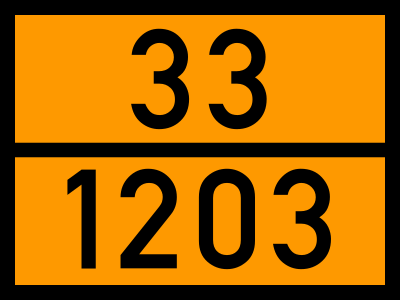
\includegraphics[width=5cm]{skryptkierownik-img/tablica-adr.png}
	\caption{Tablica z symbolami niebezpieczeństwa i substancji, źródło: Wikipedia}
	\label{fig:adr}
\end{marginfigure}	
Na każdej ścianie bocznej wagonu, cysterny, kontenera przewożącego towary niebezpieczne musi być umieszczona \textbf{tablica pomarańczowa}, o wymiarach 40x30 cm, z czarną obwódką. 

W górnej części tablicy znajduje się numer zagrożenia.

W dolnej części znajduje się numer UN.

Jeżeli zagrożenie stwarzane przez dany materiał może być wystarczająco określone jedną cyfrą, wówczas po tej cyfrze stawia się zero.

Podwojenie pewnej cyfry wskazuje na nasilenie odpowiedniego zagrożenia.

Jeżeli numer zagrożenia jest poprzedzony literą „X” oznacza to, że materiał niebezpiecznie reaguje z wodą

Obowiązek umieszczenia tablicy pomarańczowej dotyczy również przewozu próżnych nieoczyszczonych, nieodkażonych oraz nieodgazowanych jednostek transportowych po materiałach niebezpiecznych.
\begin{marginfigure}
	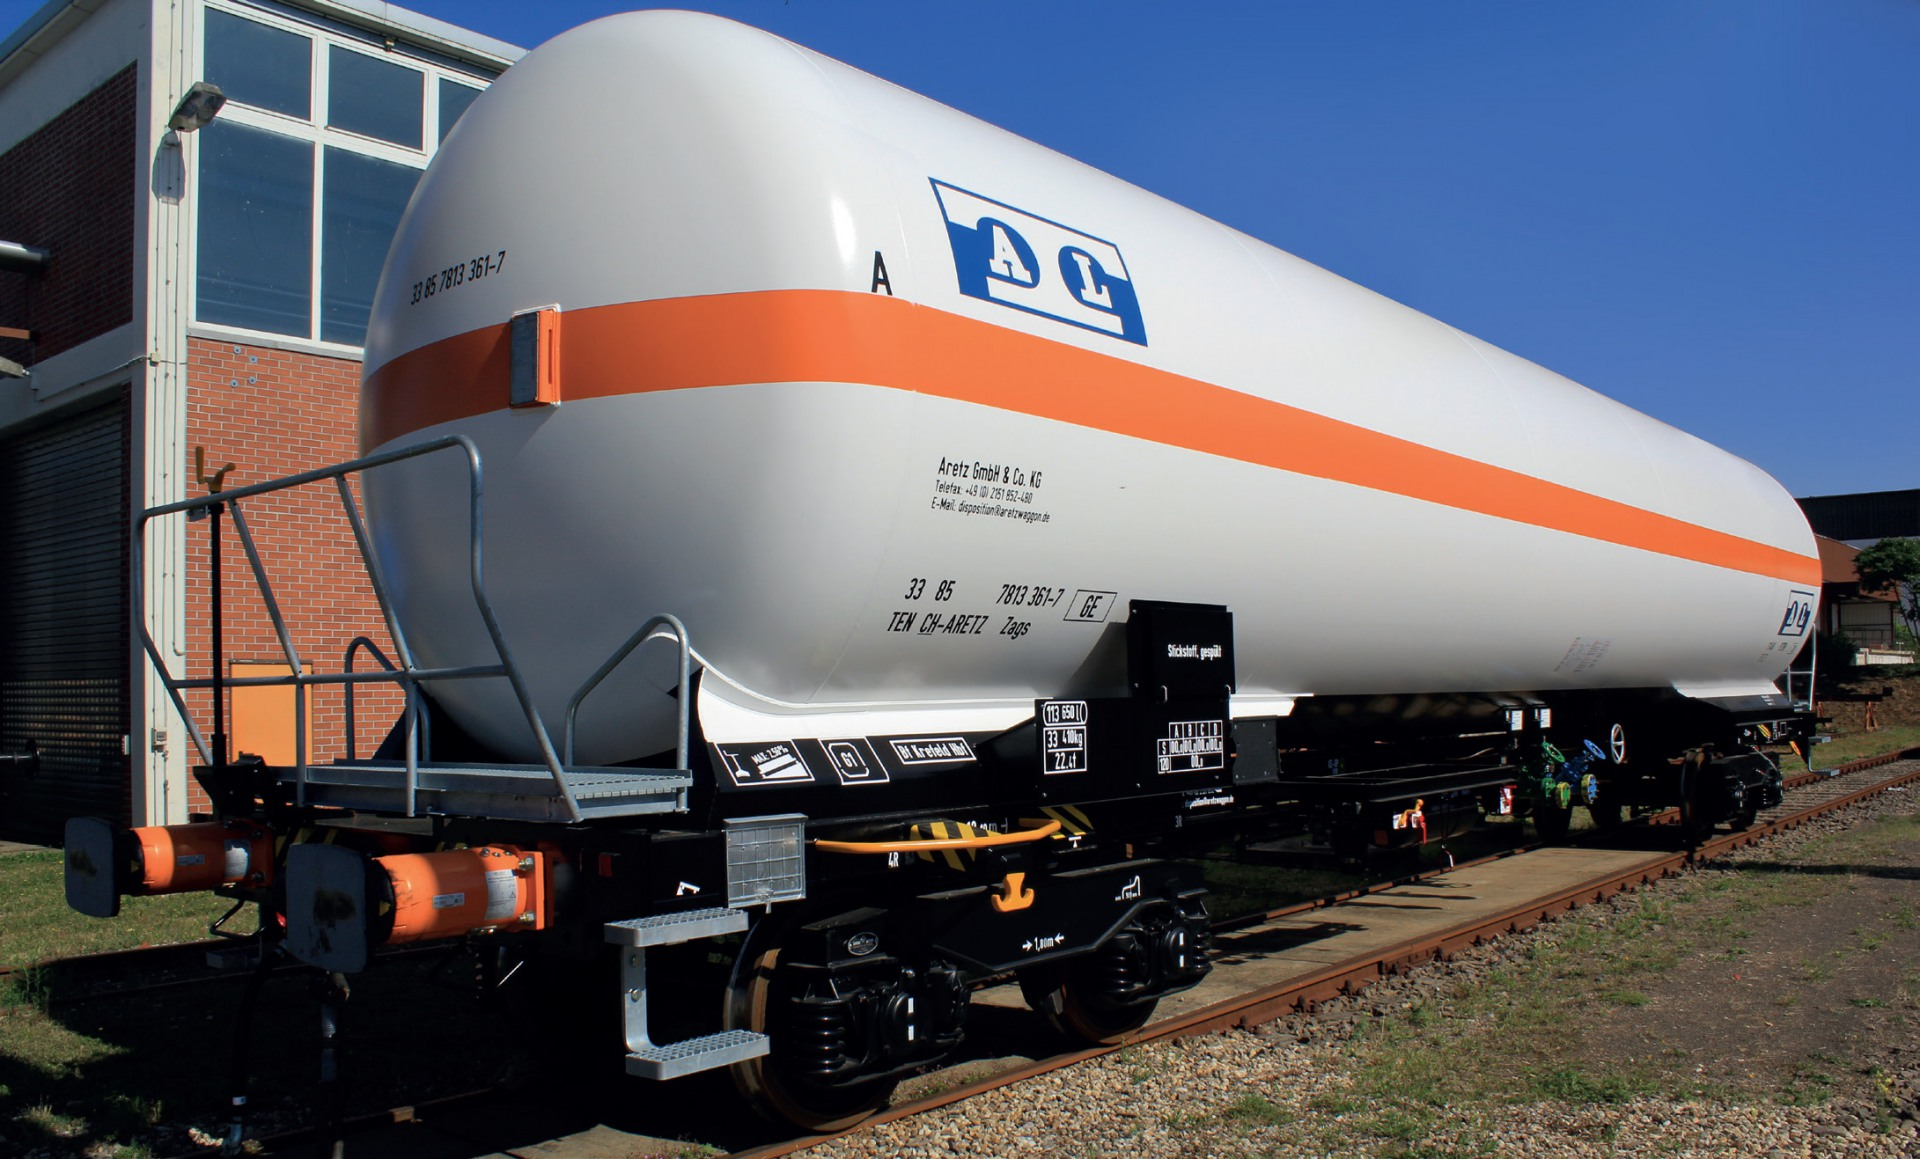
\includegraphics[width=5cm]{skryptkierownik-img/cysterna-rid.jpg}
	\caption{Cysterna do przewozu gazów, za: http://chemet.com.pl}
	\label{fig:cysterna}
\end{marginfigure}
\textbf{Pas} o szerokości ok. 30 cm\textbf{ koloru pomarańczowego} nieodblaskowego na cysternach przeznaczonych do przewozu gazów skroplonych, skroplonych schłodzonych lub rozpuszczonych. Wagony “szerokotorowe” mogą mieć pasy innego koloru dla przewozu specyficznych substancji.

\textbf{Nalepki ostrzegawcze}, umieszczane na opakowaniach, pojemnikach, kontenerach, wagonach, cysternach. Nalepka musi mieć kształ rombu, o wymiarach conajmniej 100 mm dla opakowań i conajmniej 250 mm dla wagonów. Wzory i kolory nalepek
związane są z klasą niebezpieczeństwa, opisane są w części 5 RID.


\chapter{Budowa taboru pasażerskiego}
	\section{Wózek}

Wózki służą do przeniesienia ruchu obrotowego kół na pudło, oraz ustabilizowanie tego ruchu. Pierwsze konstrukcje pojazdów kolejowych posiadały wagony dwuosiowe, bez wózków, z mocowaniem maźnicy zestawu kołowego bezpośrednio do ostoji wagonu. Obecnie większość wagonów wyposażona jest w dwuosiowe wózki które lepiej wpisują się łuki toru. Niektóre lokomotywy, oraz tabor specjalistyczny wyposażone są w wózki trzy- lub wielo-osiowe. Najbardziej rozpowszechnionym typem konstrukcji jest rama skrzynkowa do której montowane są pozostałe elementy wózka.

Wyróżnia się wózki toczne (nie posiadające napędu – wagonowe) i napędowe. Wózki napędowe w lokomotywach elektrycznych i spalinowych z przekładnią elektryczną mają zabudowane silniki(zwykle – 1 silnik na 1 oś). Istnieją (rzadkie) przykłady wózków napędowych bez silników, w których następuje jedynie zamiana ruchu obrotowego wału dostarczającego moc z silnika umieszczonego w pudle lokomotywy na ruch obrotowy kół za pomocą przekładni (rozwiązanie stosowane w spalinowozach z przekładnią mechaniczną). Istnieją też wózki, w których niektóre osie są napędowe, a niektóre toczne (np. lokomotywy spalinowe).

W wózku zabudowane są elementy zapewniające usprężynowanie pojazdu szynowego. Pojazdy służące do przewozu podróżnych cechują się wyposażeniem w dwa stopnie usprężynowania. Dawniej najczęściej stosowane były sprężyny piórowe, obecnie sprężyny śrubowe lub sprężyny metalowo-gumowe, zaś w drugim stopniu elementy pneumatyczne (poduszki). Obok sprężyn w wózkach zamocowane są tłumiki drgań i – w pojazdach dużej
szybkości – tłumiki wężykowania. 
	\begin{figure*}
		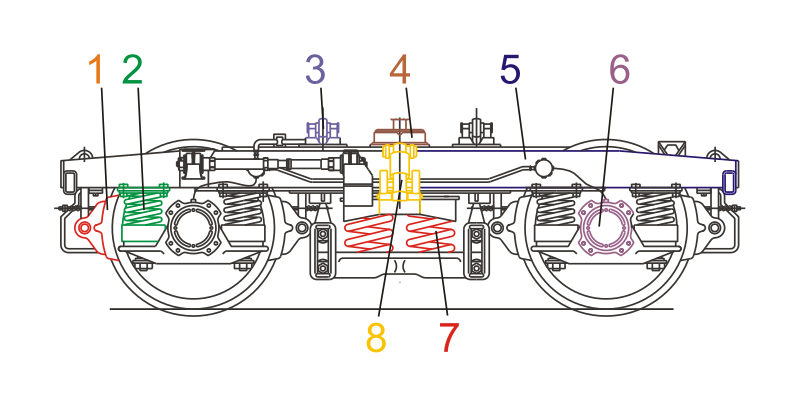
\includegraphics[width=15cm]{skryptkierownik-img/skryptkierownik-img027.png}
		\caption{Elementy budowy wózka, źródło: Wikipedia}
		\label{fig:wozek}
	\end{figure*}

\begin{enumerate}
	\item Klocek hamulcowy
	\item Pierwszy stopień usprężynowania
	\item Podparcia boczne
	\item Czop skrętu
	\item Rama wózka
	\item Maźnica
	\item Drugi stopień usprężynowania
	\item Tłumik drugiego stopnia usprężynowania
\end{enumerate}


\textbf{Pierwszy stopień usprężynowania} tworzy filtr mechaniczny tłumiący i amortyzujący drgania przenoszone z zestawu kołowego na ramę wózka. Elementami sprężystymi w tym rozwiązaniu są w starszych pojazdach sprężyny stalowe piórowe (resory), a w nowszych konstrukcjach sprężyny śrubowe naciskowe (pojedyncze lub wielokrotne), sprężyny gumowe lub sprężyny metalowo - gumowe. 

\textbf{Drugi stopień usprężynowania} tworzy filtr mechaniczny tłumiący i amortyzujący drgania przenoszone z wózka na nadwozie. Elementami sprężystymi w tym rozwiązaniu mogą być sprężyny śrubowe naciskowe lub dwufunkcyjne, sprężyny pneumatyczne, sprężyny metalowo - gumowe lub czasem sprężyny gumowe. 

Rodzaje sprężyn:
\begin{itemize}
	\item Sprężyny stalowe piórowe (\textbf{resory}) składają się z zespołu płaskich sprężyn zwanych piórami, które w części środkowej ujęte są opaską z zaciśniętym klinem. Pióra układane są na sobie w malejącej długości.
	\item \textbf{Sprężyny śrubowe} walcowe to odpowiednio nawinięte na gorąco pręty o przekroju kołowym. Sprężyny takie mogą być prawo lub lewoskrętne w zależności od kierunku ich nawijania. 
	W zależności od konstrukcji pojazdu mogą one pracować w wersji pojedynczej lub wielokrotnej. Wielokrotność polega na zastosowaniu współosiowo zamontowanych sprężyn przeciwnie skręconych (jedna sprężyna w drugiej). 
	Sprężyny śrubowe dzielą się na: sprężyny naciskowe, przenoszące tylko ruchy wzdłuż ich osi (stosowane w I i II st. usprężynowania) oraz sprężyny dwufunkcyjne typu \textbf{„flexicoil”}, czyli w tłumaczeniu „giętka spirala” przenoszące zarówno ruchy wzdłuż ich osi jak również ruchy poprzeczne (stosowane tylko w II st. usprężynowania). 
	Sprężyny dwufunkcyjne z jednej strony osadza się w gniazdach na podłużnicach ramy wózka, a z drugiej strony wspiera się na nich nadwozie. Ponieważ ten typ sprężyn przenosi zarówno ruchy pionowe jak i poziome nie ma potrzeby stosowania pośrednich elementów oparć nadwozia takich jak np. belek bujakowych, czy skrętowych, które umożliwiają realizację ruchów wózka w płaszczyźnie poziomej (obrotów), gdyż możliwość tych ruchów zapewnia już praca tych sprężyn w płaszczyźnie poziomej.
	\item sprężyny gumowe występują w postaci płyt płaskich lub kątowych, krążków, pierścieni stożkowych lub cylindrycznych. Mają dużą zdolność tłumienia drgań o wysokiej częstotliwości oraz dużą pojemność energetyczną względem masy.
	\item \textbf{sprężyny metalowo - gumowe} to elastyczne bloki w których skład wchodzi guma (sprężyna gumowa) odpowiednio zwulkanizowana zwulkanizowana z elementami metalowymi. Wulkanizacja w tym przypadku polega na trwałym powleczeniu (sklejeniu) gumą elementów metalowych. 
	W I stopniu usprężynowania najczęściej stosuje się sprężyny metalowo – gumowe typu pierścieniowego lub klinowego. 
	W tych pierwszych pomiędzy pierścieniami gumowymi znajdują się pasy gumy natomiast środkiem tego zespołu biegnie kolumna prowadząca zestaw kołowy. W rozwiązaniu klinowym, powszechnie stosowanym w nowych pojazdach trakcyjnych, sprężyna składa się z dwóch pakietów kątowych elementów gumowych przedzielonych kątowymi blaszkami.  
	\item  \textbf{sprężyny pneumatyczne} występują w wersjach membranowych lub półtoriodalnych. 
	W taborze pasażerskim najczęściej stosuje się sprężyny półtoriodalne - nie wymagają one stosowania belek skrętowych, gdyż mają właściwości umożliwiające dużą odkształcalność poprzeczną. Sprężyny półtoriodalne oparte są więc bezpośrednio na podłużnicach (belkach ostojnicowych) ramy wózka, a na nich spoczywa nadwozie pojazdu. Sprężyna pneumatyczna składa się z płyty mocującej, pierścienia, powłoki gumowej zwanej miechem sprężyny pneumatycznej wypełnionej sprężonym powietrzem oraz sprężyny dodatkowej. Sprężyna dodatkowa pełni funkcję awaryjną - w przypadku ubytku powietrza w miechu przejmuje obciążenia i umożliwia kontynuowanie jazdy z obniżoną prędkością. Usprężynowanie pneumatyczne wymaga układu zasilania pneumatycznego sprężonym powietrzem i sterowania. W układzie pneumatyki znajduje się zawór ważący, który utrzymuje stałą wysokość sprężyny dostosowując ciśnienie w miechu pneumatycznym do aktualnego obciążenia, reagując na zmiany ugięcia. 
	Sprężyny pneumatyczne naprzeciwległe są połączone pneumatycznie poprzez zawór wyrównawczy, który wyrównuje ciśnienia między sprężynami na wózku. W przypadku awarii jednego z miechów zawór ten wypuszcza też powietrze z miechu sprawnego, tak aby pudło z obydwu stron wparte było na sprężynie dodatkowej (awaryjnej) co zapewni wyrównanie nacisków nadwozia na wózek. 
	\end{itemize}

\textbf{Maźnica} zwana też łożyskiem głównym to element w którego skład wchodzą łożyska toczne (rzadziej ślizgowe) osadzone na czopach łożyskowych osi oraz kadłub (korpus) maźnicy, w którym te łożyska są osadzone. Kształt kadłuba maźnicy jest zależny oraz sposobu prowadzenia zestawu kołowego względem ramy wózka i metody mocowania odsprężynowania pierwszego stopnia.

Podział metod prowadzenia zestawu kołowego:
\begin{itemize}
\item \textbf{prowadzenie sztywne} 
Pierwszym opracowanym na początku istnienia kolei sposobem było sztywne prowadzenie zestawów kołowych do ramy w wyniku czego nie były one usprężynowane.
\begin{marginfigure}
	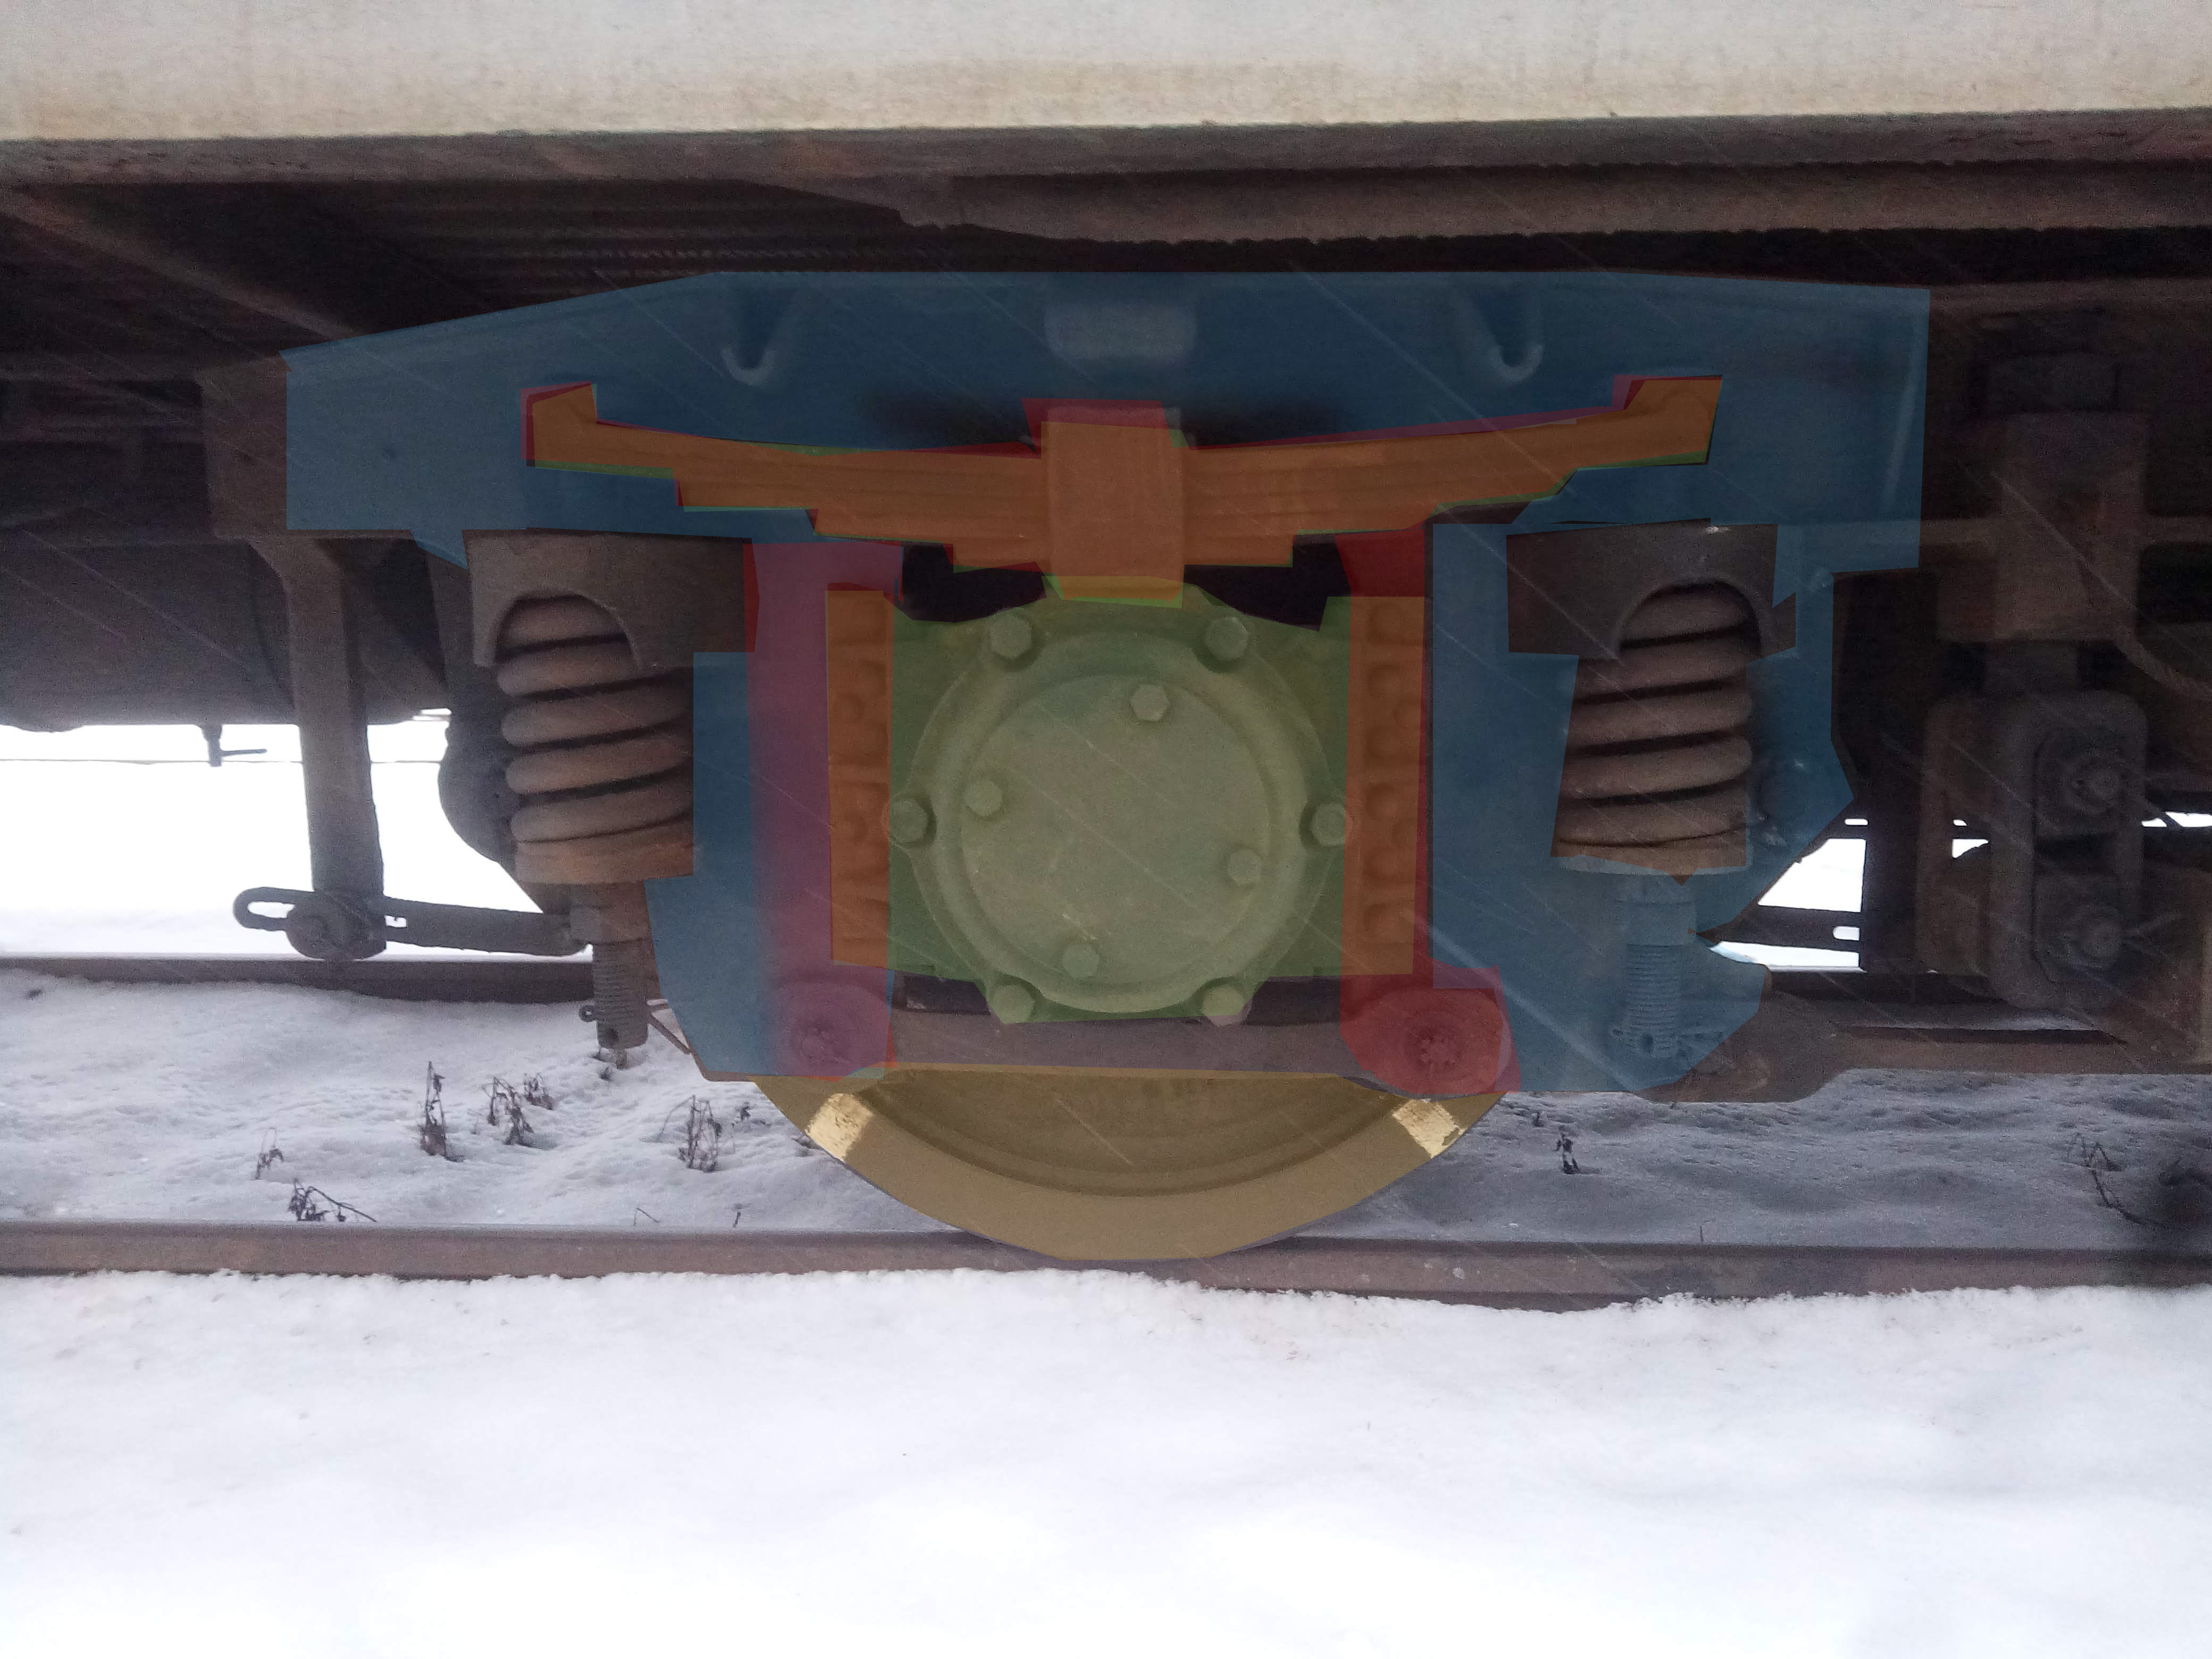
\includegraphics[width=5cm]{skryptkierownik-img/prowadzenie-zestawu-widlowe.jpg}
	\caption{Prowadzenie widłowe. Kolorem niebieskim oznaczona rama wózka.}
\end{marginfigure}
\item \textbf{prowadzenie widłowe} za pośrednictwem tak zwanych wideł maźniczych. Kadłub maźnicy posiada pionowe ścianki ze ślizgami (najczęściej miedzianymi). Ślizgi te te współpracują z wykładzinami wideł maźniczych ramy, które wykonane są ze stali. Prowadzenie widłowe może być jednostronne, dwustronne lub kątowe. 
\begin{marginfigure}
	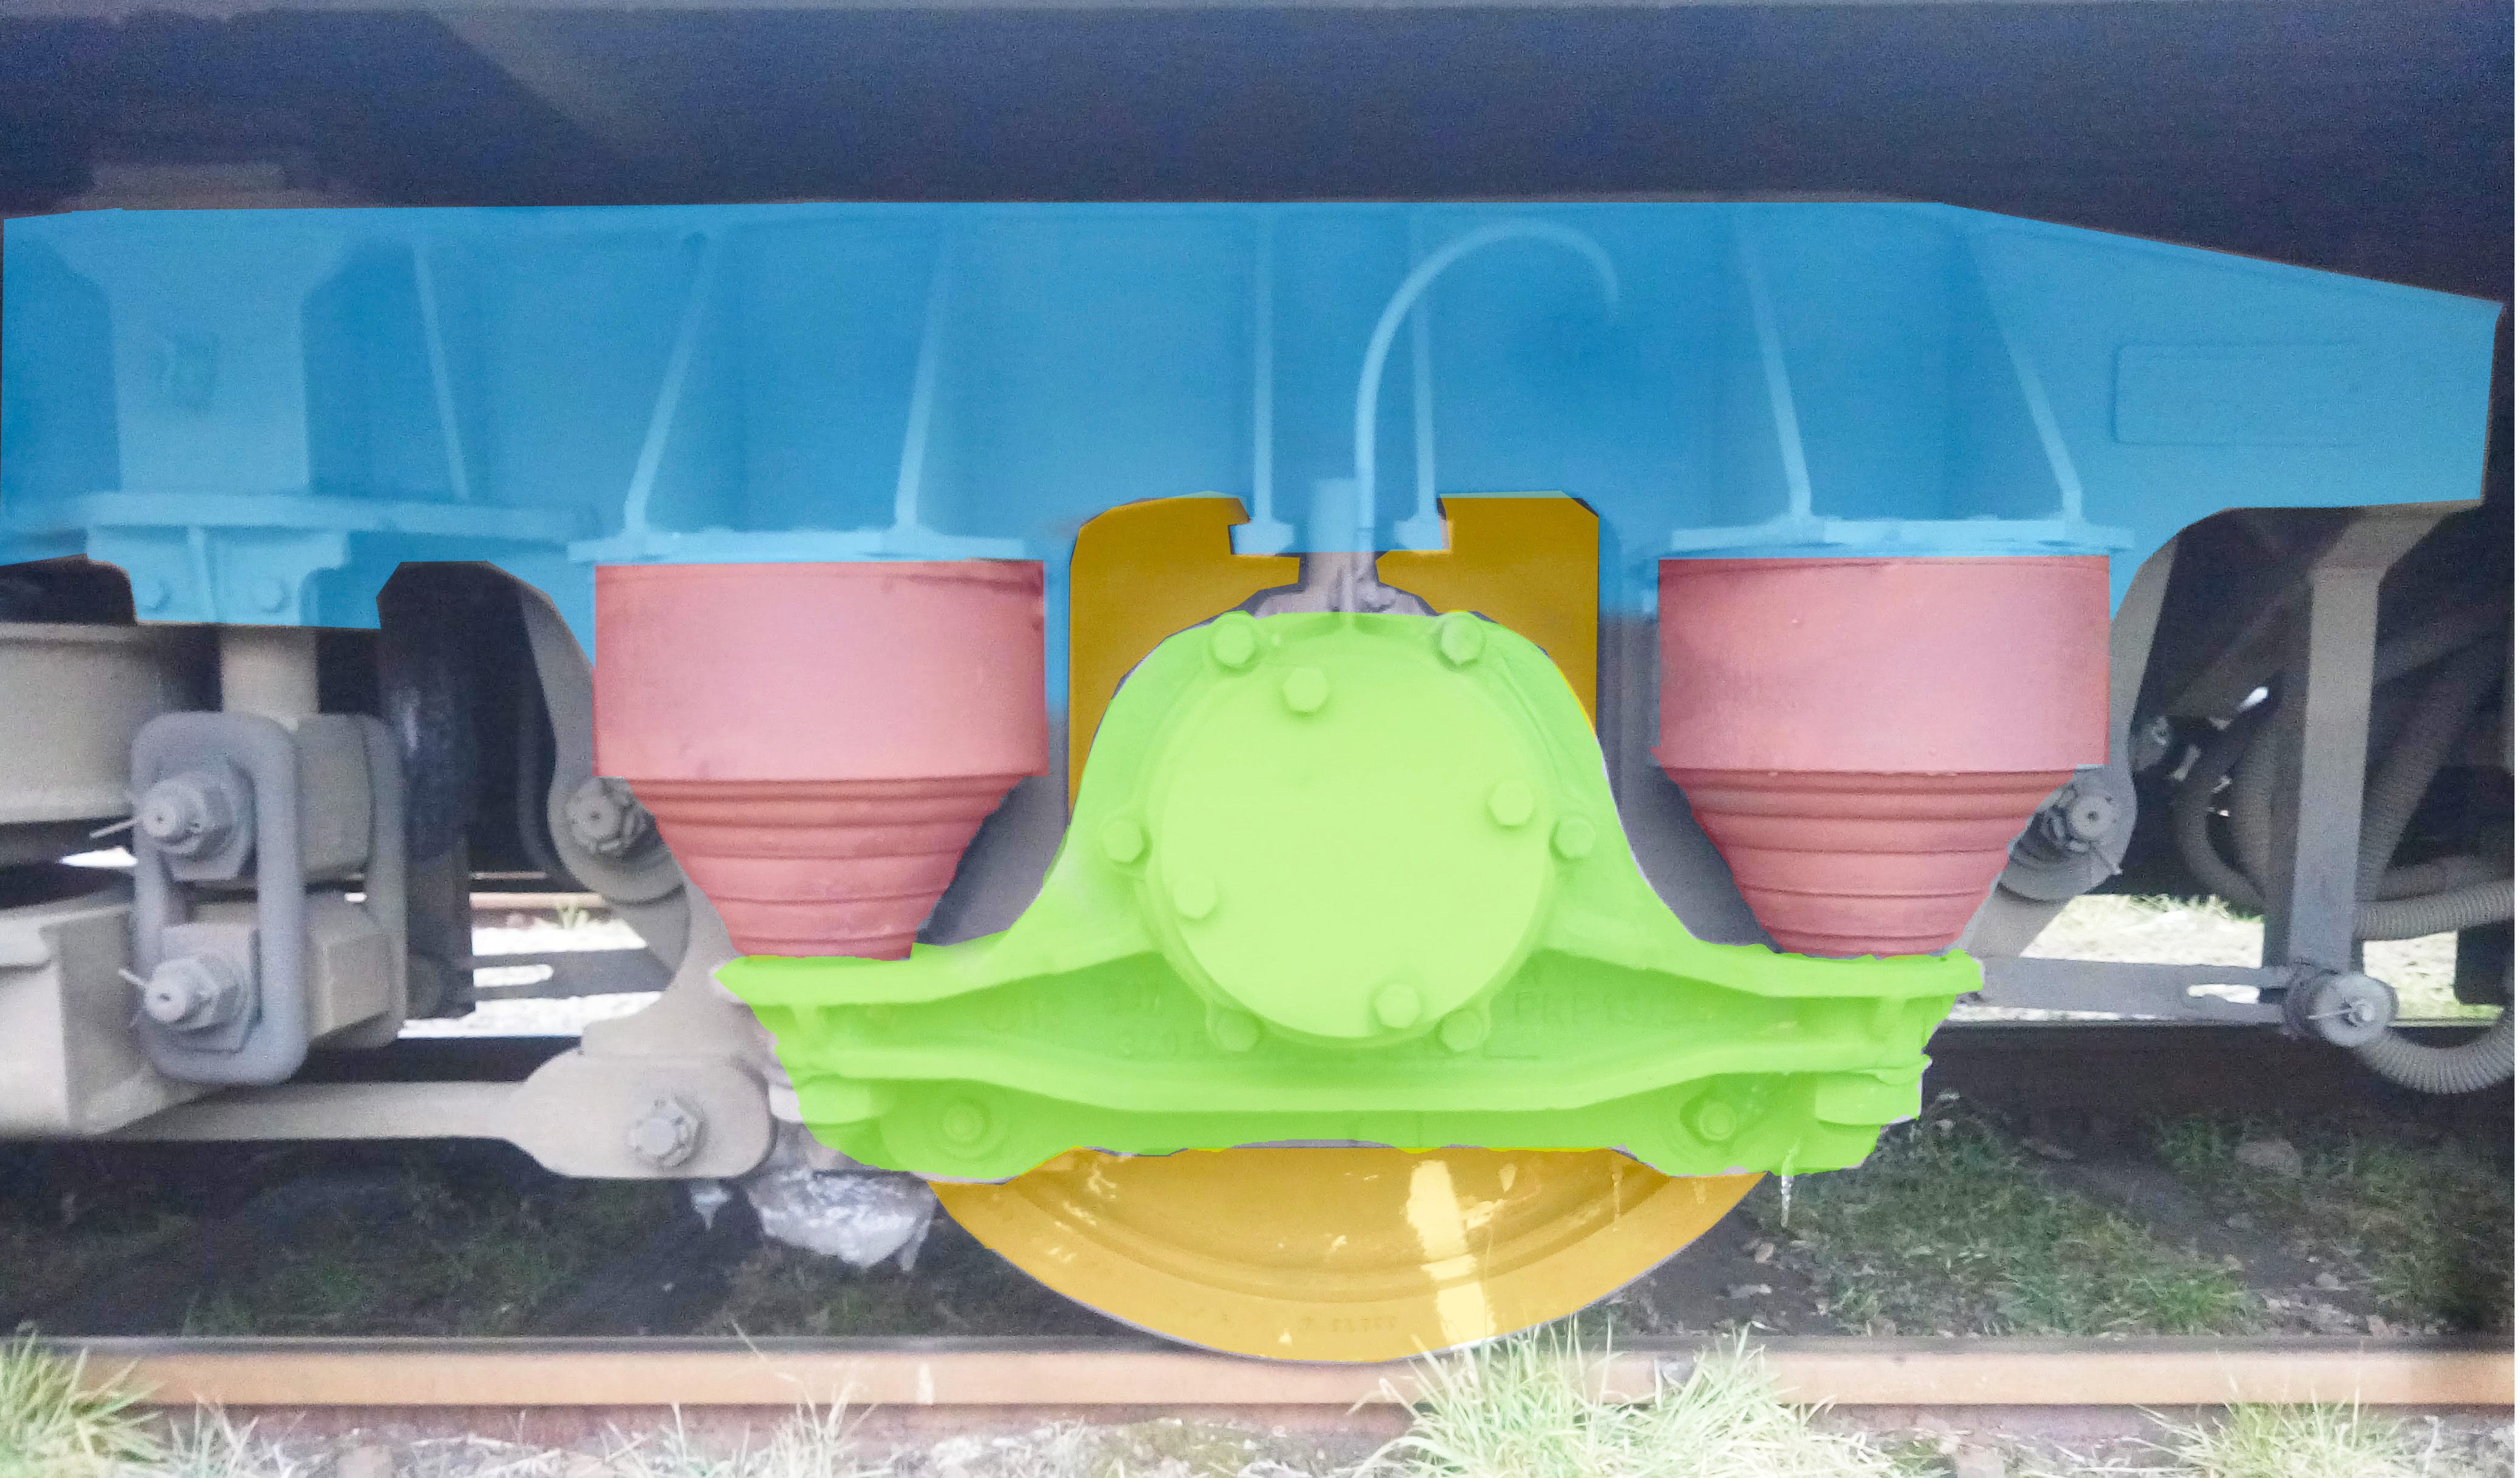
\includegraphics[width=5cm]{skryptkierownik-img/prowadzenie-zestawu-kolumnowe.jpg}
	\caption{Prowadzenie kolumnowe. Kolorem niebieskim oznaczona rama wózka, kolorem pomarańczowym zestaw kołowy, kolorem zielonym korpus maźnicy, zaś kolorem czerwonym kolumny gumowo-metalowe.}
\end{marginfigure} 
\item \textbf{prowadzenie kolumnowe} polegające na zastosowaniu sprężyn stalowych w których znajdują się kolumny prowadzące. Sprężyny i kolumny wsparte są w cylindrycznych gniazdach kadłuba maźnicy, a na ich drugim końcu oparta jest podłużnica ramy wózka (belka ostojnicowa). System ten daje dużą sztywność w płaszczyźnie poziomej, a zużycie cierne elementów prowadzenia jest niewielkie. 
\item \textbf{prowadzenie sprężyste-cięgnowe} (taśmowe) realizowane jest w płaszczyźnie poziomej, a płaskie cięgna sprężyste występują w układzie jedno lub dwustronnym. W prowadzeniu tym nie występuje zużycie ścierne. 
Omówione rozwiązanie występuje głównie w wózkach tocznych, gdyż zastosowane cięgna nie są przystosowane do przenoszenia dużych sił pociągowych i hamulcowych, jakie występują w pojazdach trakcyjnych. Wyjątek stanowią lekkie pojazdy trakcyjne, gdzie siły pociągowe są nieduże.
\begin{marginfigure}
	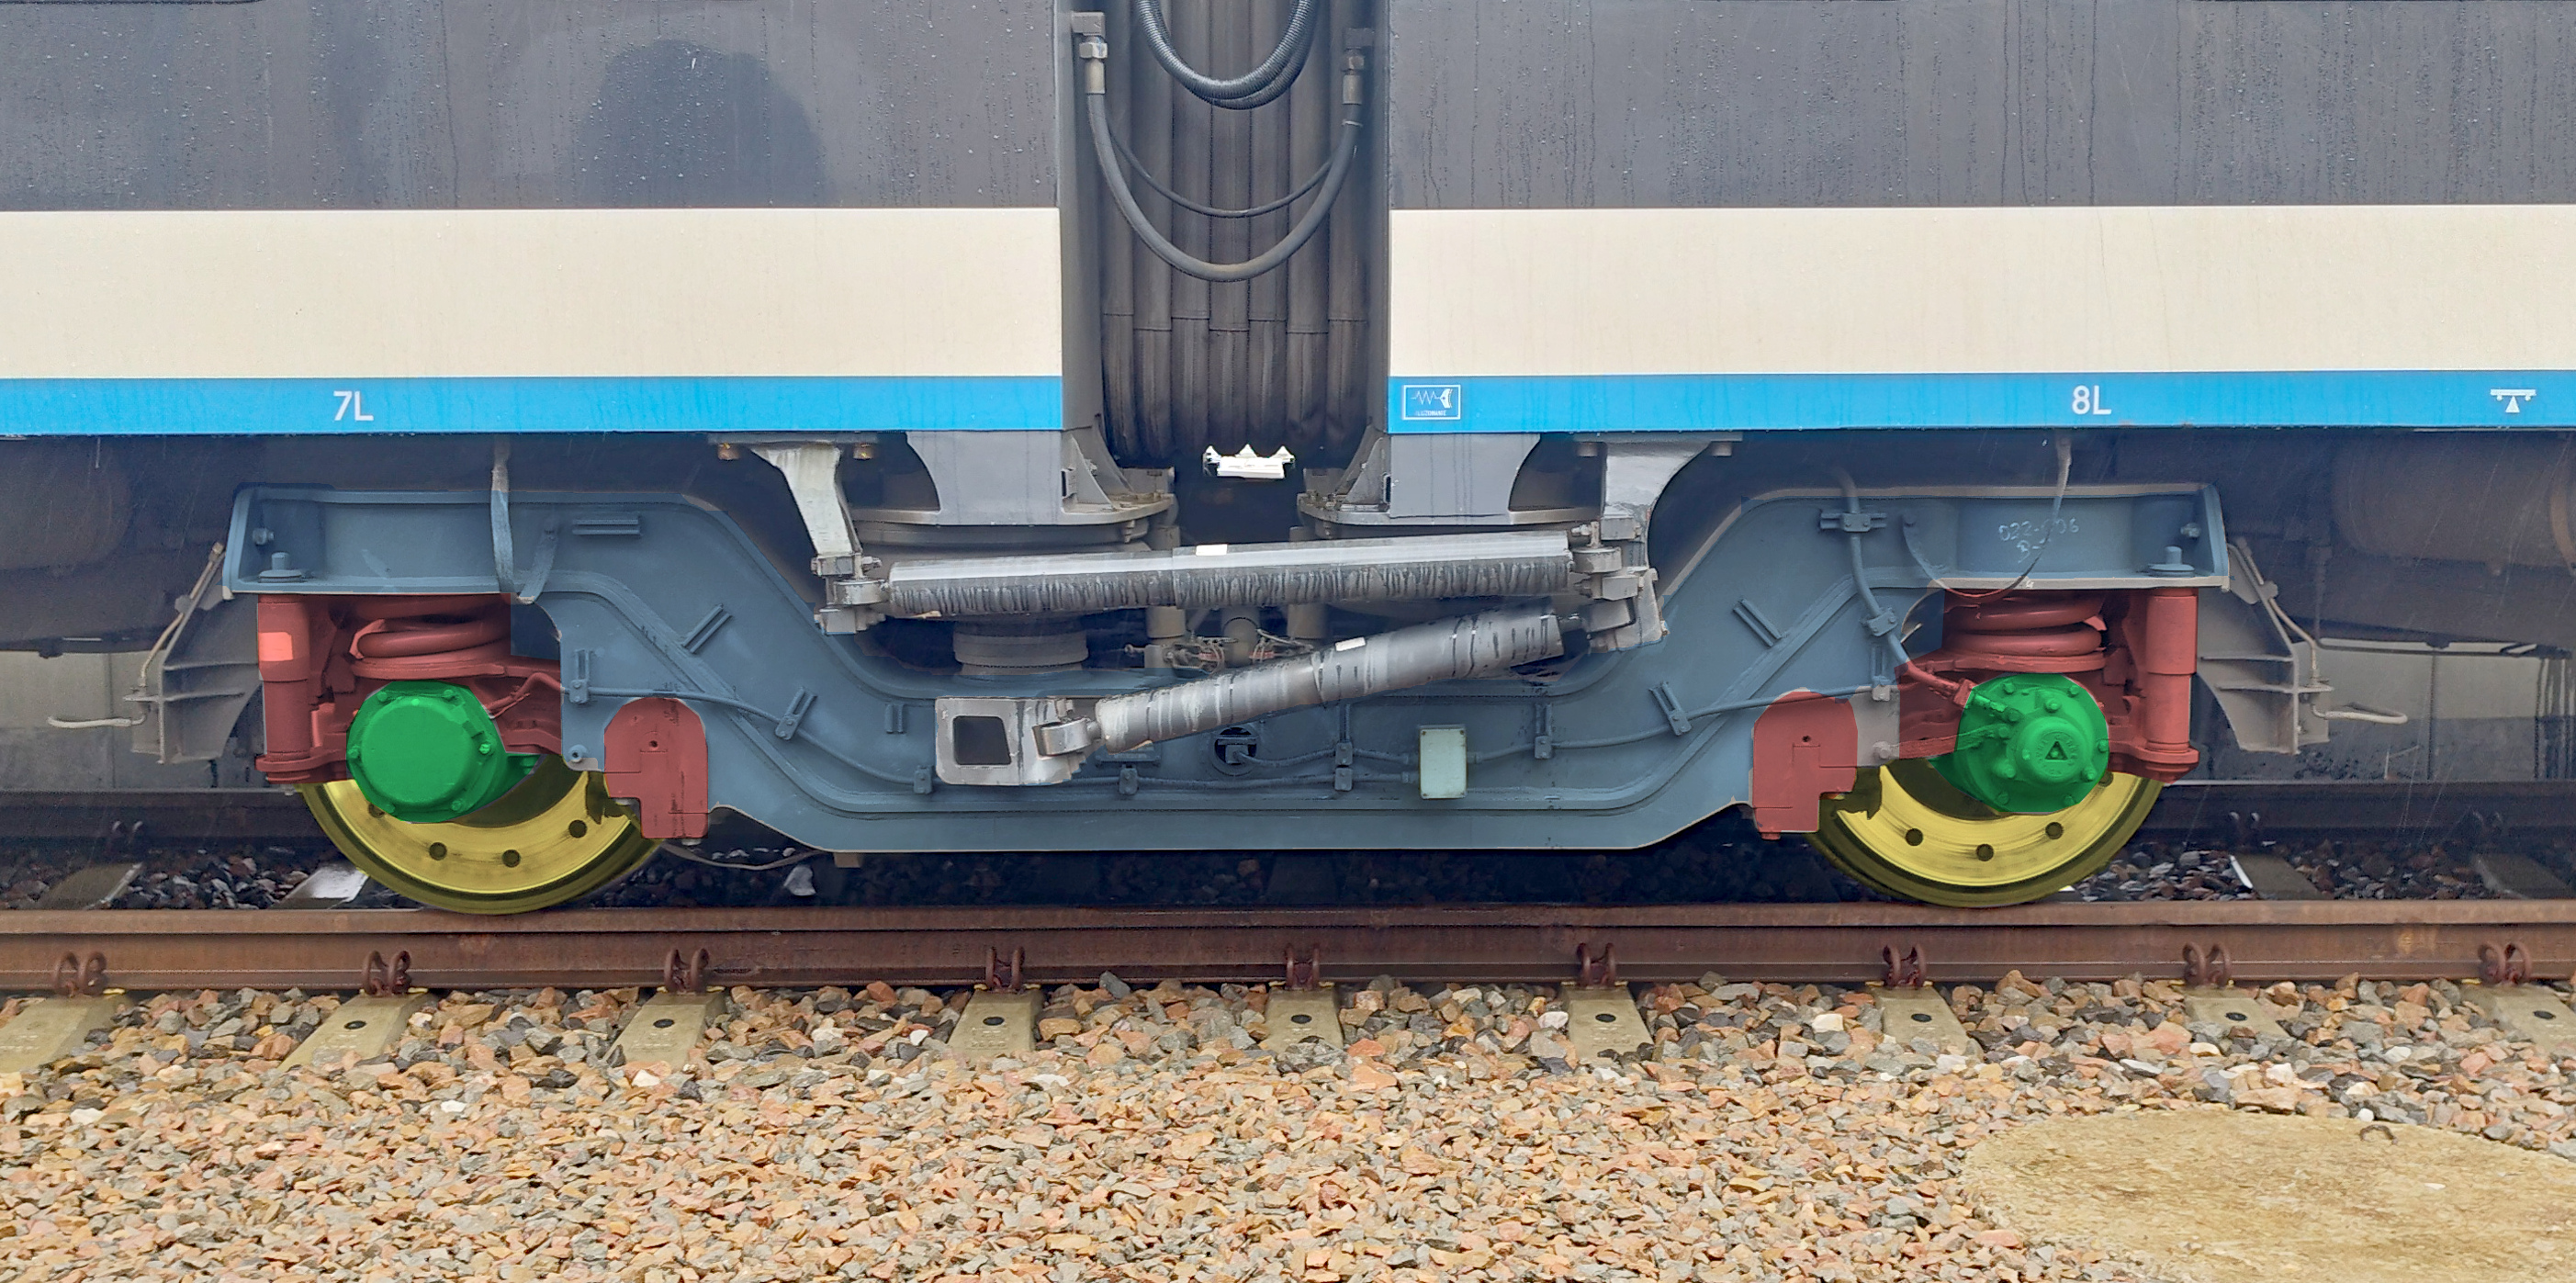
\includegraphics[width=5cm]{skryptkierownik-img/prowadzenie-zestawu-wahaczowe.jpg}
	\caption{Prowadzenie wahaczowe. Kolorem niebieskim oznaczona rama wózka, kolorem pomarańczowym zestaw kołowy. Kolorem czerwonym zaznaczono sprężynę pierwszego stopnia usprężynowania i wahacz.}
\end{marginfigure}
\item \textbf{prowadzenie wahaczowe} - ramię wahacza może być odlane ze staliwa wraz z cylindryczną częścią kadłuba maźnicy lub do niej przyspawane. Zastosowane w tym rozwiązaniu przeguby gumowo-metalowe powodują sprężyste prowadzenie w płaszczyźnie poziomej. Wahacz stanowi jednocześnie prowadzenie w kierunku poprzecznym. 
\end{itemize}

\textbf{Zestaw kołowy} składa się z \underline{osi} oraz \underline{dwóch kół jezdnych} osadzonych na niej w sposób trwały.
Wyróżnia się koła monoblokowe oraz obręczowane. 
Koła obręczowane składają się z \textbf{koła bosego} – piasty (które nabijane jest na podpiaście osi), \textbf{obręczy} i pierścienia \textbf{zaciskowego}. Koło bose może być ramienne lub tarczowe. Te pierwsze wykonywane są zawsze jako staliwne, natomiast koła tarczowe mogą być staliwne lub kute. 
Obręczowanie czyli proces mocowania obręczy na kole bosym polega na podgrzaniu obręczy przez rezystancję prądu elektrycznego do temperatury ponad 250 st. Celsjusza. Zgodnie z zasadą rozkurczania termicznego stali, obręcz zwiększa swoją średnicę w wyniku czego może być nabita na koło bose. W rowku obręczy specjalną walcarką osadza się natomiast pierścień zaciskowy. W procesie stygnięcia obręcz kurczy się i samoczynnie zaciska na kole bosym, a pierścień zaciskowy stanowi dodatkowe zabezpieczenie omówionego połączenia skurczowego.

Na obwodzie koła jezdnego, w miejscu połączenia obręczy z kołem bosym maluje się promieniście białe paski w celu stwierdzenia ewentualnego przesunięcia obręczy. Paski powinny mieć szerokość 30mm, oraz rozmieszczone co 90 stopni na obwodzie koła. \textbf{Poluzowanie} się obręczy, czy też jej \textbf{pęknięcie} jest elementem zagrażającym bezpieczeństwu dlatego konieczne są częste kontrole współpracy tych elementów poprzez uderzanie młotkiem w obręcz i ocenę odgłosu (wykonuje to rewident taboru). 

Koła \textbf{monoblokowe} różnią się od obręczowych tym, że stanowią jedną całość, to znaczy piasta oraz obręcz, zwana w kołach monoblokowych wieńcem, są wykonane z jednego elementu stalowego w związku z czym nie ma możliwości wymiany obręczy po jej zużyciu. Konieczna jest wymiana całego koła. Rozwiązanie to poprawia znacząco bezpieczeństwo jazdy, gdyż nie ma możliwości poluzowania się obręczy. Na obwodzie koła monoblokowego wytłoczony jest rowek wskazujący graniczne zużycie powierzchni tocznej. Rowek ten musi być widoczny w całośći.

Połączenie wózka z pudłem pojazdu zapewnia gniazdo czopa skrętu, zabudowane w górnej części wózka i czop skrętu w pudle. Czop skrętu jest osią obrotu wózka - realizuje jego obroty w płaszczyźnie poziomej zgodnie z kierunkiem torów.  

\section{Urządzenia pociągowo-zderzne}

Urządzenia pociągowo - zderzne w taborze kolejowym służą do mechanicznego połączenia poprzez sprzęgi pojazdów kolejowych ze sobą, przenoszenia sił pociągowych oraz do łagodzenia sił wzdłużnych wynikających z nabiegania pojazdów na siebie podczas jazdy przy jednoczesnym pochłanianiu części energii powstałej na skutek tego nabiegania. Dzięki powyższym możliwe jest uformowanie składu pociągu z zapewnieniem bezpieczeństwa oraz płynnej i komfortowej jazdy.

Pod względem rodzajów urządzeń pociągowo - zderznych rozróżnia się te, gdzie urządzenia sprzęgowe montowane są niezależnie od zderzakowych oraz takie, gdzie stanowią one zintegrowany element.
W pierwszym przypadku na czołach ostoi pojazdów zabudowuje się w osi wzdłużnej pojazdu urządzenie cięgłowe ze sprzęgiem śrubowym, a po obu jego stronach zabudowywane są urządzenia zderzakowe. W drugim przypadku w ostoi zabudowuje się sprzęgi samoczynne, czyli urządzenia w których zintegrowana jest funkcja cięgłowa, sprzęgająca i zderzakowa.

Sprzęgi typu Scharfenberga realizują jednocześnie połączenie mechaniczne, elektryczne i pneumatyczne pojazdów kolejowych. Wykorzystywane są najczęściej do łączenia w trakcję ukrotnioną jednostek trakcyjnych pasażerskich (EZT i SZT).

Zaletą sprzęgów typu Scharfenberga jest ich samoczynność. Umożliwiają one sprzęganie jednostek bez konieczności użycia żadnych dodatkowych narzędzi, urządzeń, ani tym bardziej personelu. Każdy sprzęg omawianego typu składa się z wypustu stożkowego i gniazda dokładnie odpowiadającemu kształtem takiemu wypustowi.
Dojeżdżając z prędkością nie przekraczającą 5km/h jednostką do drugiej jednostki następuje zetknięcie sprzęgów. Łącznik jednego sprzęgu wchodzi w gniazdo drugiego (sercówkę), a łącznik drugiego wchodzi w sercówkę pierwszego. Łączniki samoczynnie zaczepiają się w sercówkach poprzez mechanizm zaczepowy. Ponad głowicą sprzęgu lub po jej bokach znajduje się tak zwana klawiatura, która zapewnia elektryczne połączenie między jednostkami.

W przypadku konieczności sprzęgnięcia pojazdu wyposażonego w sprzęg typu Scharfenberga z pojazdem, który posiada klasyczny sprzęg śrubowy stosuje się specjalne adaptery sprzęgu zwane też półsprzegami, które z jednej strony posiadają
zespół sprzęgu automatycznego, a z drugiej strony zakończone są w sposób umożliwiający założenie na hak cięgłowy.

\section{Odbierak pradu}
Odbieraki prądu pojazdów szynowych to aparaty służące do ruchomego połączenia stykowego sieci trakcyjnej z elektrycznym obwodem głównym pojazdu trakcyjnego. Rozróżnia się odbieraki górne, zwane również pantografami (ang. pantograph), czyli te współpracujące z siecią trakcyjną napowietrzną oraz odbieraki dolne do poboru energii z tak zwanej trzeciej szyny prądowej, która prowadzona jest równolegle do szyn toru na ich poziomie. 
Pantografy są najpopularniejsze w kolejnictwie oraz komunikacji tramwajowej. Odbieraki dolne, używane są głównie na liniach metra oraz szybkich kolei miejskich, gdzie do infrastruktury nie mają dostępu osoby postronne. 

\begin{marginfigure}
	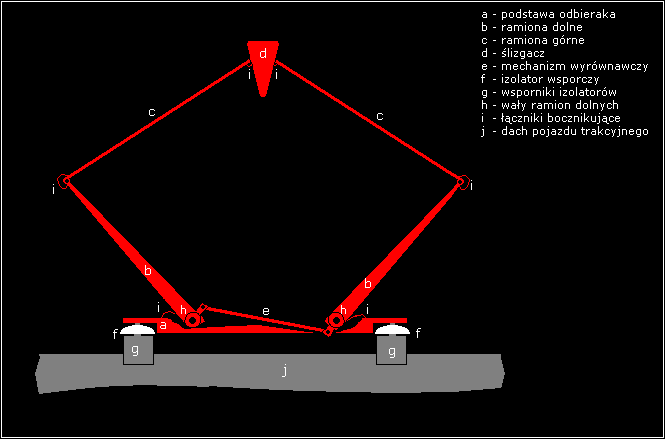
\includegraphics[width=6cm]{skryptkierownik-img/kolodbierakschem1.png}
	\caption{Odbierak o konstrukcji ramy - nożycowej. Źródło: www.transportszynowy.pl}
	\label{fig:pantograf1}
\end{marginfigure}

Odbieraki prądu górne składają się z trzech głównych elementów: podstawy z napędem, ramy przegubowej i ślizgacza. 
\begin{itemize}
	\item \textbf{Podstawa} - to nieruchomy element konstrukcji pantografu, do której przymocowane są części ruchome i układ napędowy. Podstawa jest przymocowana do dachu pojazdu trakcyjnego za pośrednictwem izolatorów wsporczych, izolujących elektrycznie pantograf od pudła pojazdu trakcyjnego. Układ napędowy służy do podnoszenia odbieraka i utrzymywania go w pozycji podniesionej, zapewniając jednocześnie prawidłową siłę docisku do przewodu jezdnego oraz jego opuszczania z zapewnieniem wymaganej siły opuszczającej, a w pozycji dolnej siły utrzymującej go w położeniu złożonym. 

	\item Ruchoma \textbf{rama} przegubowa składa się z układu ramion połączonych przegubowo. Układ ten służy do regulacji pionowej wysokości ślizgacza oraz zapewnia jego docisk na skutek działania układu napędowego. 
	
	
	\item \textbf{Ślizgacz} to część realizująca bezpośredni styk z przewodem jezdnym sieci trakcyjnej. Ślizgacz montowany jest do ramy przegubowej (ramion) elastycznie poprzez zastosowanie np. małego pantografu lub układu elementów sprężystych. Rozróżnia się ślizgacze pojedyncze, w których nakładki ślizgowe powiązane są ze sobą w sposób sztywny oraz ślizgacze bliźniacze w których zastosowane są dwa zestawy nakładek ślizgowych niezależnych lub powiązanych elastycznie. 
\end{itemize}
\begin{marginfigure}
	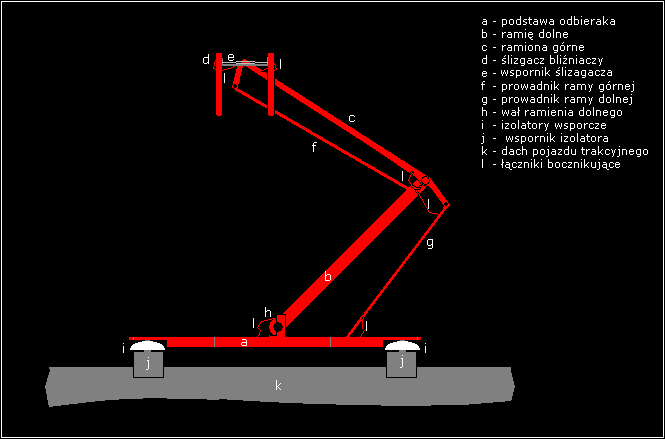
\includegraphics[width=6cm]{skryptkierownik-img/kolodbierakschem2.png}
	\caption{Odbierak o konstrukcji ramy - pantografowej. Źródło: www.transportszynowy.pl}
	\label{fig:pantograf2}
\end{marginfigure}	
Nakładki ślizgowe to elementy bezpośrednio stykające się z przewodem jezdnym. Wykonane są ze sprasowanego grafitu (węgla metalizowanego, węgla twardego). Parametry nakładek muszą być odporne na nagrzewanie i spełniać wymagania dotyczące obciążalności prądowej. W przypadku stosowania nakładek miedzianych ślizgacz pokrywa się warstwą smaru grafitowego, który zmniejsza rezystancję i tarcie, a jednocześnie jest źródłem bardzo widocznych zabrudzeń pojazdów. 
Po zewnętrznych stronach ślizgaczy znajdują się nabieżniki, które służą do wprowadzania przewodu jezdnego dochodzącego z boku na część roboczą ślizgacza. 

Pod względem elektrycznym odbierak prądu musi zapewniać prawidłowy przepływ energii elektrycznej przez swoją konstrukcję. Przegubowa budowa pantografów stwarza szczególnie właśnie w rejonie przegubów miejsca zakłóceń dla toru prądowego biegnącego z przewodu jezdnego, przez ślizgacz, ramę przegubową, do zacisku wyjściowego znajdującego się w ramie podstawy. Z tego powodu na przegubach stosuje się tak zwane łączniki bocznikujące. Są to elementy wykonane z giętkiej linki lub taśmy miedzianej, które poprawiają przepływ energii elektrycznej przez odbierak. Łączniki bocznikujące występują na łączeniach pomiędzy ślizgaczem, a ramionami górnymi, na przegubie ramion górnych z dolnymi oraz pomiędzy ramionami dolnymi, a ramą podstawy. 

Podniesienie odbieraka prądu do pozycji roboczej (styk z przewodem jezdnym) umożliwia pełne uruchomienie pojazdu trakcyjnego dzięki podłączeniu go do zasilania. W pojazdach kolejowych do podnoszenia odbieraków prądu wykorzystywany jest napęd pneumatyczny, znajdujący się w podstawie. Jednak, aby on zadziałał potrzebne jest sprężone powietrze nabite przez sprężarkę. Do uruchomienia sprężarki głównej w pojazdach potrzebne jest napięcie sieciowe, którego przy opuszczonym pantografie w pojeździe nie ma. Z tego też powodu w celu podniesienia odbieraków prądu przy uruchamianiu pojazdu w przypadku braku ciśnienia w zbiorniku głównym, pantografy posiadają niezależną sprężarkę ze zbiornikiem, która zasilana jest z baterii akumulatorów. Najpierw załącza się ją, a po nabiciu przez nią powietrza, maszynista podnosi pantograf. Po zasileniu pojazdu napięciem sieciowym, układ pneumatyczny pantografów zostaje przełączony na zasilanie ze sprężarki głównej (głównego układu pneumatycznego). 

Przewody jezdne sieci trakcyjnej kolejowej zawieszane są na wysokości od minimalnej 4900mm do maksymalnej 6200mm ponad główkę szyny. W takim zakresie wysokości ślizgacz musi mieć zapewniony prawidłowy docisk do przewodu jezdnego.

Jazda z podniesionym tylnym odbierakiem jest najbardziej optymalna, gdyż w przypadku złamania podniesionego odbieraka prądu nie opadnie on na pantograf złożony przez co będzie możliwa jazda awaryjna na pantografie przednim. Poza tym następuje zużycie nakładek ślizgowych tylko jednego slizgacza. Drugi pantograf pełni funkcję rezerwową. 

\section{Warunki techniczne jakim powinien odpowiadać tabor w składzie pociągu}

Wagony które nie posiadają blokady drzwi wejściowych, nie mogą być dopuszczone do ruchu międzynarodowego.

Przestrzeń berneńska (również prostokąt berneński) – wolna przestrzeń przed czołem pojazdu szynowego, w której nie mogą znajdować się żadne części taboru, stanowiąca bezpieczne miejsce dla pracownika spinającego wagony. Przestrzeń ta powinna być wolna od części stałych. W związku z tym wymaganiem części składowe mechanizmu sprzęgającego powinny znajdować się w położeniu bocznym względem jego linii środkowej.

W przestrzeni tej mogą znajdować się kable połączeniowe i węże elastyczne, jak również elastyczne odkształcalne elementy przejść międzywagonowych. Pod zderzakami nie powinny znajdować się żadne urządzenia, które utrudniałyby dostęp do omawianej przestrzeni. 
Części sprzęgów śrubowych, hamulcowych i innych sprzęgów nie mogą zwisać niżej niż \underline{140mm} powyżej główki szyny.

Powierzchnia toczna koła nie może być miejscami wgnieciona, mieć płaskich miejsc i nalepów \textbf{dłuższych} niż \underline{60mm}, oraz o \textbf{głębokości lub wysokości} do \underline{1mm}. Powierzchnia toczna nie może mieć żadnych rys na przejściu z powierzchni tocznej na czołową. Uszkodzenia na powierzchni tocznej (wyłupania, dziury, złuszczenia, odpryski) nie mogą być dłuższe niż 60 mm. W razie powstania wyżej opisanych nalepów hamulec zespolony należy wyłączyć. Wagon okleić nalepkami według wzoru $R^{1}$ („Hamulec niezdatny do użytku”) i \textbf{M} („Do zbadania”), na których należy zaznaczyć : „Nalepy na powierzchni tocznej”.
Koła obręczowane z wytoczonym rowkiem na zewnętrznej powierzchni czołowej obręczy, pokazującym zużycie, są niedozwolone.
W kołach monoblokowych minimalna grubość wieńców kół musi być oznaczona za pomocą \textbf{rowka} wytoczonego na zewnętrznej powierzchni czołowej koła. Rowek musi być stale w całości widoczny.
Obręcze nie mogą mieć żadnego pęknięcia oraz żadnej rysy poprzecznej ani podłużnej. W kole obręczowanym - obręcz nie może być luźna.
Obręcz należy uważać za luźną, jeśli wykazuje co najmniej jedna z niżej wymienionych oznak:

\begin{itemize}
	\item obrót obręczy na kole bosym w płaszczyźnie koła, stwierdzony przez nie pokrywanie się znaków kontrolnych na kole bosym i obręczy.
	\item nieczysty dźwięk przy uderzeniu młotkiem
	\item luźne osadzenie pierścienia zaciskowego,
	\item występowanie rdzy na więcej niż 1/3 obwodu między obręczą a kołem bosym
	\item obręcz nie może wykazywać żadnych śladów bocznego przesunięcia (boczne przesuniecie może zaistnieć tylko wtedy, gdy brak pierścienia zaciskowego, jest luźny, złamany lub widocznie zniekształcony).
	\item pierścień zaciskowy nie może posiadać żadnej rysy. Jeśli dla zabezpieczenia pierścienia zaciskowego przewidziany jest klin zabezpieczający, nie może go brakować.
\end{itemize}

Koło nie może wykazywać żadnych śladów przesunięcia na osi zestawu. Występowanie oleju między osią zestawu kołowego i piastą koła nie jest dowodem, że koło przesunęło się na osi; przesunięcie takie musi być udowodnione.
Piasta koła nie może mieć żadnej rysy. Koło monoblokowe lub tarcza koła nie mogą wykazywać żadnych śladów usuwania usterek spawaniem oraz żadnej rysy.

Oś zestawu kołowego nie może mieć żadnych śladów rys ani śladów naprawiania uszkodzeń przez spawanie, być zgięta, mieć żadnych wytartych miejsc z ostrymi krawędziami, wykazywać żadnych wytartych miejsc o głębokości większej niż 1 mm. Cięgła hamulcowe lub inne części nie mogą trzeć o oś zestawu. Uszkodzone części należy zdemontować lub wysoko umocować tak, aby ich tarcie o oś było niemożliwe. W tym przypadku, a także gdy oś zestawu ma wytarcia mniejsze niż podano wyżej, wagon należy okartkować nalepkami według wzoru \textbf{M} („Do zbadania”), na których należy zaznaczyć „zestaw kołowy”.

W razie podejrzenia termicznego wpływu hamulca na koła monoblokowe objawiające się przez:
\begin{itemize}
	\item świeże ślady spalenia farby na przejściu wieńca w tarczę lub świeże ślady utlenienia wieńca koła lub
	\item nadpalone wstawki hamulcowe lub
	\item uszkodzona powierzchnia toczna z nalepami
\end{itemize}
należy dokonać pomiaru rozstawu kół między wewnętrznymi czołowymi powierzchniami wieńców kół.
 
Łożyska zestawu kołowego nie mogą być tak uszkodzone, aby wyciekał z nich środek smarny lub mógł do ich wnętrza dostawać się kurz i woda. Występy prowadne maźnic muszą w każdym położeniu maźnicy obejmować prowadniki wideł lub odpowiednie części wózków. Łożysko nie może być tak gorące, aby nie można było go dotknąć zewnętrzną powierzchnią dłoni. Łożyska mogą być smarowane i naprawiane przez przedsiębiorstwo kolejowe właściciela. W razie uszkodzenia musi być zawsze wbudowany nowy zestaw kołowy.

Sprężyny śrubowe (spiralne) i piórowe nie mogą być złamane, zaś sprężyny piórowe również przesunięte wzdłuż w opasce o więcej niż 10mm. Wszystkie sprężyny muszą być prawidłowo osadzone w swoich mocowaniach. Tłumiki nie mogą być luźne, oraz posiadać oznak uszkodzeń takich jak wycieki, nieszczelność. wieszaki belek bujakowych i prowadniki zestawów kołowych nie mogą być zgięte , pęknięte, lub złamane,a ich połączenia luźne. Połączenia spawane poprzecznic i podłużnic nie mogą mieć rys. W tych elementch konstrukcyjnych nie mogą również występować żadne nadpęknięcia wychodzące od spoin spawalniczych.
Złamania, uszkodzenia i nadpęknięcia podłużnic, poprzecznic, ram wózków, wsporników belki bujakowej oraz połączeń wózków mogą być naprawiane przez spawanie tylko przez właściciela wagonu.

W każdym wagonie musi być zgodnie z kartą UIC 564-2 przynajmniej jedna gaśnica. W wagonach sypialnych i restauracyjnych muszą być po dwie gaśnice,
Gaśnice muszą być stale zdatne do użytku i dostępne dla podróżnych. 

Wszystkie drzwi wejściowe muszą mieć urządzenia blokujące zapobiegające niezamierzonemu otwarciu drzwi wejściowych w czasie jazdy. Drzwi wagonowe, ich urządzenia prowadne i zamykające oraz elektropneumatyczne urządzenia zamykania drzwi i urządzenia blokowania drzwi nie powinny wykazywać żadnych usterek, które w znacznym stopniu ograniczają użycie wagonu, względnie zagrażają bezpieczeństwu uchu.

\subsection{Oznakowanie i symbole na taborze}

Każdy wagon musi być oznaczony numerem EVN oraz symbolem opisującym cechy techniczne wagonu albo typ i numer serii pojazdu trakcyjnego. Dodatkowo wagon powinien posiadać znaki RIV, RIC, TEN lub MC.

\textbf{Europejski numer pojazdu} (ang. European Vehicle Number, EVN) to numer składający się z 12 cyfr zawierający informacje o charakterystyce technicznej pojazdu kolejowego. 
Numer ten zapisujemy w kilku blokach z których pierwszy (dwucyfrowy) oznacza kod interoperacyjności - przy czym jeśli pierwsza cyfra to 9, jest to pojazd trakcyjny, zaś druga cyfra tego bloku opisuje sposób napędu i konstrukcji (4 oznacza EZT małej prędkości). Kolejne dwie cyfry to kod kraju (Polska to 51), kolejny, jednocyfrowy blok oznacza przeznaczenie pojazdu (cyfra 2 oznacza zespół trakcyjny). W kolejnym bloku opisane są sposób zasilania i moc pojazdu w MW. Pozostałe cyfry oznaczają numer kolejny pojazdu, zaś ostatnia cyfra jest cyfrą samokontroli.

Umowy RIV i RIC zostały zawarte w 1922 r. jako porozumienia międzynarodowe pomiędzy przedsiębiorstwami przewozowymi. Umowa RIV została rozwiązana 1 lipca 2006 r. Jednocześnie za  następcę tej umowy w obrocie międzynarodowym uznać można Ogólną umowę o użytkowaniu wagonów towarowych (GCU, AVV).

Podstawowymi zadaniem ww. umów jest uznawanie za dopuszczone do eksploatacji pojazdów kolejowych przez krajowe organy regulacji rynku kolejowego. Porozumienia te określają warunki, których spełnienie uzależnia możliwość wymiany pojazdów pomiędzy sygnatariuszami porozumienia. Spełnienie wymagań wskazanych w umowach jest stwierdzane poprzez nadanie pojazdom odpowiednio oznaczenia RIV lub RIC.
\begin{marginfigure}
	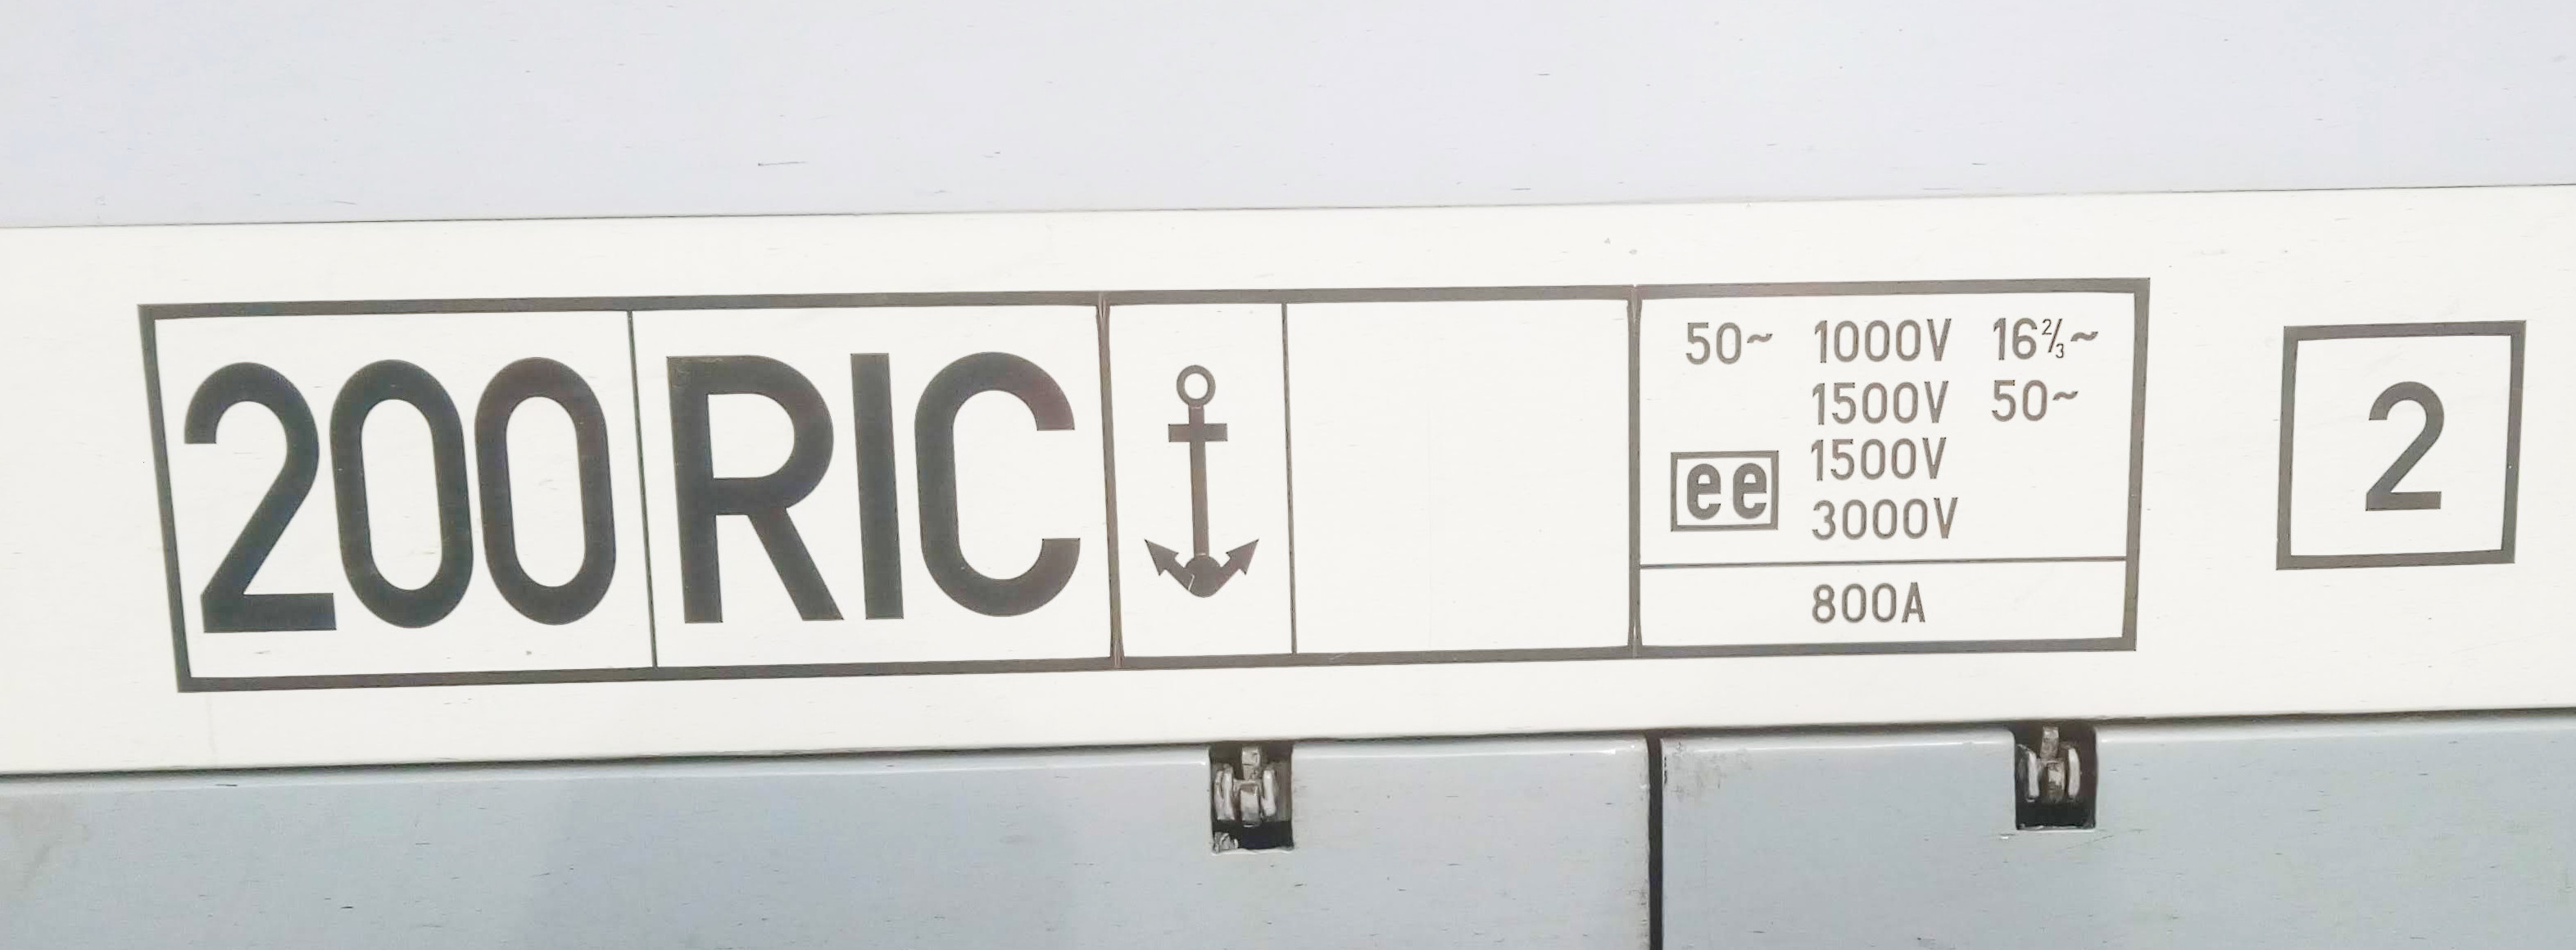
\includegraphics[width=6cm]{skryptkierownik-img/znak-ric.jpg}
	\caption{Znak RIC na wagonie PKP Intercity}
	\label{fig:pantograf2}
\end{marginfigure}

\textbf{RIV} - umowa międzynarodowa Regolamento Internazionale Veicoli. Były to przepisy o wzajemnym użytkowaniu wagonów towarowych w komunikacji międzynarodowej. Zostały zastąpione przez GCU (General Contract of Use for Wagons, czyli ogólna umowa o użytkowaniu wagonów towarowych).

\textbf{RIC} - umowa międzynarodowa Regolamento Internazionale Carozzi. Były to przepisy o wzajemnym użytkowaniu wagonów osobowych i bagażowych w komunikacji międzynarodowej.

\textbf{SMGS} - Umowa o międzynarodowej komunikacji towarowej obowiązująca w krajach Europy wschodniej (kraje dawnego ZSRR), Dalekiego Wschodu (Chiny, Korea, Wietnam, etc.) 

\textbf{Znak MC} - wagon spełniający przepisy PPW - określające normy i wymagania dla przewozów na podstawie umowy SMGS. 


\section{Wyłączanie taboru z eksploatacji}

\textbf{Przeglądy} – zabiegi zapobiegawcze wykonywane na sprawnym technicznie pojeździe w celu sprawdzenia zgodności stanu technicznego pojazdu trakcyjnego z obowiązującymi wymogami bezpieczeństwa ruchu kolejowego i eksploatacyjnymi określonym m.in. w \textbf{Dokumentacji Systemu Utrzymania} (DSU).

\textbf{Naprawy} - czynności mające na celu doprowadzenie wyeksploatowanego (zużytego) lub uszkodzonego pojazdu trakcyjnego wyłączonego z ruchu, jego zespołu, podzespołu, elementu, obwodu lub układu do wymaganego przepisami technicznymi stanu pełnej sprawności wg wymogów (DSU) umożliwiającego dalszą bezpieczną eksploatację.

\textbf{Poziom utrzymania pojazdu kolejowego} – zestawienie czynności utrzymaniowych wykonywanych dla danego pojazdu kolejowego określone zakresem tych prac;

\textbf{Modernizacja pojazdu kolejowego} – prace modyfikacyjne w pojeździe kolejowym, które zmieniają przeznaczenie pojazdu lub poprawiają jego ogólne osiągi techniczne, a w szczególności: zmianę charakterystyki trakcyjnej, prędkości maksymalnej, mocy, zdolności do zasilania w różnych systemach;
Wyłączenie pojazdu trakcyjnego z eksploatacji winno nastąpić gdy pojazd nie spełnia wymagań formalnych lub technicznych i nie zapewnia odpowiedniego poziomu bezpiecznej eksploatacji.

Pojazd kolejowy nalezy wyłączyć z eksploatacji, jeżeli:
\begin{enumerate}
	\item jego świadectwo sprawności technicznej utraciło ważność,
	\item kiedy wymaga wykonania przeglądu poziomu 1,2, lub 3.
	\item w razie dalszej eksploatacji zachodzi uzasadnione prawdopodobieństwo
	przekroczenia dopuszczalnego czasokresu bądź przebiegu do następnego
	przeglądu poziomu utrzymania 1, 2 lub poziomu 3 - zgodnie z obowiązującą
	dla danej serii pojazdu trakcyjnego dokumentacją systemu utrzymania.
	\item wymaga wykonania naprawy okresowej lub bieżącej, awaryjnej, bądź usunięcia
	usterek i innych nieprawidłowości - w szczególności, gdy uczestniczył w zdarzeniu kolejowym, bądź w książce pokładowej pojazdu kolejowego z napędem znajdują się adnotacje o nieprawidłowościach istotnych dla bezpieczeństwa ruchu kolejowego,
	\marginnote{Wszystkie oznaczenia takie jak EVN, masy służbowe, hamujące, oznaczenia nastawienia hamulca, etc. muszą być czytelne.}
	\item znaki i napisy na pojeździe trakcyjnym są nieczytelne lub niezgodne z obowiązującymi przepisami,
	\item pobieżne, zewnętrzne oględziny pojazdu trakcyjnego lub działanie zespołów, podzespołów i elementów mogą wskazywać na uszkodzenia lub inne, istotne nieprawidłowości,
	\item wynika to z wewnętrznych poleceń kierownictwa komórki organizacyjnej Spółki
\end{enumerate}

Dopuszczenie pojazdu trakcyjnego Spółki do eksploatacji może odbyć się wyłącznie po spełnieniu wymagań formalnych i technicznych oraz po wykonaniu zabiegów utrzymaniowych określonych w DSU, gdy pojazd jest sprawny technicznie i zapewnia jego bezpieczną eksploatację.

Dopuszczenie do eksploatacji pojazdu trakcyjnego, uprzednio wyłączonego z eksploatacji, może nastąpić, jeżeli pojazd posiada:
\begin{itemize}
	\item świadectwo dopuszczenia typu pojazdu do eksploatacji,
	\item ważne świadectwo sprawności technicznej,
	\item udokumentowany przegląd i naprawę właściwego poziomu utrzymania 1, 2 i 3 oraz gdy dopuszczenie do eksploatacji nie spowoduje przekroczenia obowiązującego resursu,
	\item została wykonana naprawa bieżąca, awaryjna, bądź usunięto usterki i inne nieprawidłowości - o ile zachodziła taka potrzeba,
	\item w książce pokładowej pojazdu kolejowego z napędem pracownik zamieścił adnotację o wykonanej naprawie bieżącej lub awaryjnej o zgodności wyników pomiarów z wymaganiami, lub o przeprowadzeniu przeglądu o odpowiednim poziomie utrzymania,
	\item znaki i napisy na pojeździe trakcyjnym są czytelne oraz zgodne z obowiązującymi przepisami, 
	\item ważne świadectwo sprawności technicznej pojazdu umieszczone w kabinie maszynisty,
	\item pozytywny wynik oględzin pojazdu trakcyjnego.
\end{itemize}
Fakt dopuszczenia pojazdu trakcyjnego do eksploatacji należy odnotować w książce pokładowej pojazdu kolejowego z napędem zapisem o treści:
„dopuszczam pojazd trakcyjny serii ... nr ... do eksploatacji", który winien być potwierdzony podpisem, datą, godziną, nazwą miejscowości i stemplem imiennym. Po dokonaniu wpisu dotyczącego dopuszczenia do eksploatacji pojazdu trakcyjnego, pracownik dopuszczający winien powiadomić dyspozytora.

W przypadku awarii, o niewielkim zakresie, w wyniku której nie doszło do uszkodzeń części biegowych pojazdu trakcyjnego lub innych części mających
wpływ na bezpieczeństwo ruchu kolejowego - w szczególności będącej skutkiem niewielkiego pożaru lub najechania na przeszkodę - decyzję odnośnie trybu dalszego postępowania z pojazdem trakcyjnym podejmuje rewident taboru, po wykonaniu oględzin pojazdu.

Jeżeli pojazd trakcyjny nie uległ wykolejeniu, a jego uszkodzenia są typu lekkiego (np. uszkodzenie zgarniaczy, węży pneumatycznych, stopni wejściowych, poręczy itp.) i powstały wskutek potrącenia: człowieka, zwierzęcia, lekkiego pojazdu drogowego (np. rower, motocykl, itp.),  kontynuowanie jazdy jest możliwe bez ograniczeń technicznych, o ile uszkodzenia nie zagrażają bezpieczeństwu ruchu kolejowego.

Jeżeli pojazd trakcyjny nie uległ wykolejeniu, a jego uszkodzenia (np. zarysowanie powierzchni tocznej zestawów kołowych, rozbita szyba w kabinie maszynisty, rozbita skrzynia akumulatorów, niewielki ugaszony pożar, itp.) nie pozwalają na kontynuowanie jazdy bez ograniczeń; dalsza jazda jest możliwa tylko do najbliższej stacji z prędkością nie przekraczającą 30 km/h; pojazd trakcyjny powinien pozostać w stacji do czasu dokonania oględzin technicznych przez uprawnionych pracowników.

W wypadku, w trakcie którego doszło do poważnego uszkodzenia układu biegowego, konstrukcji nośnej - w szczególności uszkodzenia: ostoi, ramy wózka,
zestawów kołowych, czołownicy, czopów skrętu - a będącego skutkiem wykolejenia, zderzenia lub pożaru o dużych rozmiarach, decyzję w sprawie dalszego postępowania z pojazdem trakcyjnym podejmuje, po sprawdzeniu stanu technicznego pojazdu, wyznaczony przez Spółkę przedstawiciel będący członkiem miejscowej komisji powypadkowej lub zespołu kierującego akcją usuwania skutków wypadków.

Po ukończonej naprawie okresowej, poawaryjnej lub modernizacji, wagon jest dopuszczany do eksploatacji przez komisarza odbiorczego Kolei Śląskich lub upoważnionego pracownika zakładu naprawiającego poprzez wystawienie świadectwa sprawności technicznej. Upoważnienie do wystawienia świadectwa sprawności technicznej, wydane zewnętrznej jednostce organizacyjnej powinno być zawarte w umowie na naprawę lub modernizację.

\chapter{Oględziny techniczne pociągu pasażerskiego}

W przypadku składu wagonowego nie dozwolone jest wchodzenie pod wagon, oraz w przestrzeń berneńską (lukę wagonową), jeśli sprzęg wysokiego napięcia połączony jest z lokomotywą. 

Po zabezpieczeniu składu przed zbiegnięciem należy przystąpić do oględzin technicznych, zwracając uwagę szczególną uwagę na:
\begin{itemize}
	\item Czy na pojazdach nie brak zderzaków, czy śruby mocujące zderzaki do czołownicy są należycie dokręcone i zabezpieczone przed odkręceniem, czy tuleje zderzakowe są prawidłowo zabezpieczone przed wypadnięciem, czy urządzenia cięgłowo-zderzakowe i sprzęgi nie są uszkodzone.
	\item Czy zestawy kołowe nie mają pęknięć, obluzowań obręczy, czy na zestawach obręczowanych są naniesione znaki kontrolne, czy zużycie obręczy i wieńców kół mieści się w dopuszczalnych granicach, czy tarcze hamulca tarczowego nie mają uszkodzeń.
	\item Czy łożyska osiowe nie wykazują uszkodzeń lub podwyższonej temperatury.
	\item Czy odległość między opaskami sprężyn, a częściami podwozia, mogącymi na nich osiadać jest zgodna z przepisami; czy na opaskach nie ma świeżych śladów osiadania elementów podwozia, czy pióra resorów i sprężyny zwojowe oraz ich zawieszenie nie są złamane lub pęknięte, czy linki uziemiające są kompletne i w dobrym stanie.
	\item Czy ostoja wagonu i ramy wózków nie są wygięte lub popękane, czy wszystkie elementy są prawidłowo przymocowane (czy nie ma uszkodzeń w prowadzeniu łożysk osiowych)
	\item Czy urządzenia hamulcowe są kompletne, wstawki hamulcowe nie są uszkodzone, nadmiernie zużyte lub niewłaściwie usytuowane względem powierzchni tocznej zestawów kołowych, czy okładziny i tarcze hamulcowe nie mają widocznych usterek i prawidłowo ze sobą współpracują, pałąki ochronne i inne urządzenia zabezpieczające przed opadnięciem elementów układu hamulcowego na tor są właściwie umocowane, czy przewody elektryczne układu hamulcowego nie są uszkodzone, czy elementy przekładni hamulcowej nie są pourywane lub pogięte, czy połączenia sworzniowe są dobrze zabezpieczone, czy urządzenia nastawcze hamulca są we właściwym położeniu, czy urządzenia sygnalizujące stan hamulca działają poprawnie, czy płozy hamulca magnetycznego są w górnym położeniu i nie posiadają widocznych usterek.
	\item Czy pudła pojazdow są wystarczająco szczelne i mocno połączone z podwoziem, czy numer i napisy na pojazdach są prawidłowe.
	\item Czy drzwi, okna, klamki, uchwyty nie mają uszkodzeń i działają sprawnie.
	\item Czy nie ma innych usterek zagrażających bezpieczeństwu ruchu. 
\end{itemize}

\begin{tcolorbox}[colback=black!5!white,colframe=green!75!black,width=18cm,title=Podsumowanie rozdziału]
	\begin{enumerate}
		\item Oględziny techniczne składu pociągu dokonuje:
		\begin{enumerate}
			\item Ustawiacz
			\item Konduktor
			\item Kierownik pociągu na stacjach, gdzie nie ma rewidenta.
		\end{enumerate} 
	\end{enumerate}
\end{tcolorbox}

\chapter{Rodzaje hamulców}

Hamulce pociągowe dzielimy pod względem przekazania siły hamującej na koła na:

\begin{itemize}
	\item pneumatyczne
	\item elektropneumatyczne
	\item elektrodynamiczne
	\item magnetyczne szynowe
	\item sprężynowy postojowy
	\item ręczny 
\end{itemize}
Hamulce dzielimy również na \textbf{klockowe}, gdzie hamowanie odbywa się poprzez dociskanie klocka hamulcowego do obręczy koła - jest to rozwiązanie typowe dla ezt serii EN57 i pochodnych, oraz dla starszych typów wagonów, a także \textbf{tarczowe}, gdzie za przekazywanie siły hamującej odpowiadają okładziny cierne dociskane do tarczy hamulcowej, przymocowanej do koła monoblokowego, lub umieszczonej na osi zestawu kołowego (głównie w wagonach).

Hamulce w taborze pasażerskim wyposażone są często w układ Rapid - przyspieszacza hamowania, czyli regulatora siły hamowania w zależności od prędkości składu. Powyżej prędkości 70km/h zwiększa się siła hamowania pociągu. Taki układ zapewnia procent masy hamującej wagonu próżnego od 150\% do 170\%. Kolejnym urządzeniem jest automatyczny układ ważący - uzależniający siłę hamowania od obciążenia wagonu.


\begin{table*}
	\caption{Znaczenie symboli dotyczących hamulca stosowanych na pudle pojazdu}
	\label{tab:hamulec}
\begin{tabular}{|c|m{12cm}|}
	\hline 
	Oznaczenie&Opis\\ 
	\hline
	\multicolumn{2}{|c|}{\textbf{System hamulca – zawór rozrządczy (pierwszy blok literowy)}} \\
	\hline
	KB & Knorr-Bremse (ogólnie)\\
	\hline
	KE & Knorr typu E\\
	\hline
	O & Oerlikon\\
	\hline
	KKL & Knorr KKL\\
	\hline
	WA, WE, WU & Westinghouse \\
	\hline
	SB & SAB-WABCO\\
	\hline
	MH & Wabtec\\
	\hline
	\multicolumn{2}{|c|}{\textbf{Nastawienie hamulca (drugi blok literowy)}}\\
	\hline
	G (dawniej T) & Wolno działający (towarowy)\\
	\hline
	P (dawniej O) & Pasażerski – Bez wysokiego stopnia hamowania\\
	\hline
	R & Pospieszny - Z wysokim stopniem hamowania RAPID\\
	\hline
	R+Mg & j.w. z włączonym hamulcem szynowym\\
	\hline
	\multicolumn{2}{|c|}{\textbf{Dodatkowe wyposażenie}}\\
	\hline
	A & Układ ważący\\\hline
	E & Hamulec elektrodynamiczny\\
	\hline
	Mg & Hamulec szynowy magnetyczny\\
	\hline
	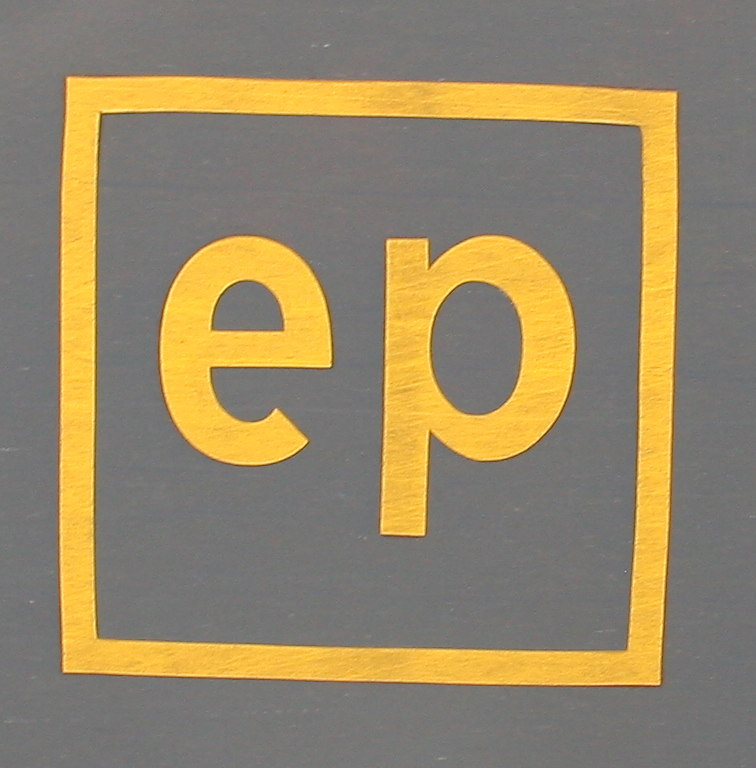
\includegraphics[width=2.5cm]{skryptkierownik-img/skryptkierownik-img028.jpg}
	& pojazd wyposażony w hamulec elektropneumatyczny\\
	\hline
	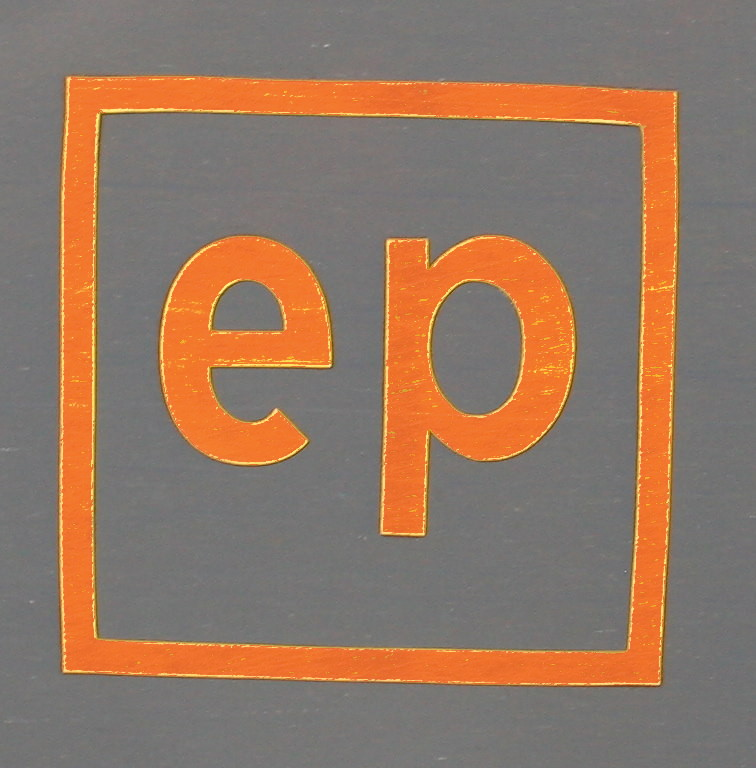
\includegraphics[width=2.5cm]{skryptkierownik-img/skryptkierownik-img029.jpg}
	& pojazd wyposażony w przewód przelotowy do sterowania hamulca elektropneumatycznego\\
	\hline
	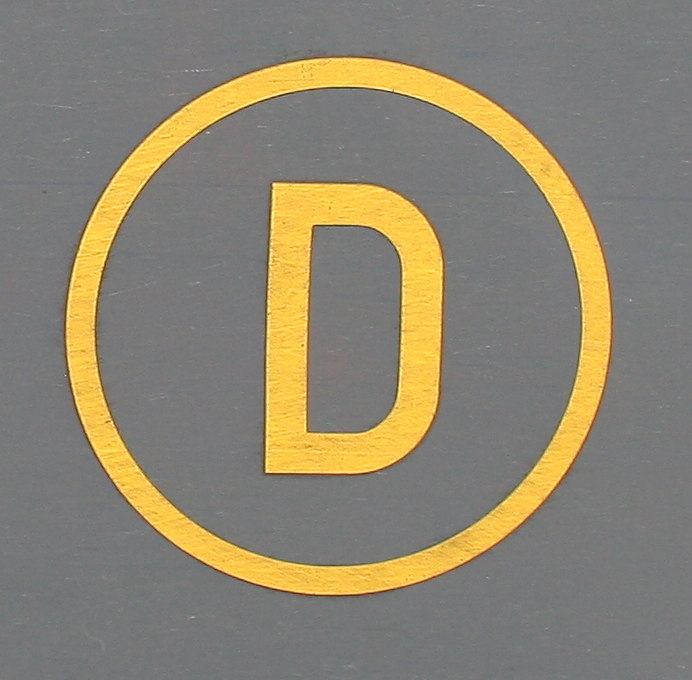
\includegraphics[width=2.5cm]{skryptkierownik-img/skryptkierownik-img030.jpg} & Hamulec tarczowy\\
	\hline
	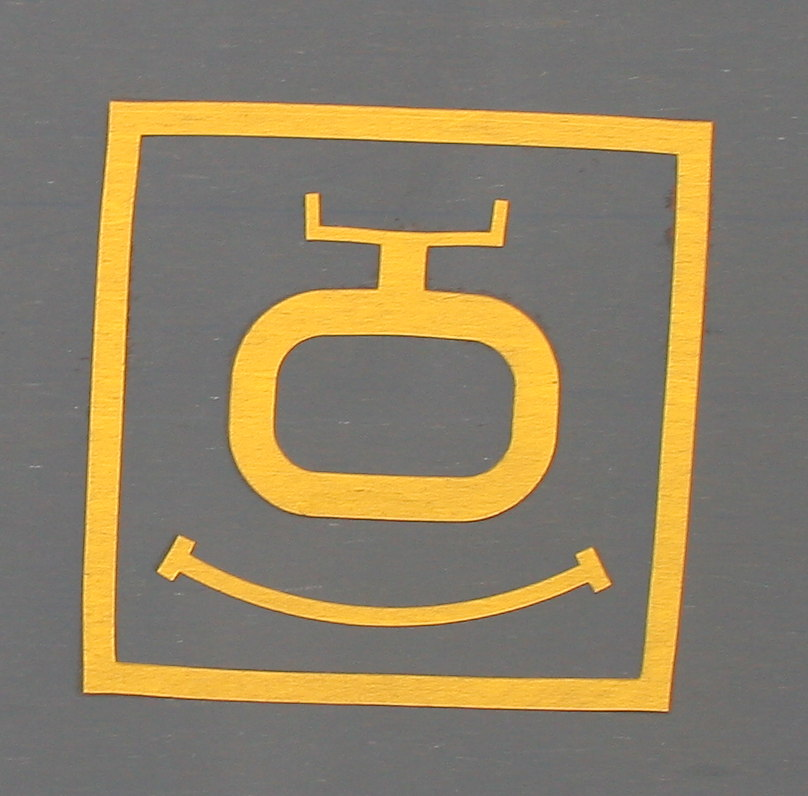
\includegraphics[width=2.5cm]{skryptkierownik-img/skryptkierownik-img031.jpg} & Mostkowanie hamulca bezpieczeństwa\\
	\hline
	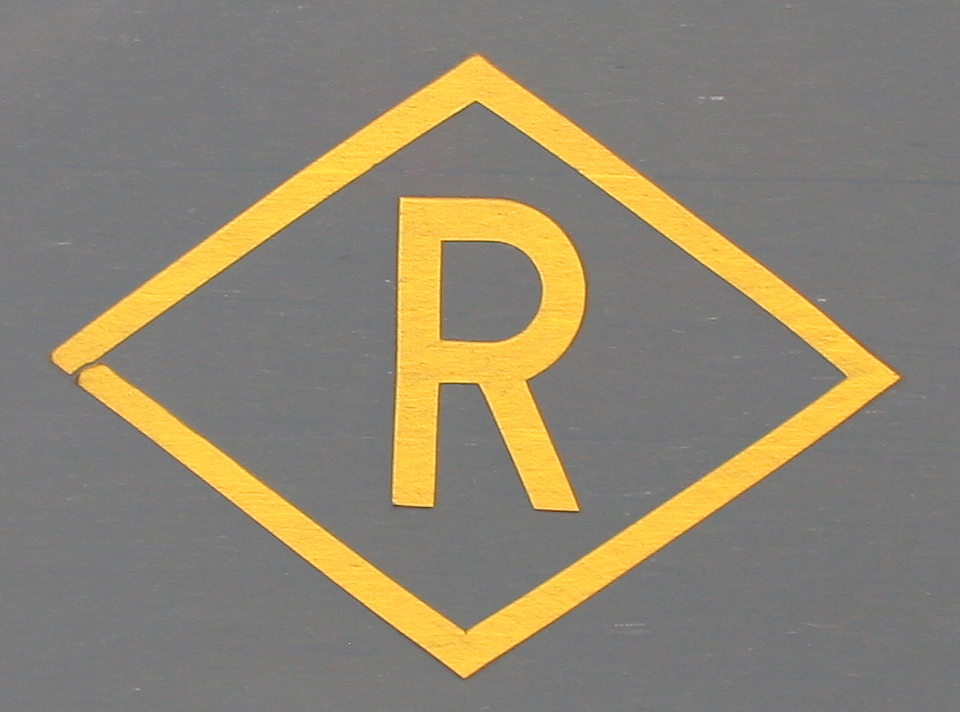
\includegraphics[width=2.5cm]{skryptkierownik-img/skryptkierownik-img032.jpg} & na nastawieniu R ("pospieszny") hamulec zapewnia procent masy hamującej wagonu próżnego od 150\% do 170\%\\
	\hline
\end{tabular}
\end{table*} 

\chapter{Obsługa urządzeń wagonowych}

Typowe urządzenia wagonowe to:

\begin{itemize}
	\item toaleta
	\item ogrzewanie i klimatyzacja
	\item oświetlenie
	\item drzwi
	\item hamulec bezpieczeństwa
	\item rampa/winda/podnośnik dla osób niepełnosprawnych
	\item światła końca pociągu
\end{itemize}

\begin{table*}
	\caption{Oznaczenia wyposażenia wagonowego}
	\label{tab:opisywagonowe}
	\begin{tabular}{|c|m{8cm}|}
		\hline
		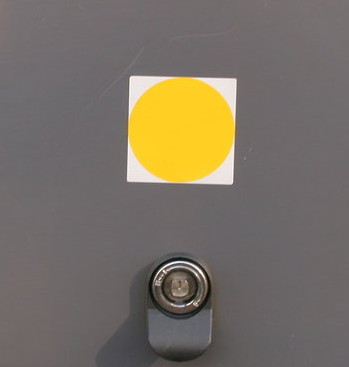
\includegraphics[width=2.5cm]{skryptkierownik-img/skryptkierownik-img035.jpg} & Złącze do wodowania\\
		\hline
	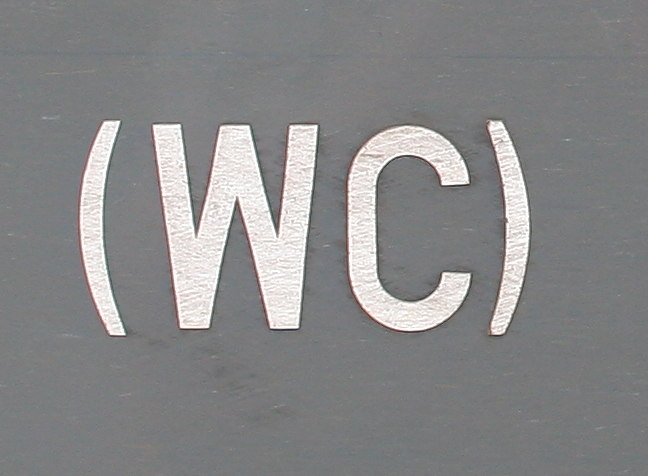
\includegraphics[width=2.5cm]{skryptkierownik-img/skryptkierownik-img036.jpg} & Wagon wyposażony w WC w układzie zamkniętym\\
	\hline
		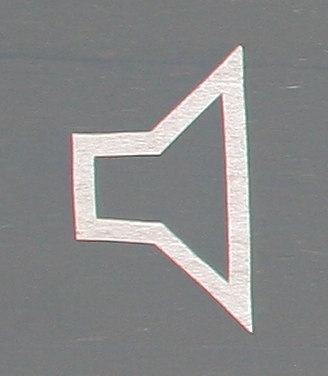
\includegraphics[width=2cm]{skryptkierownik-img/skryptkierownik-img037.jpg} & Wagony z instalacją głośnikową, bez możliwości dołączenia zewnętrznych urządzeń\\\hline
	\end{tabular}
\end{table*}
\pagebreak
\section{Toalety}
	\begin{figure}
\subfloat{	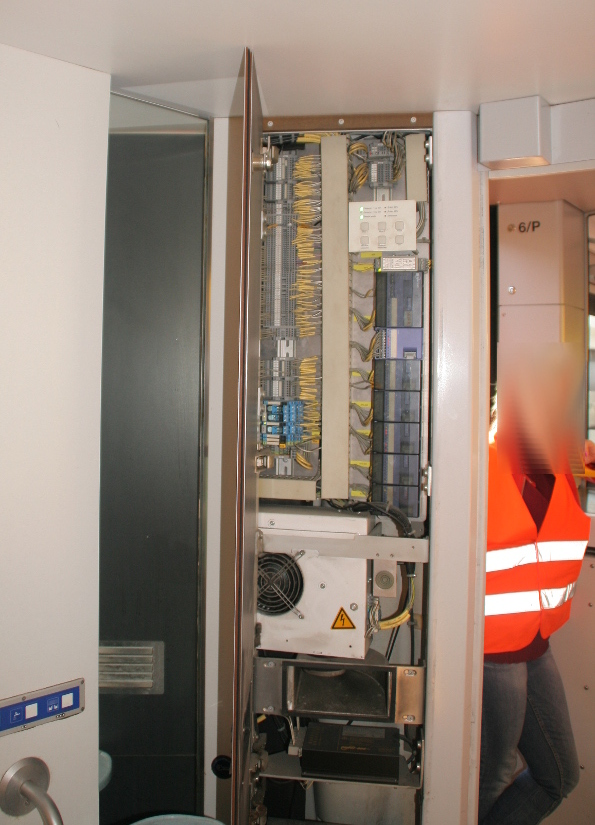
\includegraphics[width=6cm]{skryptkierownik-img/skryptkierownik-img038.jpg}}
\subfloat{	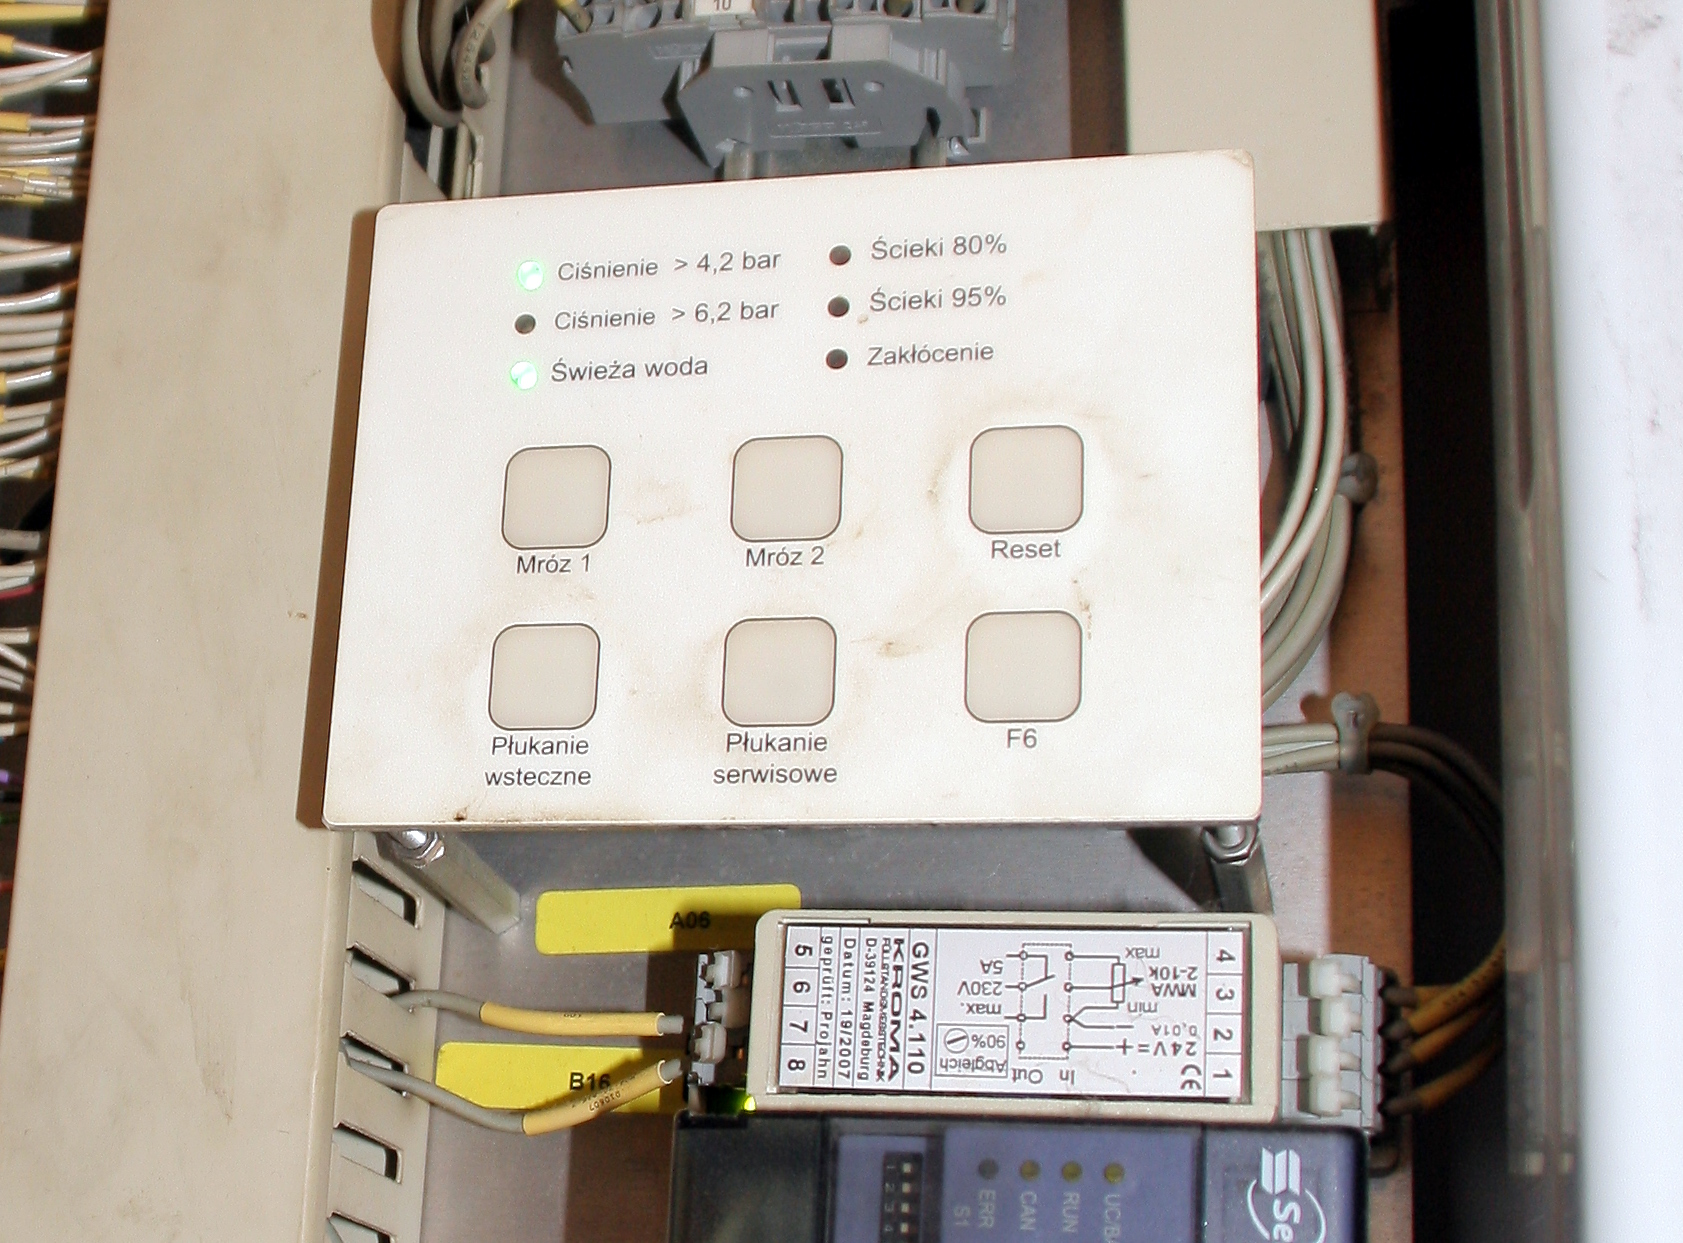
\includegraphics[width=6cm]{skryptkierownik-img/skryptkierownik-img039.jpg}}
	\caption{Dostęp do sterownika toalety EN75}
\end{figure}
	W pojazdach serii \textbf{EN75 Stadler Flirt} toaleta znajduje się w członie C. W toalecie, bezpośrednio przy wejściu, nad koszem na śmieci znajduje się sterownik WC. Pokrywa otwierana kluczem konduktorskim oraz kluczem patentowym z pojazdu przeznaczonym dla kierownika pociągu. Na sterowniku znajdują się opisane klawisze do wykonania miękkiego resetu, płukania serwisowego (twardy rewers), opróżniania mrozowego przewodów,etc.

W słupku bocznym na końcu wagonu w którym znajduje się toleta pod pokrywą opisaną symbolem CPX1 znajdują się bezpieczniki klimatyzacji, oświetlenia wagonu, oraz zasilania WC.

\begin{figure}
		\includegraphics[width=10cm]{skryptkierownik-img/skryptkierownik-img040.jpg}
		\caption{EN75 - Wnętrze szafki. Po prawej stronie widoczne bezpieczniki - w górnym rzędzie znajdują się bezpieczniki WC}
\end{figure}
\begin{figure}
\subfloat{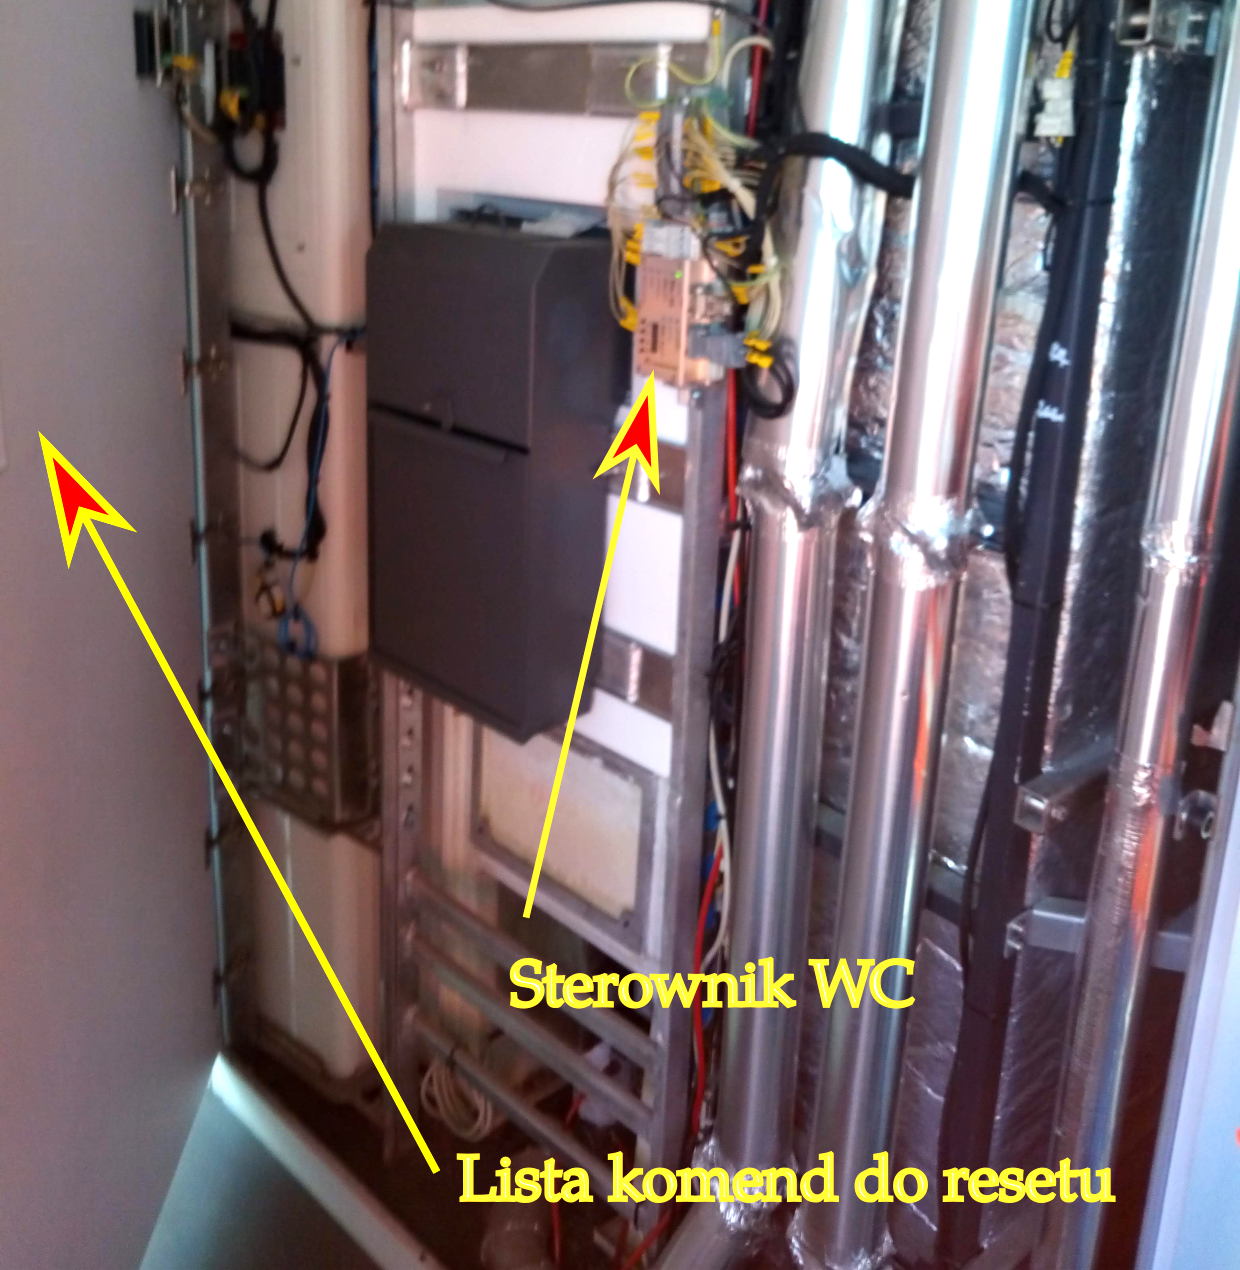
\includegraphics[width=5.5cm]{skryptkierownik-img/skryptkierownik-img055.png}}
\subfloat{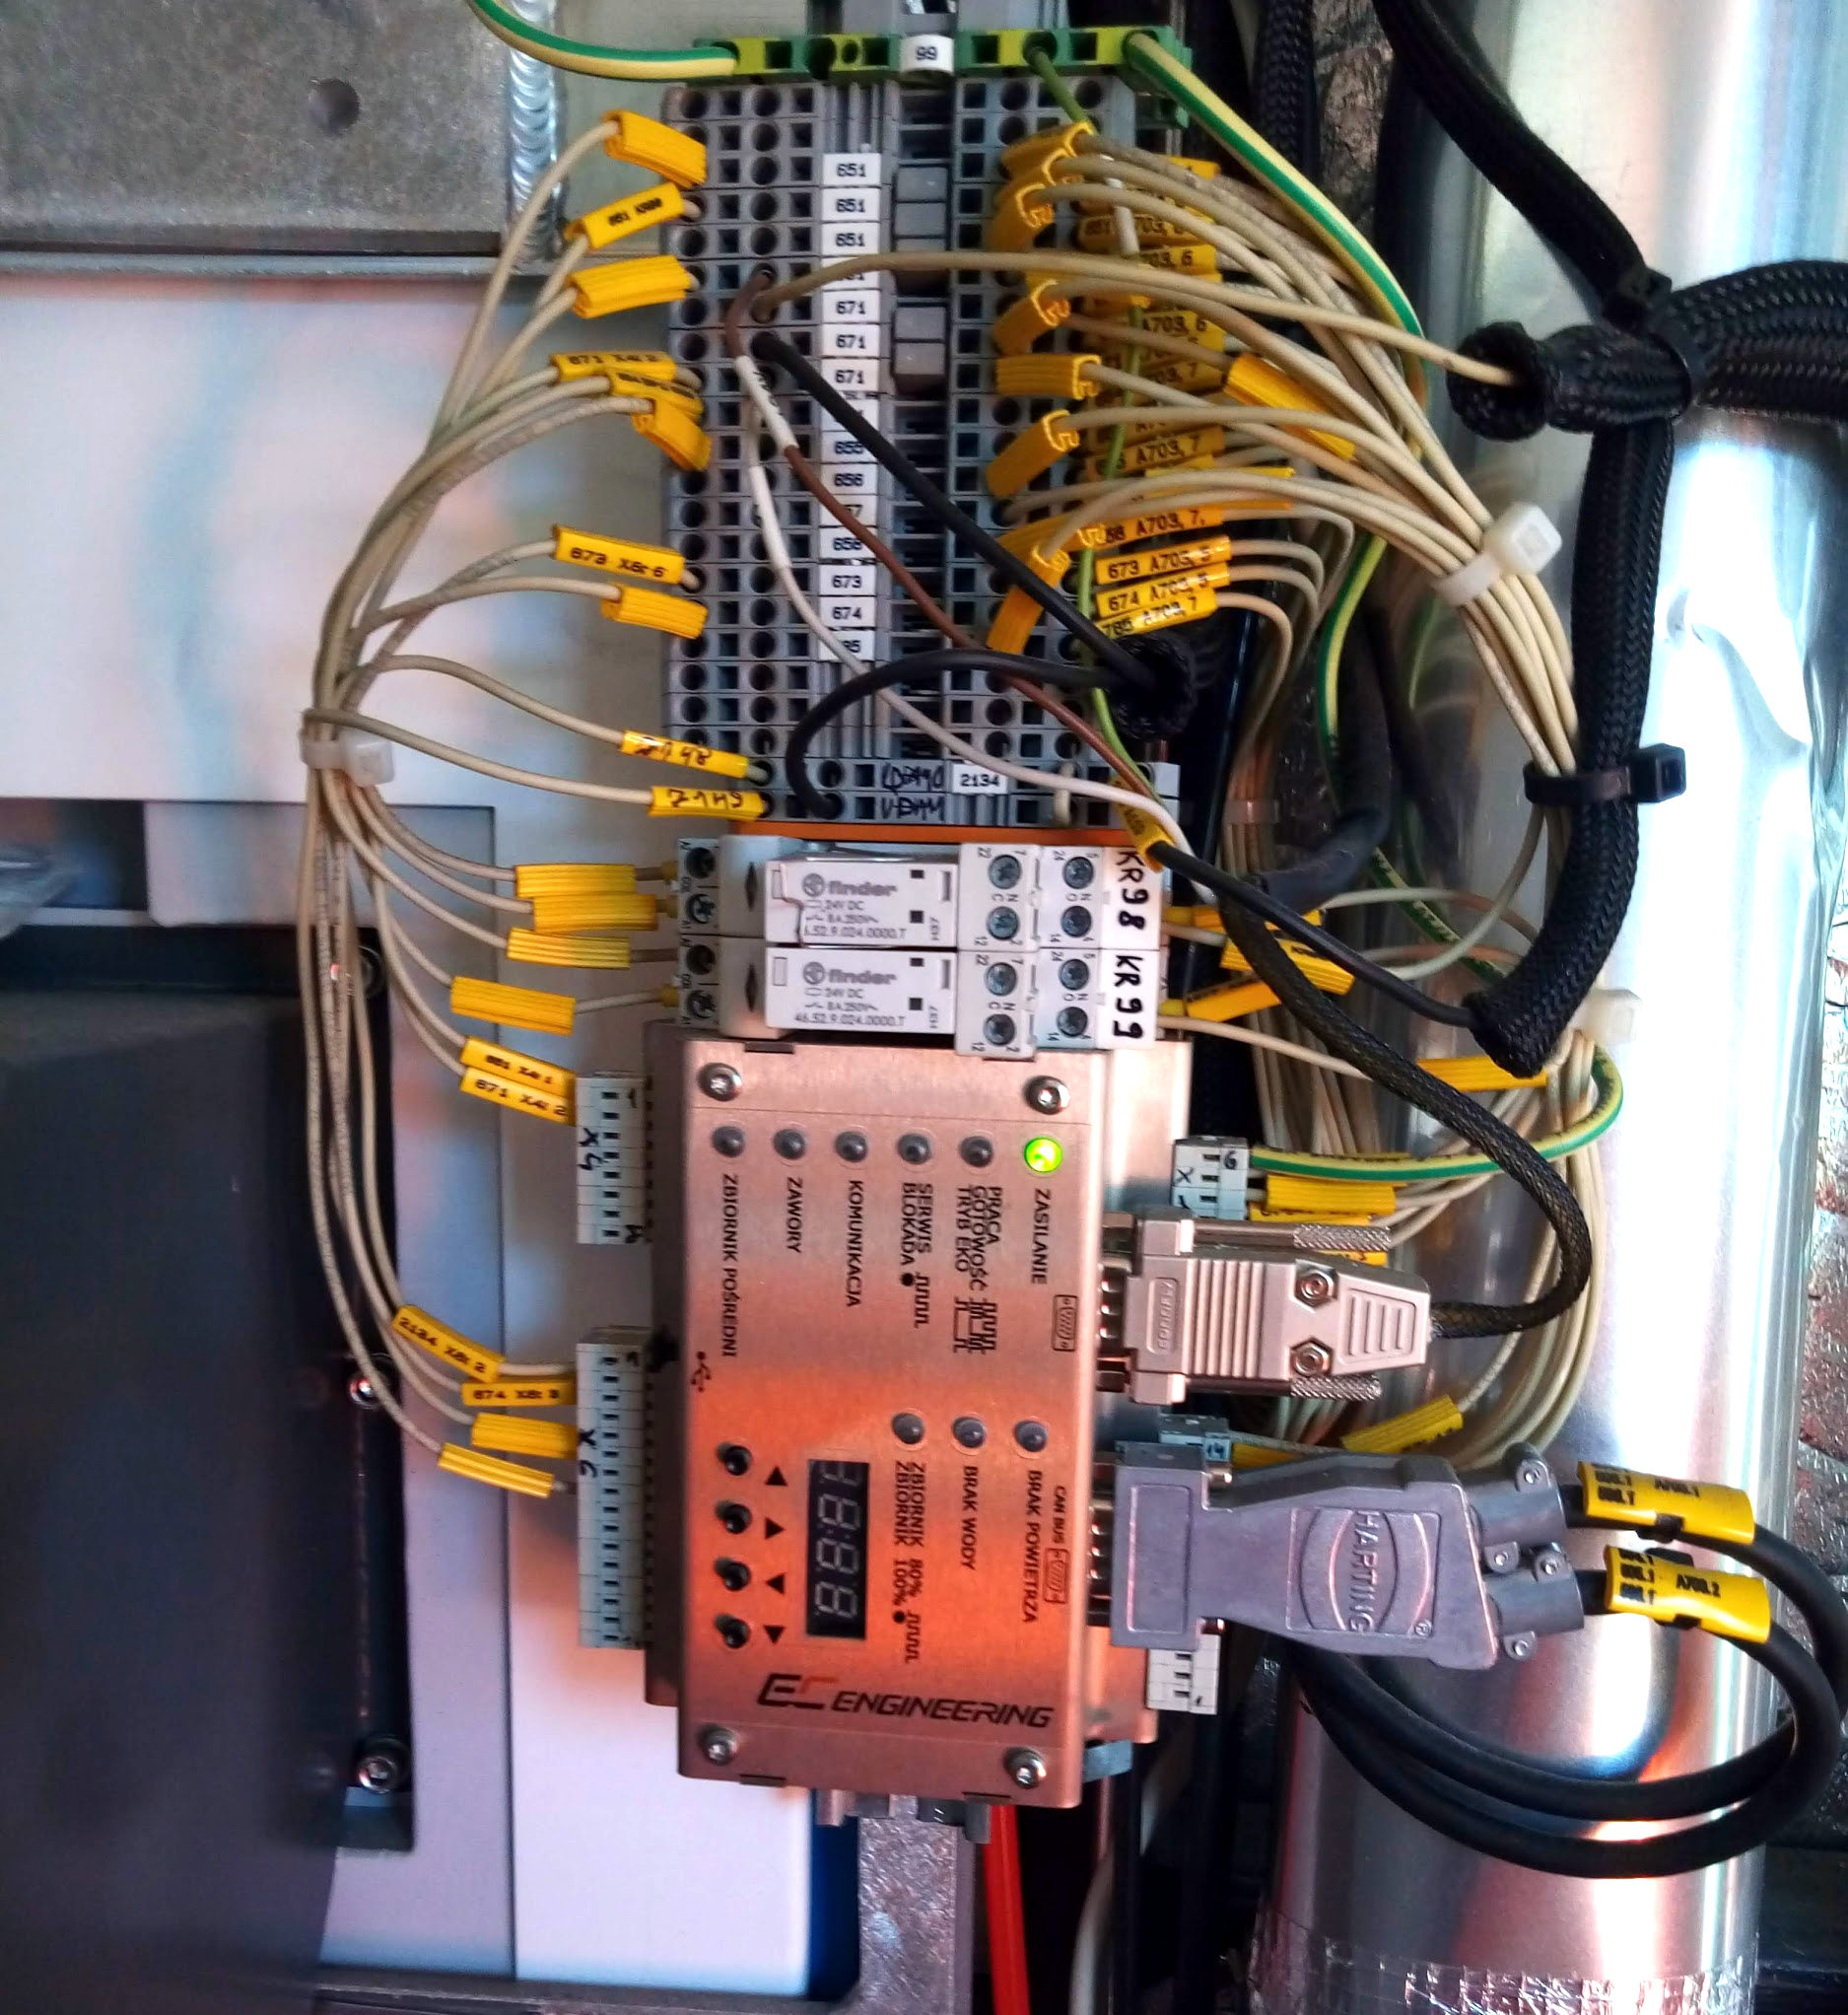
\includegraphics[width=5.5cm]{skryptkierownik-img/skryptkierownik-img056.jpg}}
	\caption{Elf 2 - Z lewej lokalizacja sterownika w luku rewizyjnym, z prawej sterownik}	
\end{figure}
W pojazdach serii \textbf{Elf 2} toaleta znajduje się w członie A (w 34WEa), lub C (w pozostałych pojazdach trzy i czteroczłonowych) Aby wykonać uzdatnienie WC należy otworzyć kluczem konduktorskim i kluczem patentowym zamki na zewnątrz WC od strony przejścia. W środkowej części otwartej przestrzeni znajduje się sterownik WC z czterema przyciskami. Wykonanie odpowiedniej operacji polega na \textbf{równoczesnym }wciśnięciu odpowiednich przycisków. Informacja o kombinacji przycisków znajduje się na wewnętrznej części pokrywy. Dla wykonania “twardego rewersu” należy dodatkowo potwierdzić operację (wskazanym przyciskiem).
\begin{figure}
	
\includegraphics[width=10cm]{skryptkierownik-img/wc-elf2.png}
	\caption{Kombinacje przycisków na sterowniku WC w pojazdach Elf2}
\end{figure}
\begin{marginfigure}
	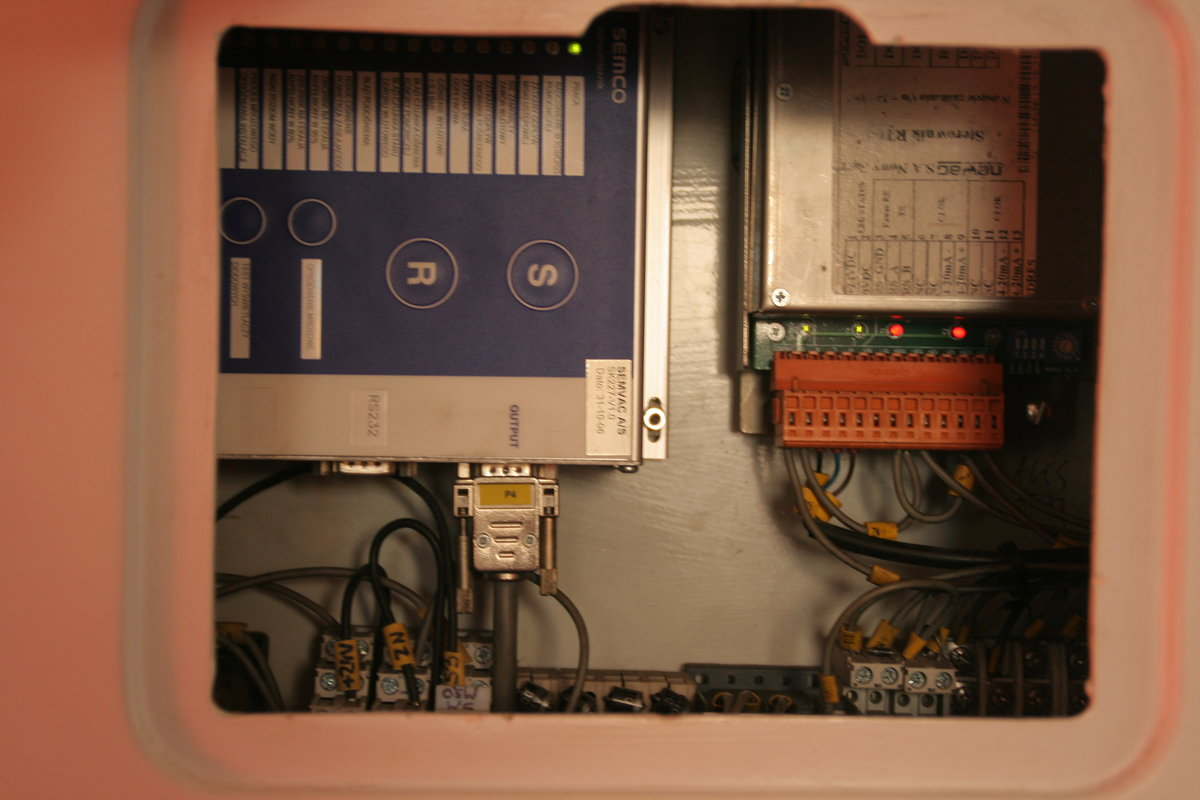
\includegraphics[width=5.5cm]{skryptkierownik-img/skryptkierownik-img057.jpg}
	\caption{Sterownik WC toalet w pojazdach produkcji Newagu}
\end{marginfigure}
W pojazdach produkcji firmy Newag (EN57AKŚ, EN71AKŚ, 35WE, 36WEa) sterownik toalety znajduje się na zewnętrznej stronie ściany toalety. Pod pokrywą zamykaną kluczem konduktorskim można dokonać płukania (rewersu) „miękkiego” lub serwisowego. Dodatkowo, powyżej sterownika, znajduje się przełącznik wyłączenia zasilania toalety, przy pomocy którego możemy na przykład znieść blokadę drzwi.

\begin{figure}
	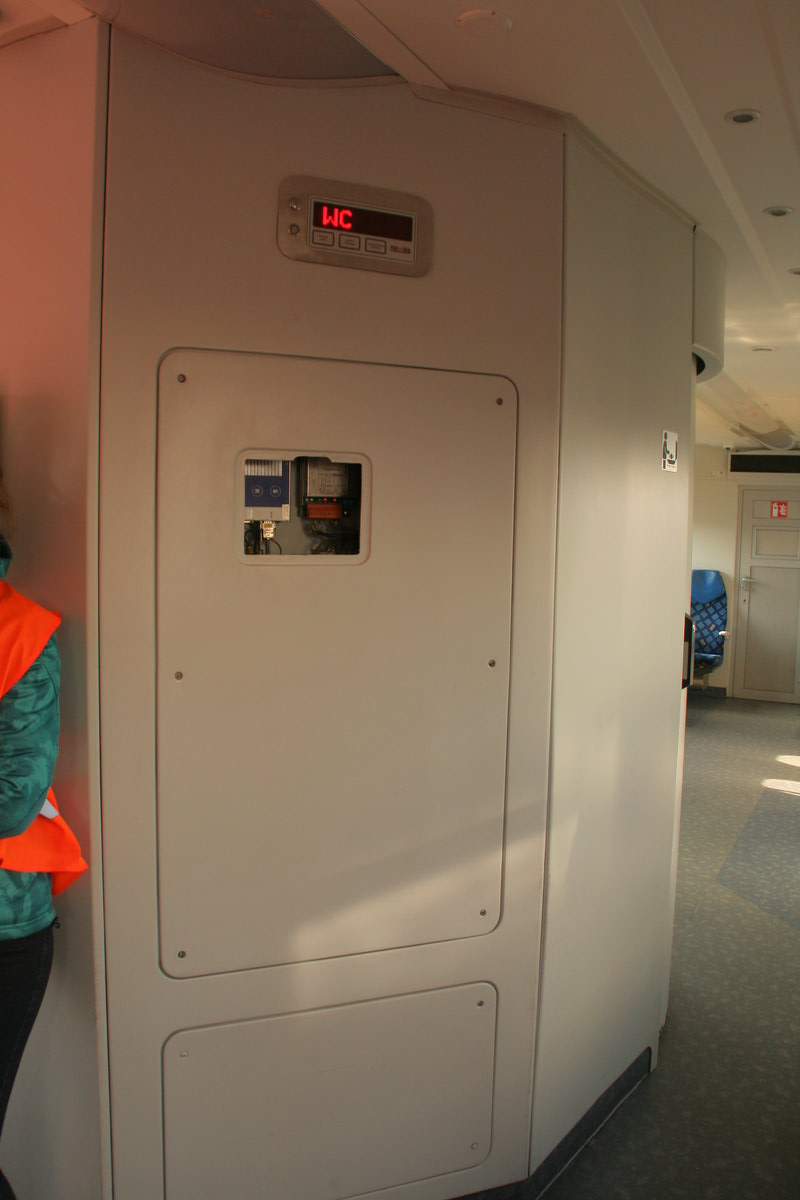
\includegraphics[width=5.5cm]{skryptkierownik-img/skryptkierownik-img058.jpg}
	\caption{Lokalizacja sterownika toalety w pojazdach firmy Newag}
\end{figure}

W pojazdach typu EN76 i 27WEb sterownik toalety znajduje się wewnątrz WC, za lustrem otwieranym przy pomocy klucza konduktorskiego. Sposób sterowania jest analogiczny do tego z pojazdów typu EN57AKŚ (przyciski dla płukania wstecznego i płukania serwisowego).

\section{Podnośnik dla osób niepełnosprawnych}
W pojazdach EN75 podnośnik znajduje się w członie C, obok toalety. Aby użyć podnośnika dla osób niepełnosprawnych, należy w pierwszej kolejności otworzyć kluczem kierownika pociągu zamek znajdujący się na obudowie zewnętrznej. Otworzyć drzwi wagonu, następnie pociągnąc za klamkę (pokrywę), i ustawić podnośnik równolegle do drzwi wejściowych – w tym czasie zamknie się stopień wejściowy i uruchomi sygnał ostrzegający.
Następnie wypchnąć płytę podnośnika poza pojazd (można wspomagać się dźwignią po prawej stronie), aż do pozycji leżącej. W kolejnym kroku otworzyć pokrywy/ograniczniki. Sterowanie podnośnikiem z przenośnego pilota czarnymi
klawiszami. Po podniesieniu rampy podnośnika z peronu spowrotem do wysokości wagonu, należy „dociągnąć” rampę przy pomocy żółtego przycisku na górnej części pilota.

Aby obsłużyć podnosnik awaryjnie należy wyłączyć zasilanie podnośnika bezpiecznikiem, następnie przekręcić śrubę pompy hydraulicznej i pociągnąć za czerwoną rączkę aby opuszczać rampę podnośnika. Następnie należy dokręcić śrubę i umieścić
we wskazanym miejscu w lewarku pompy drążek. Przy pomocy lewarka można podnieść rampę i wciągnąć ją do wagonu. Składanie rampy w odwrotnej kolejności do rozkładania.
	\begin{marginfigure}
	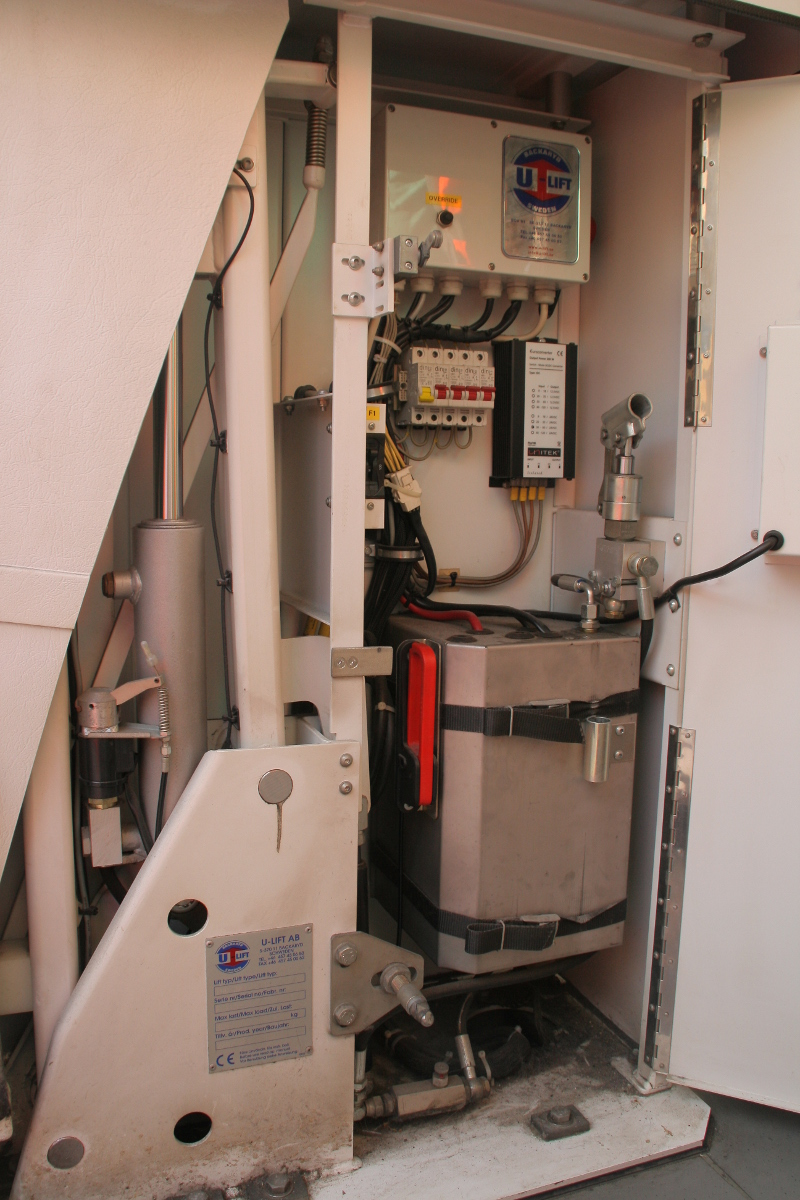
\includegraphics[width=5cm]{skryptkierownik-img/skryptkierownik-img041.jpg}
	\caption{Awaryjne (ręczne) sterowanie podnośnikiem}
\end{marginfigure}

W pojazdach Elf 2 podnośnik znajduje się obok toalety. Należy odblokować zamek drzwi i uchylić je, odblokować zamek
podnośnika przez pociągnięcie uchwytu do siebie. Następnie pociągnąć za uchwyt obracając podnośnik aż znajdzie się na
zewnątrz pojazdu. Po obrocie podnośnika o 180° zaskoczy zatrzask blokady jego osi obrotu blokując tym samym ruch
obrotowy.

Kolejne czynności:

\begin{itemize}
	\item opuścić platformę do poziomu.
	\item odciągnąć zatrzask i jednocześnie
	\item rozłożyć rozkładaną platformę środkową do poziomu obracając ją o
	\item 180°.
	\item odciągnąć zatrzask i jednocześnie otworzyć najazd zewnętrzny przez obrót o 90° (pozycja ta zostaje ustalona zatrzaskiem);
	\item otworzyć poręcz przez obrót o 90° (do pionu) do momentu  zatrząśnięcia rygla;
	\item odciągnąć zatrzask i jednocześnie otworzyć najazd wewnętrzny przez obrót o 90° (pozycja ta zostaje ustalona zatrzaskiem);
	\item Załączyć układ elektryczny podnośnika pokładowego przez obrót wyłącznika głównego w pole „I”.
\end{itemize}
\begin{marginfigure}
	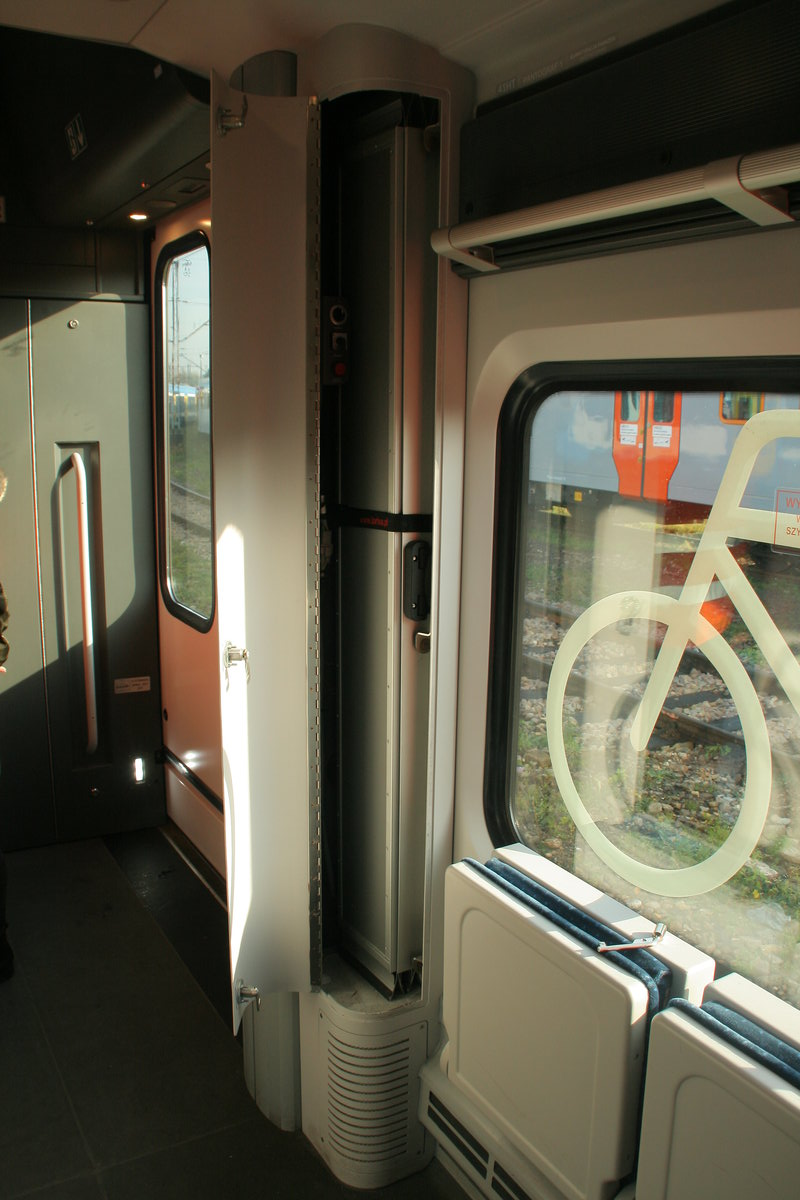
\includegraphics[width=5cm]{skryptkierownik-img/skryptkierownik-img053.jpg}
	\caption{Lokalizacja skrytki na rampę przenośną}
\end{marginfigure}
Sterowanie platformą wykonać można zarówno z poziomu pokładu jak i peronu.

Aby przygotować podnośnik do dalszej jazdy należy wykonać następujące czynności:

\begin{itemize}
	\item wyłączyć układ elektryczny podnośnika przez obrót wyłącznika głównego w położenie „0”;
	\item złożyć najazd wewnętrzny i zewnętrzny oraz poręcz;
	\item złożyć składaną platformę środkową;
	\item zamknąć platformę podnosząc ją do pozycji pionowej;
	\item złożyć podnośnik do pozycji „do transportu”, upewnić się, że zadziałał zatrzask blokujący podnośnik;
	\item zamknąć drzwi obudowy.
\end{itemize}
W przypadku awarii pompy elektrycznej lub sterowania podnośnika można opuścić lub podnieść go w następujący sposób:
- ruch podnośnika „do góry” realizowany jest poprzez pompę ręczną (pokrętło zaworu awaryjnego wykręcone w lewo)
- ruch podnośnika „na dół” uzyskuje się przez przekręcenie (w prawo) pokrętła zaworu awaryjnego opuszczania

\begin{marginfigure}
	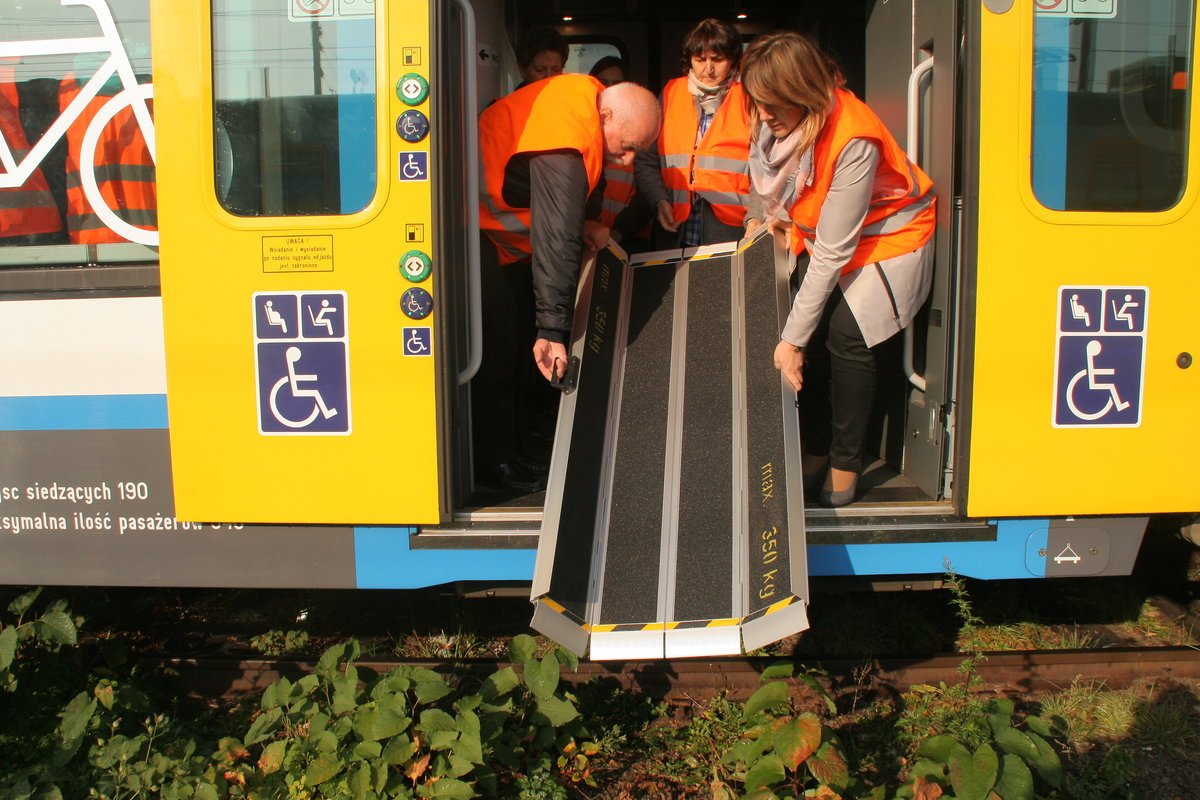
\includegraphics[width=5cm]{skryptkierownik-img/skryptkierownik-img054.jpg}
	\caption{Rozkładanie rampy}
\end{marginfigure}
Dodatkowo istnieje możliwość skorzystania z przenośnej rampy którą można rozłożyć na wysokich peronach, aby umożliwić wjazd wózka o własnych siłach. Rampa znajduje się w słupku bocznym drzwi na przeciwko toalety. 

W pojazdach typu AKŚ (EN57, EN71), w celu rozłożenia rampy podjazdowej dla osób niepełnosprawnych należy odkręcić kluczem konduktorskim zamek rampy, obrócić ją wokół osi do drzwi, a następnie odblokować zapadkę (pałąk zabezpieczający). Tak przygotowaną rampę wystarczy od strony peronu pociągnąć za uchwyty do rozłożenia. Składanie w odwrotnej kolejności. Uwaga! W stanowisku rampy znajduje się czujnik jej poprawnego zamknięcia który może uniemożliwić uruchomienie napędu.

\begin{figure}
\subfloat{	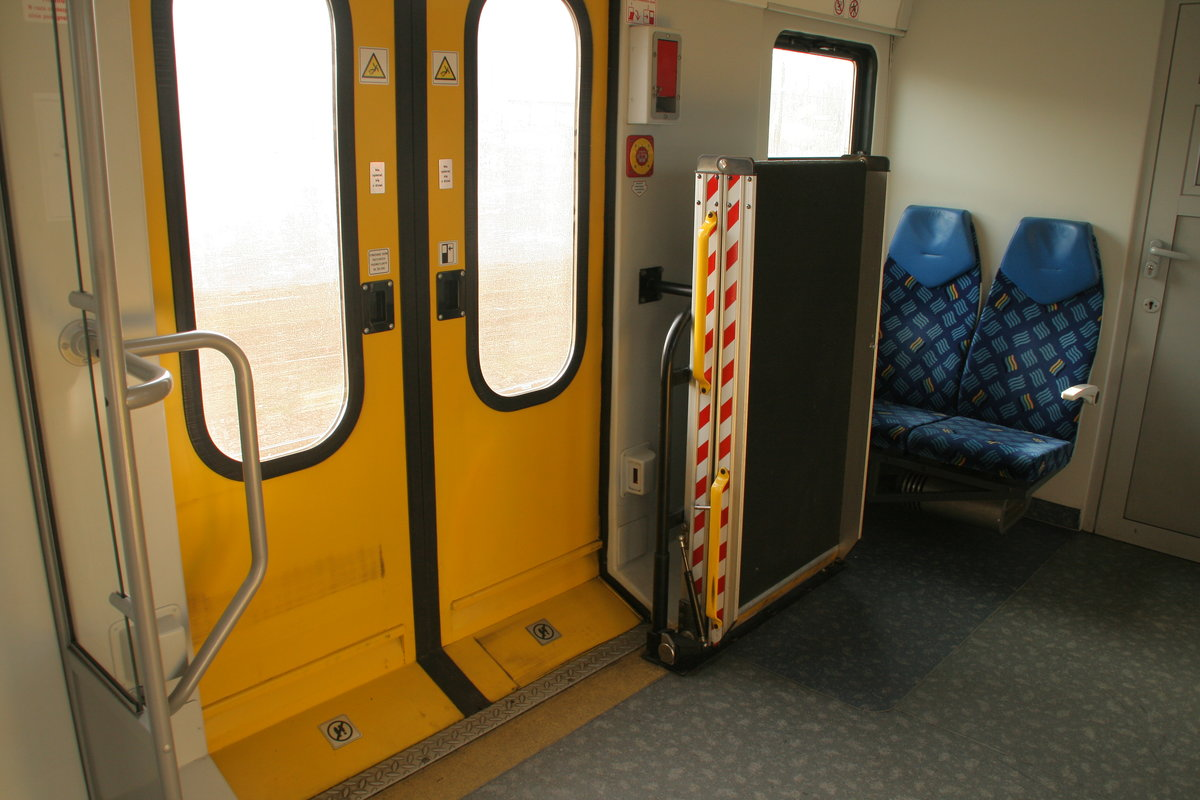
\includegraphics[width=6cm]{skryptkierownik-img/skryptkierownik-img060.jpg}}
	\subfloat{ 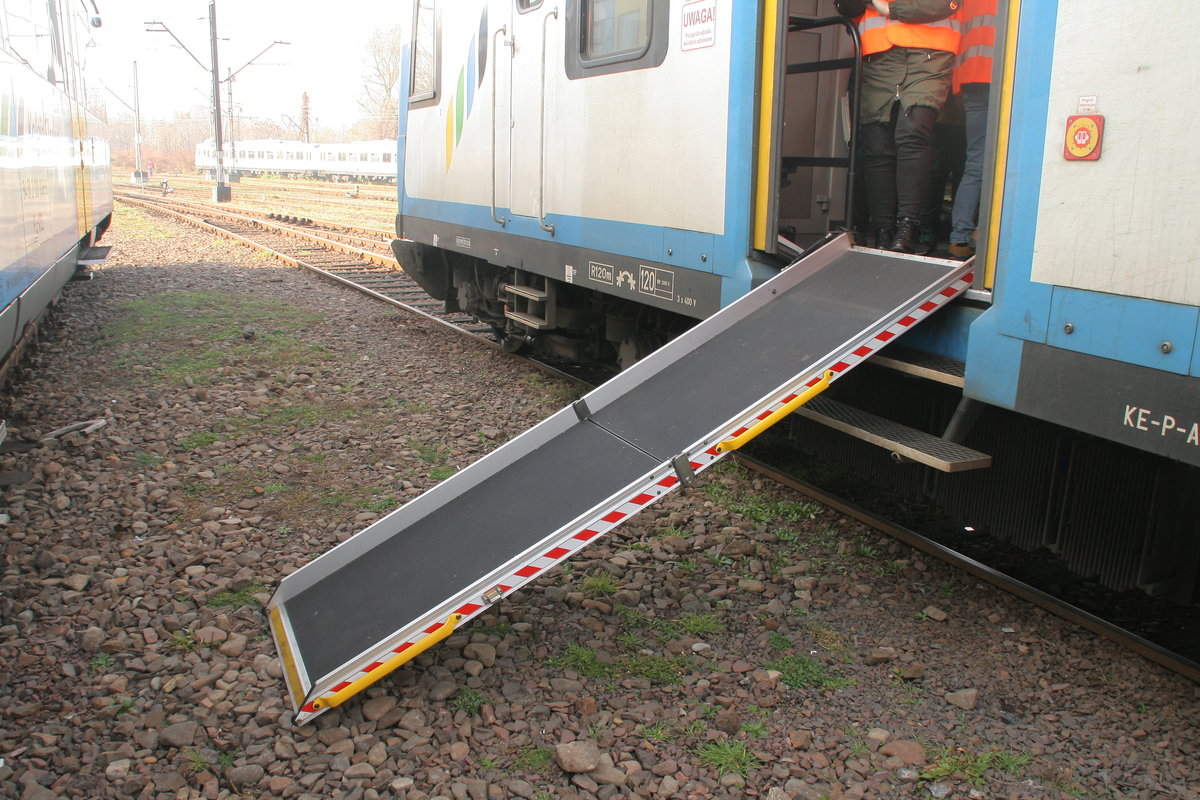
\includegraphics[width=6cm]{skryptkierownik-img/skryptkierownik-img063.jpg}}
	\caption{Ogólny widok drzwi i rampy, z prawej rampa rozłożona poza pojazd}
\end{figure}


\begin{figure}
	\subfloat{	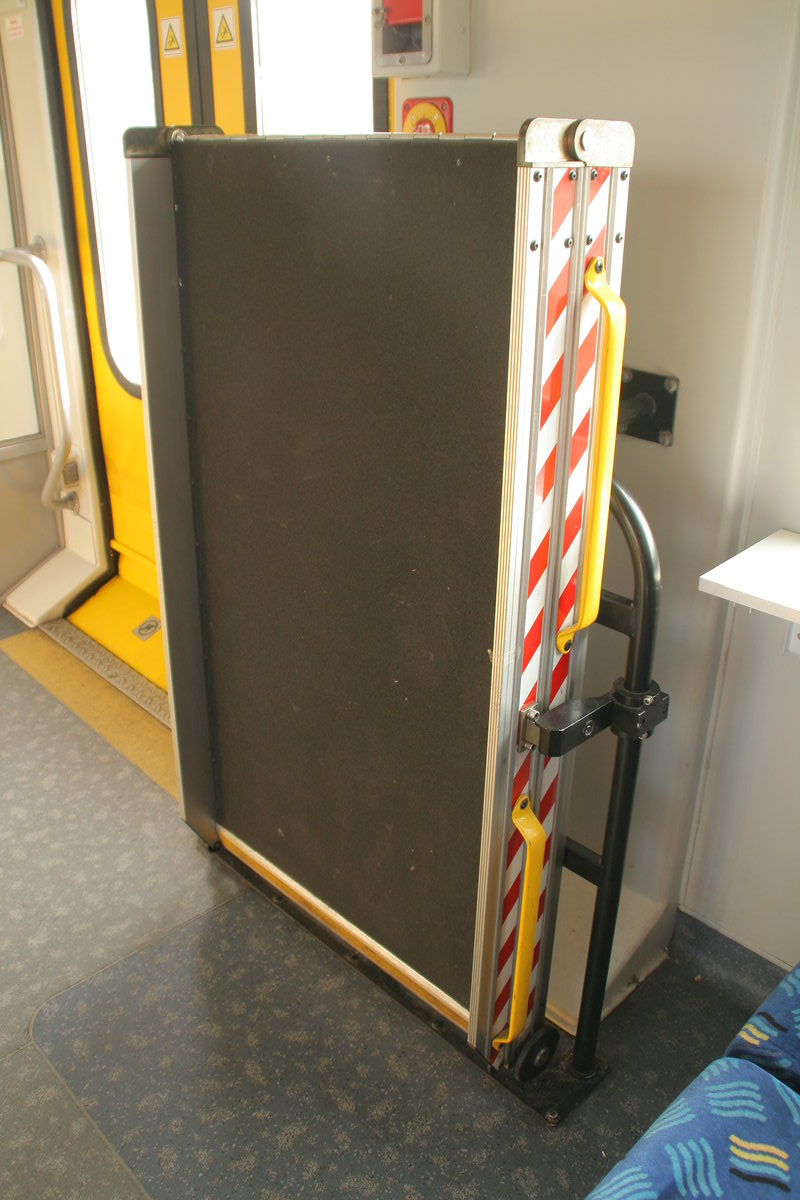
\includegraphics[width=6cm]{skryptkierownik-img/skryptkierownik-img061.jpg}}
	\subfloat{	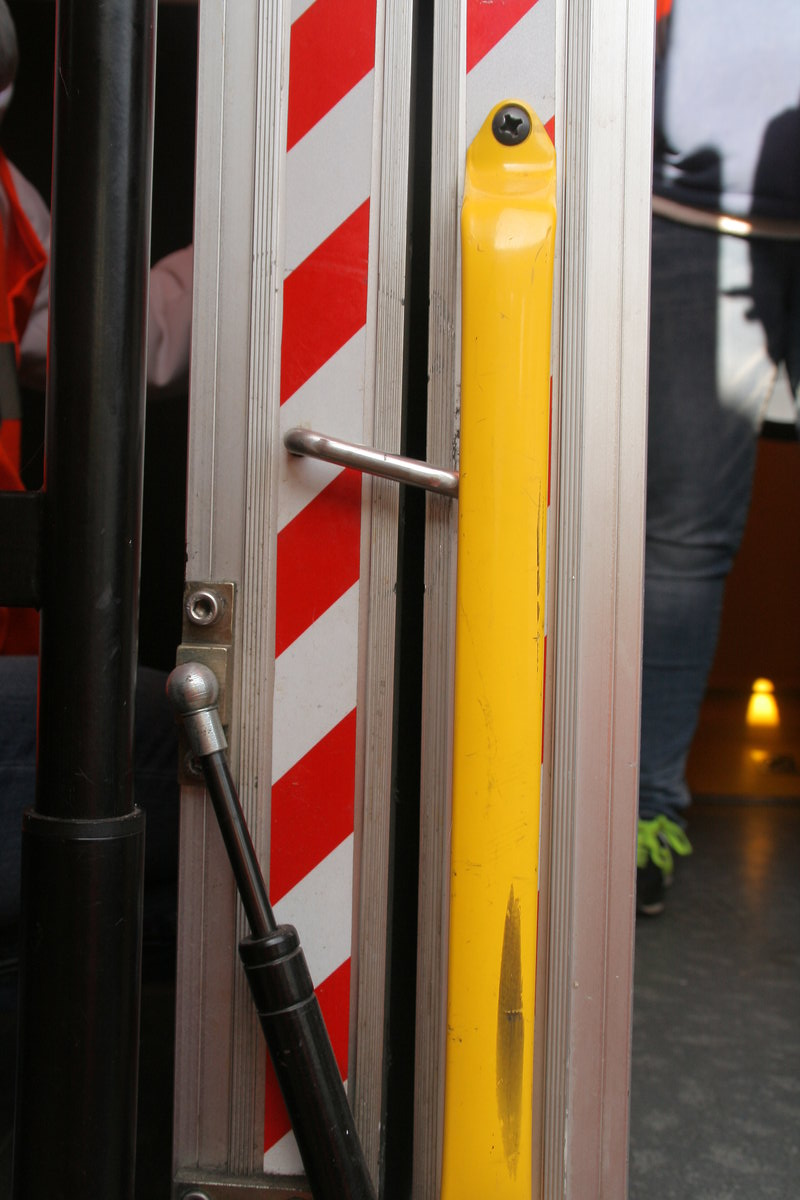
\includegraphics[width=6cm]{skryptkierownik-img/skryptkierownik-img062.jpg}}
	\caption{Zamek zabezpieczający rampę, Pałąk zabezpieczenia}
\end{figure}

\section{Drzwi}
W pojazdach EN75, EN76, 27WEb w dolnej części skrzydła drzwi znajduje się zamek na klucz konduktorski który pozwala na wyłączenie/odcięcie sterowania drzwi. W pojazdach 21WEa, 22WEd, 34WEa w lewej ściance znajduje się zamykana na klucz konduktorski oraz zamek (klucz kierownika pociągu) szafa sterownika drzwi.
	\begin{marginfigure}
		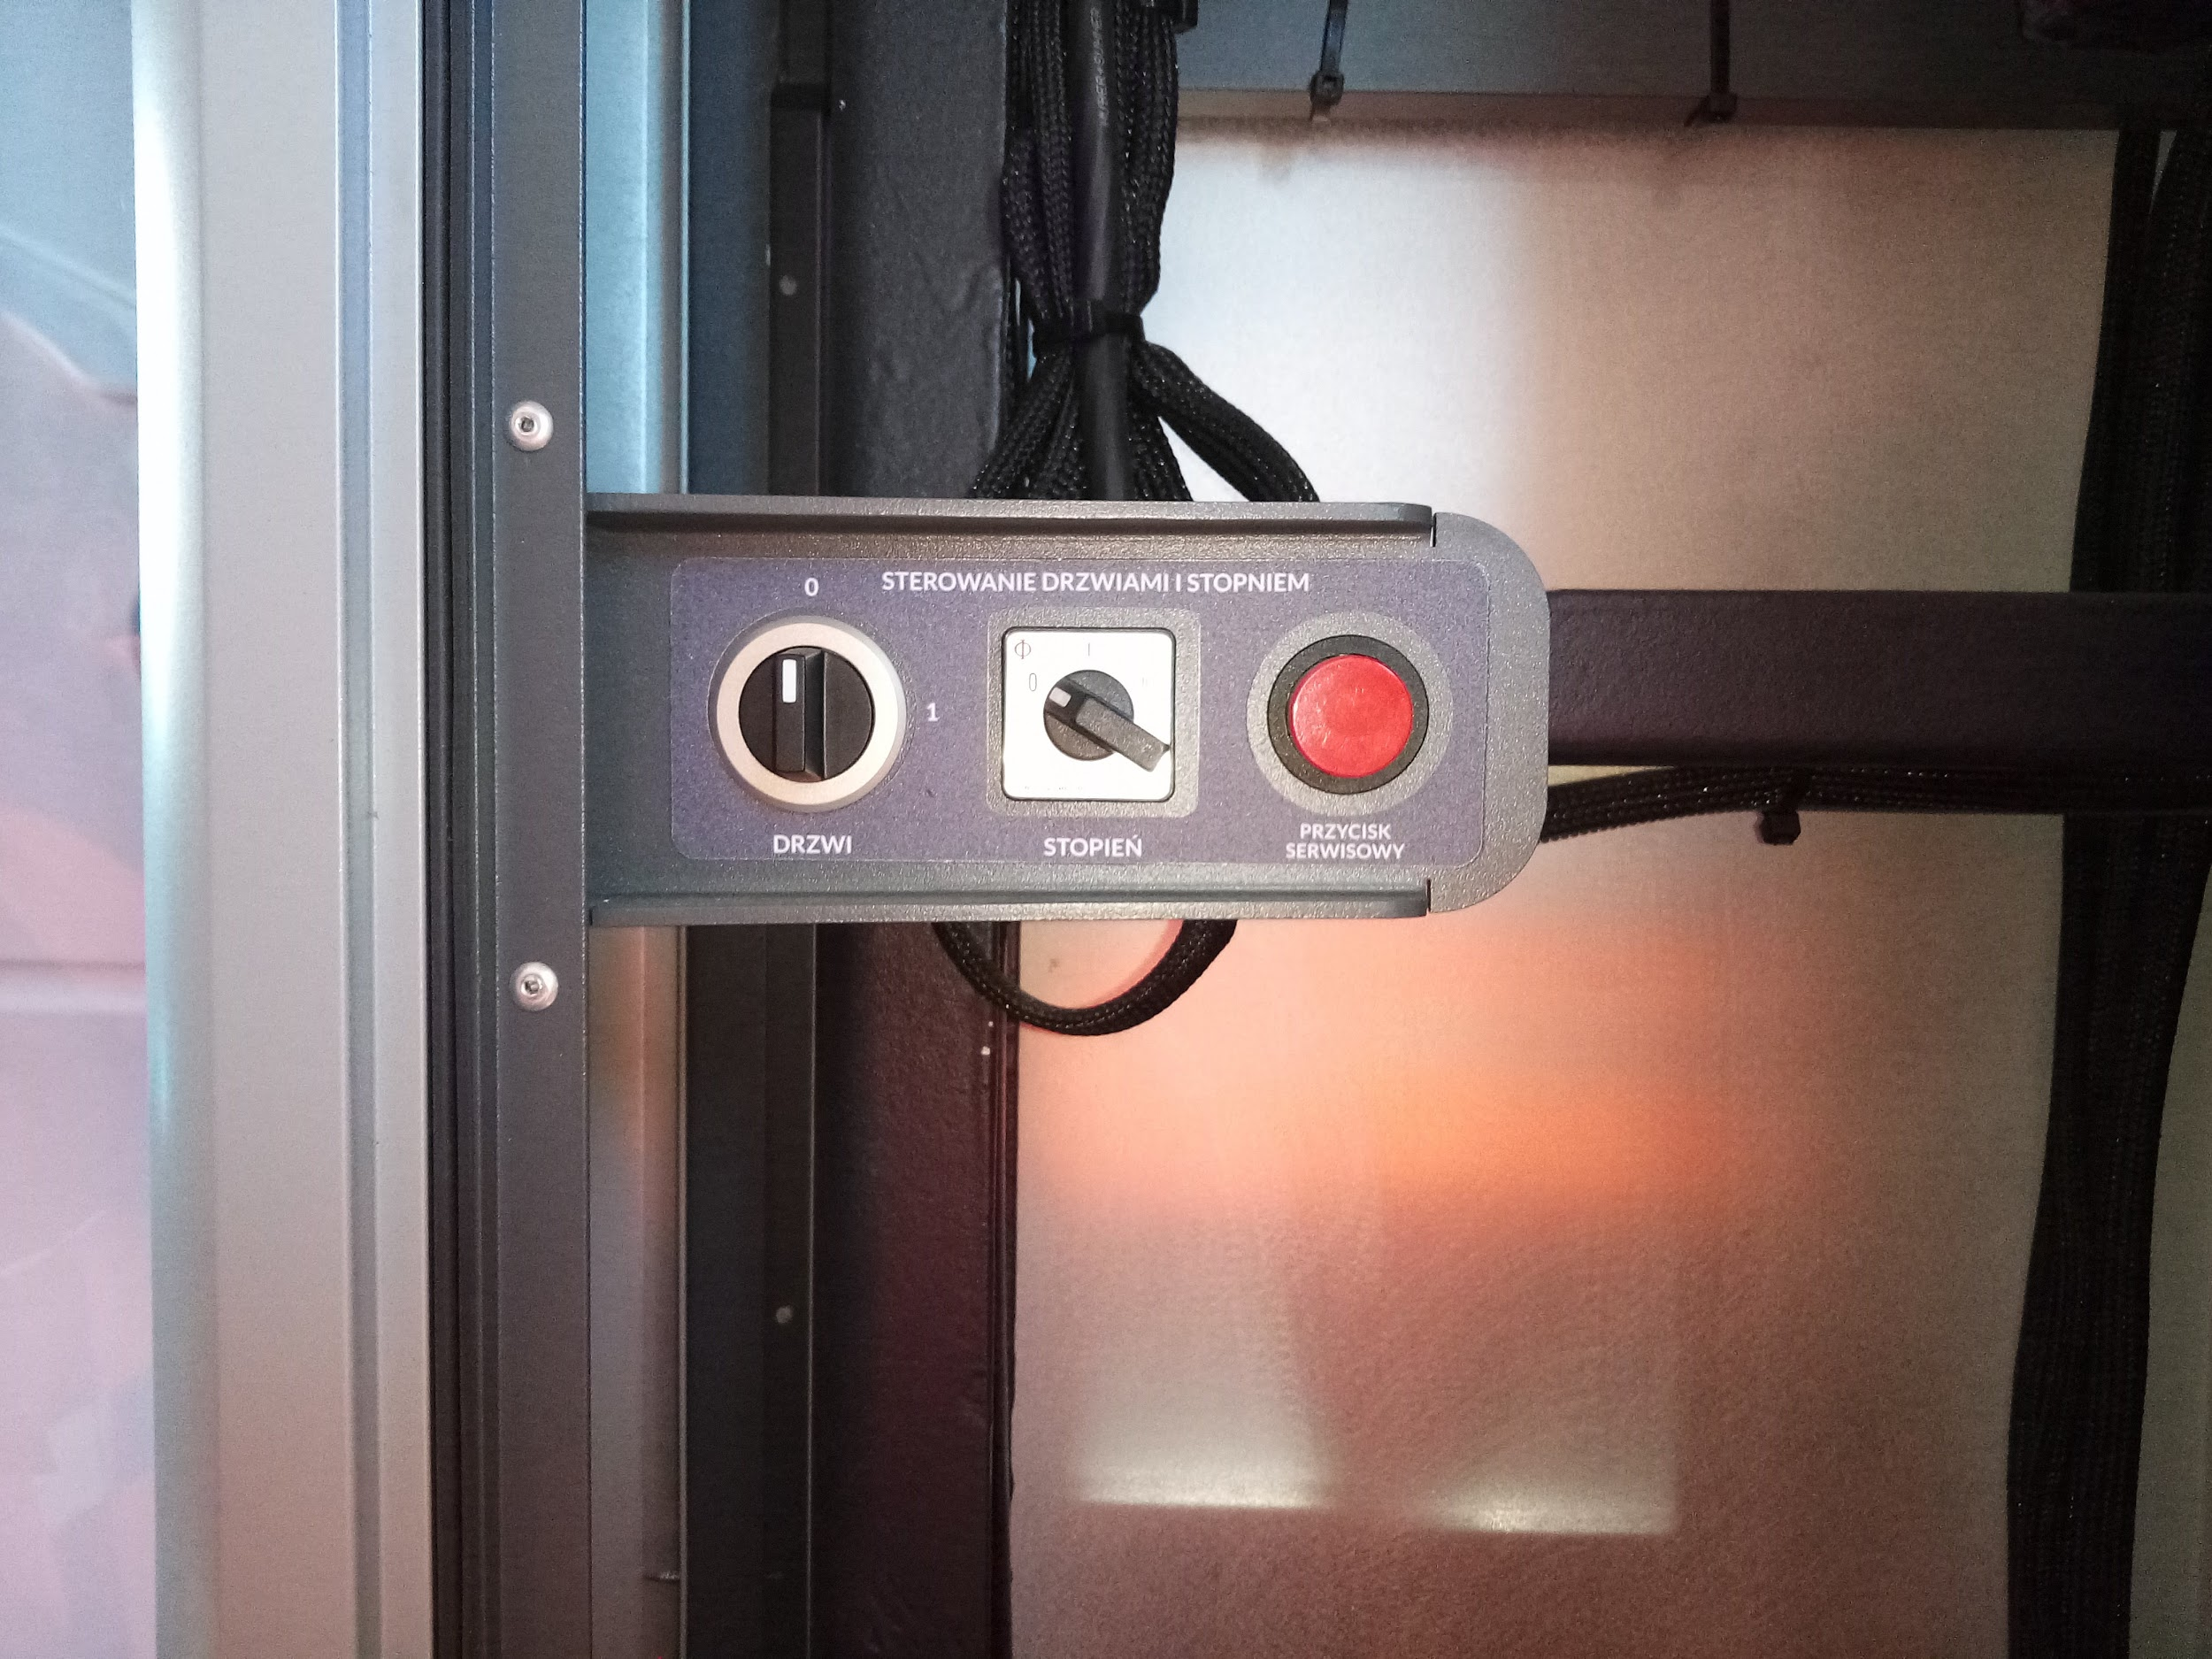
\includegraphics[width=6cm]{skryptkierownik-img/skryptkierownik-img048.jpg}
		\caption{Elf2 - Przełączniki sterownika drzwi}
	\end{marginfigure}

Pierwszy od strony lewej przełącznik służy do resetu (pozycja podstawowa opisana jako “0”, chwilowe przełączenie na pozycję “1” spowoduje zresetowanie sterownika), środkowy przełącznik stopnia (w pozycji “0” - podstawowa, “1” - ręczne chowanie stopnia, “2” - stopień wyłączony). Prawy, czerwony przycisk jest przyciskiem serwisowym, który spowoduje natychmiastowe otwarcie drzwi, np. w przypadku awarii??.

Po zatrzymaniu pojazdu V=0km/h, istnieje możliwość otwarcia pierwszej pary drzwi wraz ze stopniem, aby otworzyć drzwi należy posłużyć się kluczem kierownika pociągu przekręcając w prawo przełącznik widoczny na prawym zdjęciu – po przekręceniu łącznik powraca w pierwszą pozycję). Zamknięcie wykonujemy powtarzając operację.
	\begin{figure}
		\subfloat{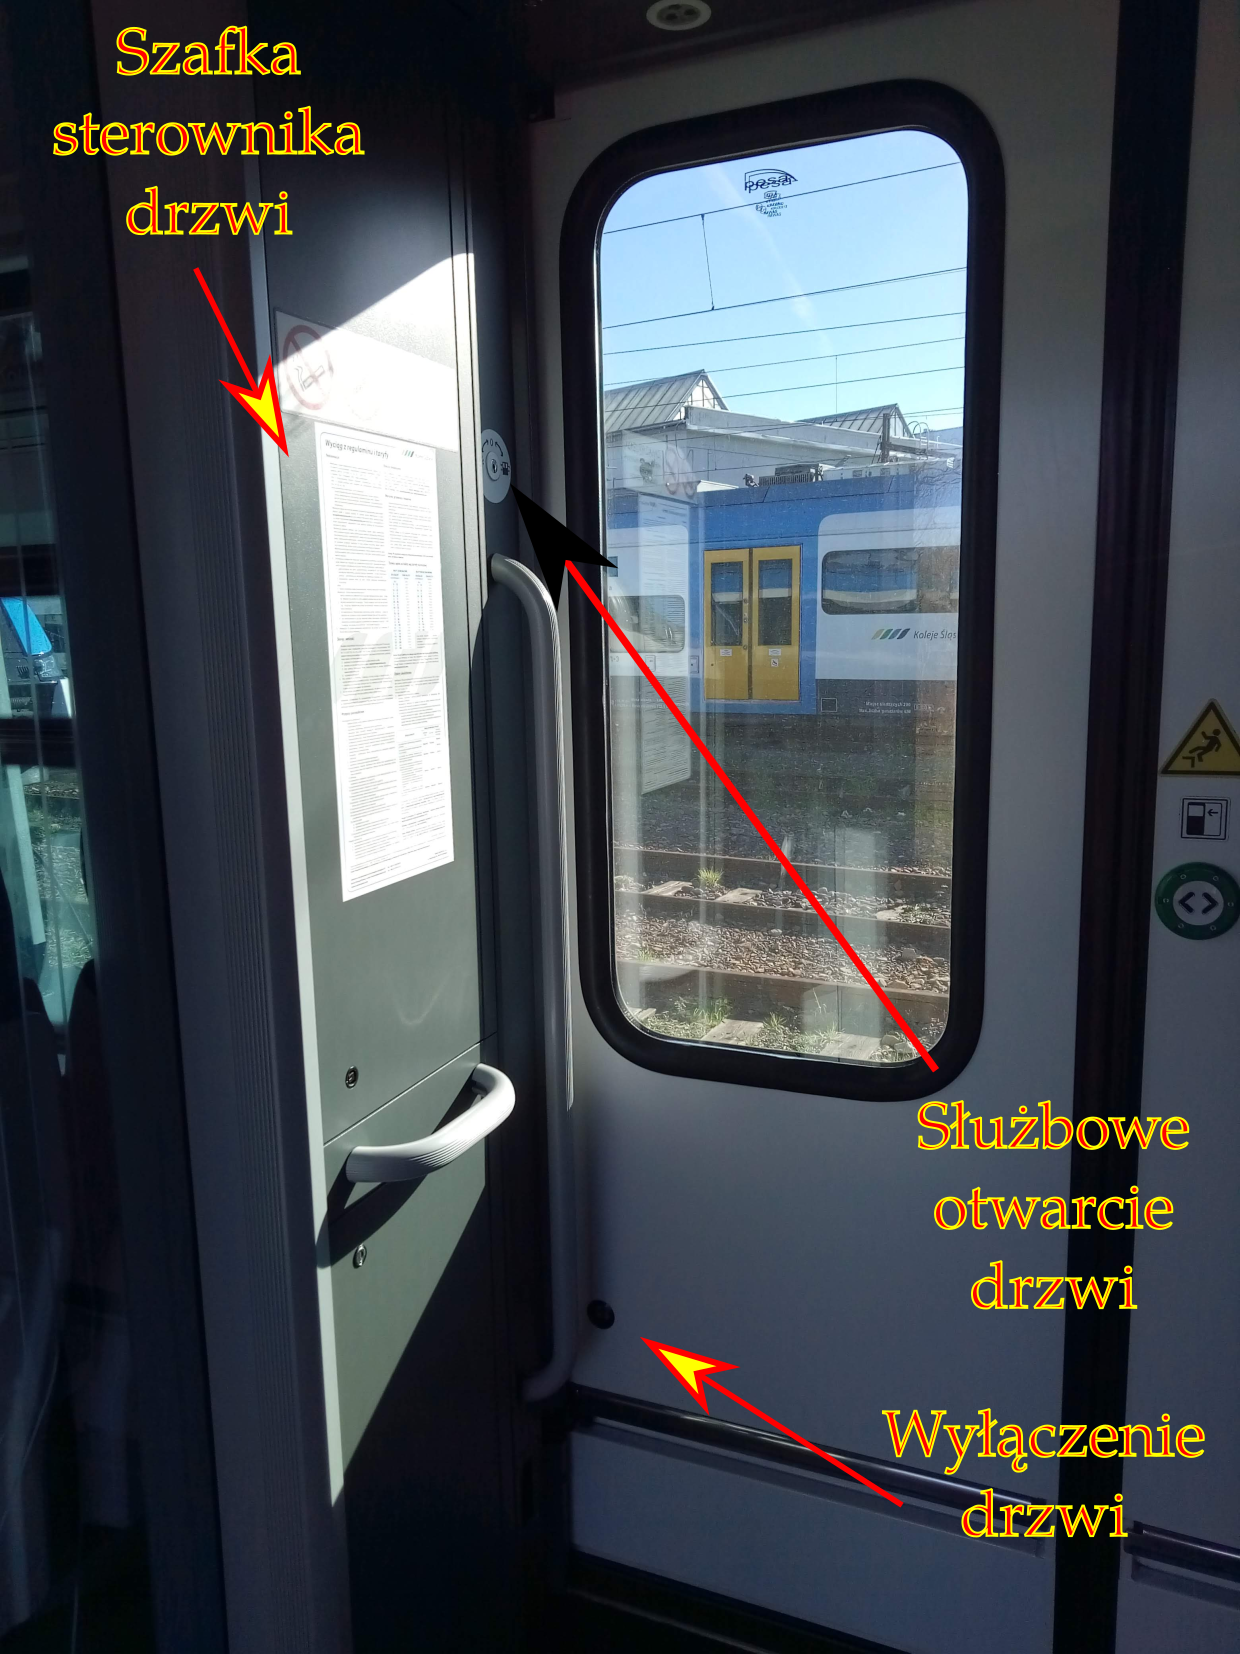
\includegraphics[width=4cm]{skryptkierownik-img/skryptkierownik-img049.png}}
		\subfloat{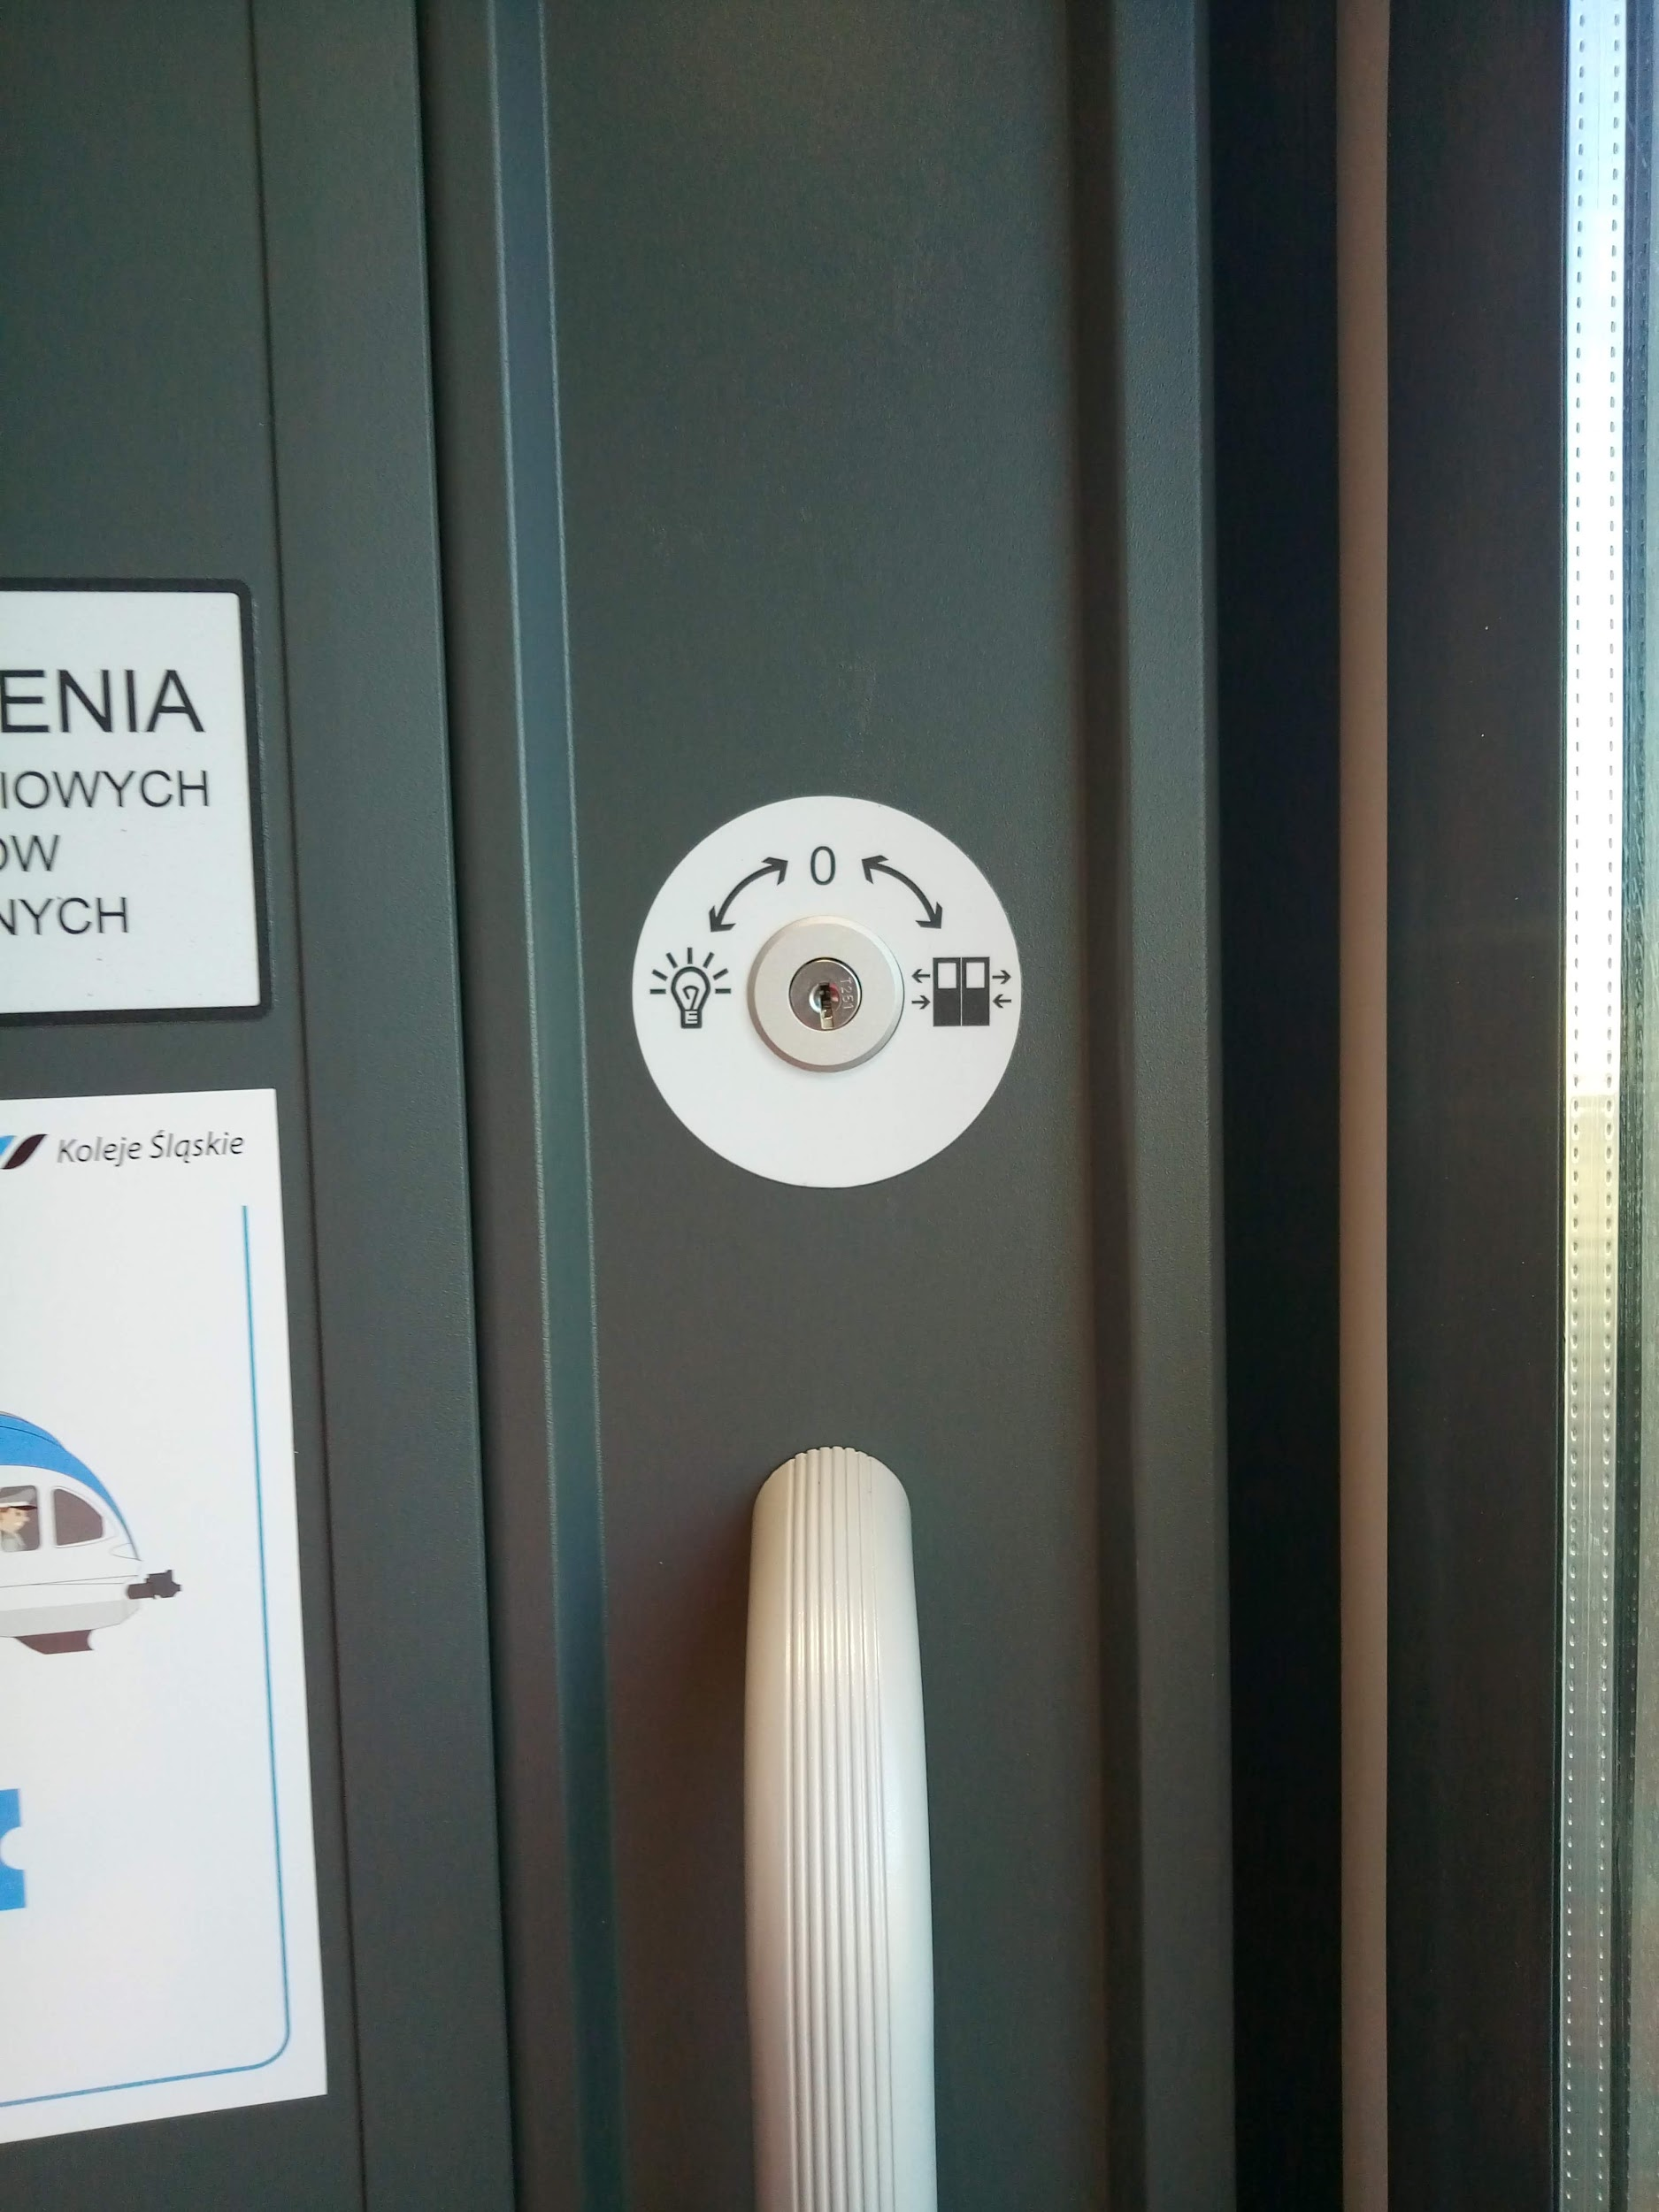
\includegraphics[width=4cm]{skryptkierownik-img/skryptkierownik-img050.jpg}}
		\subfloat{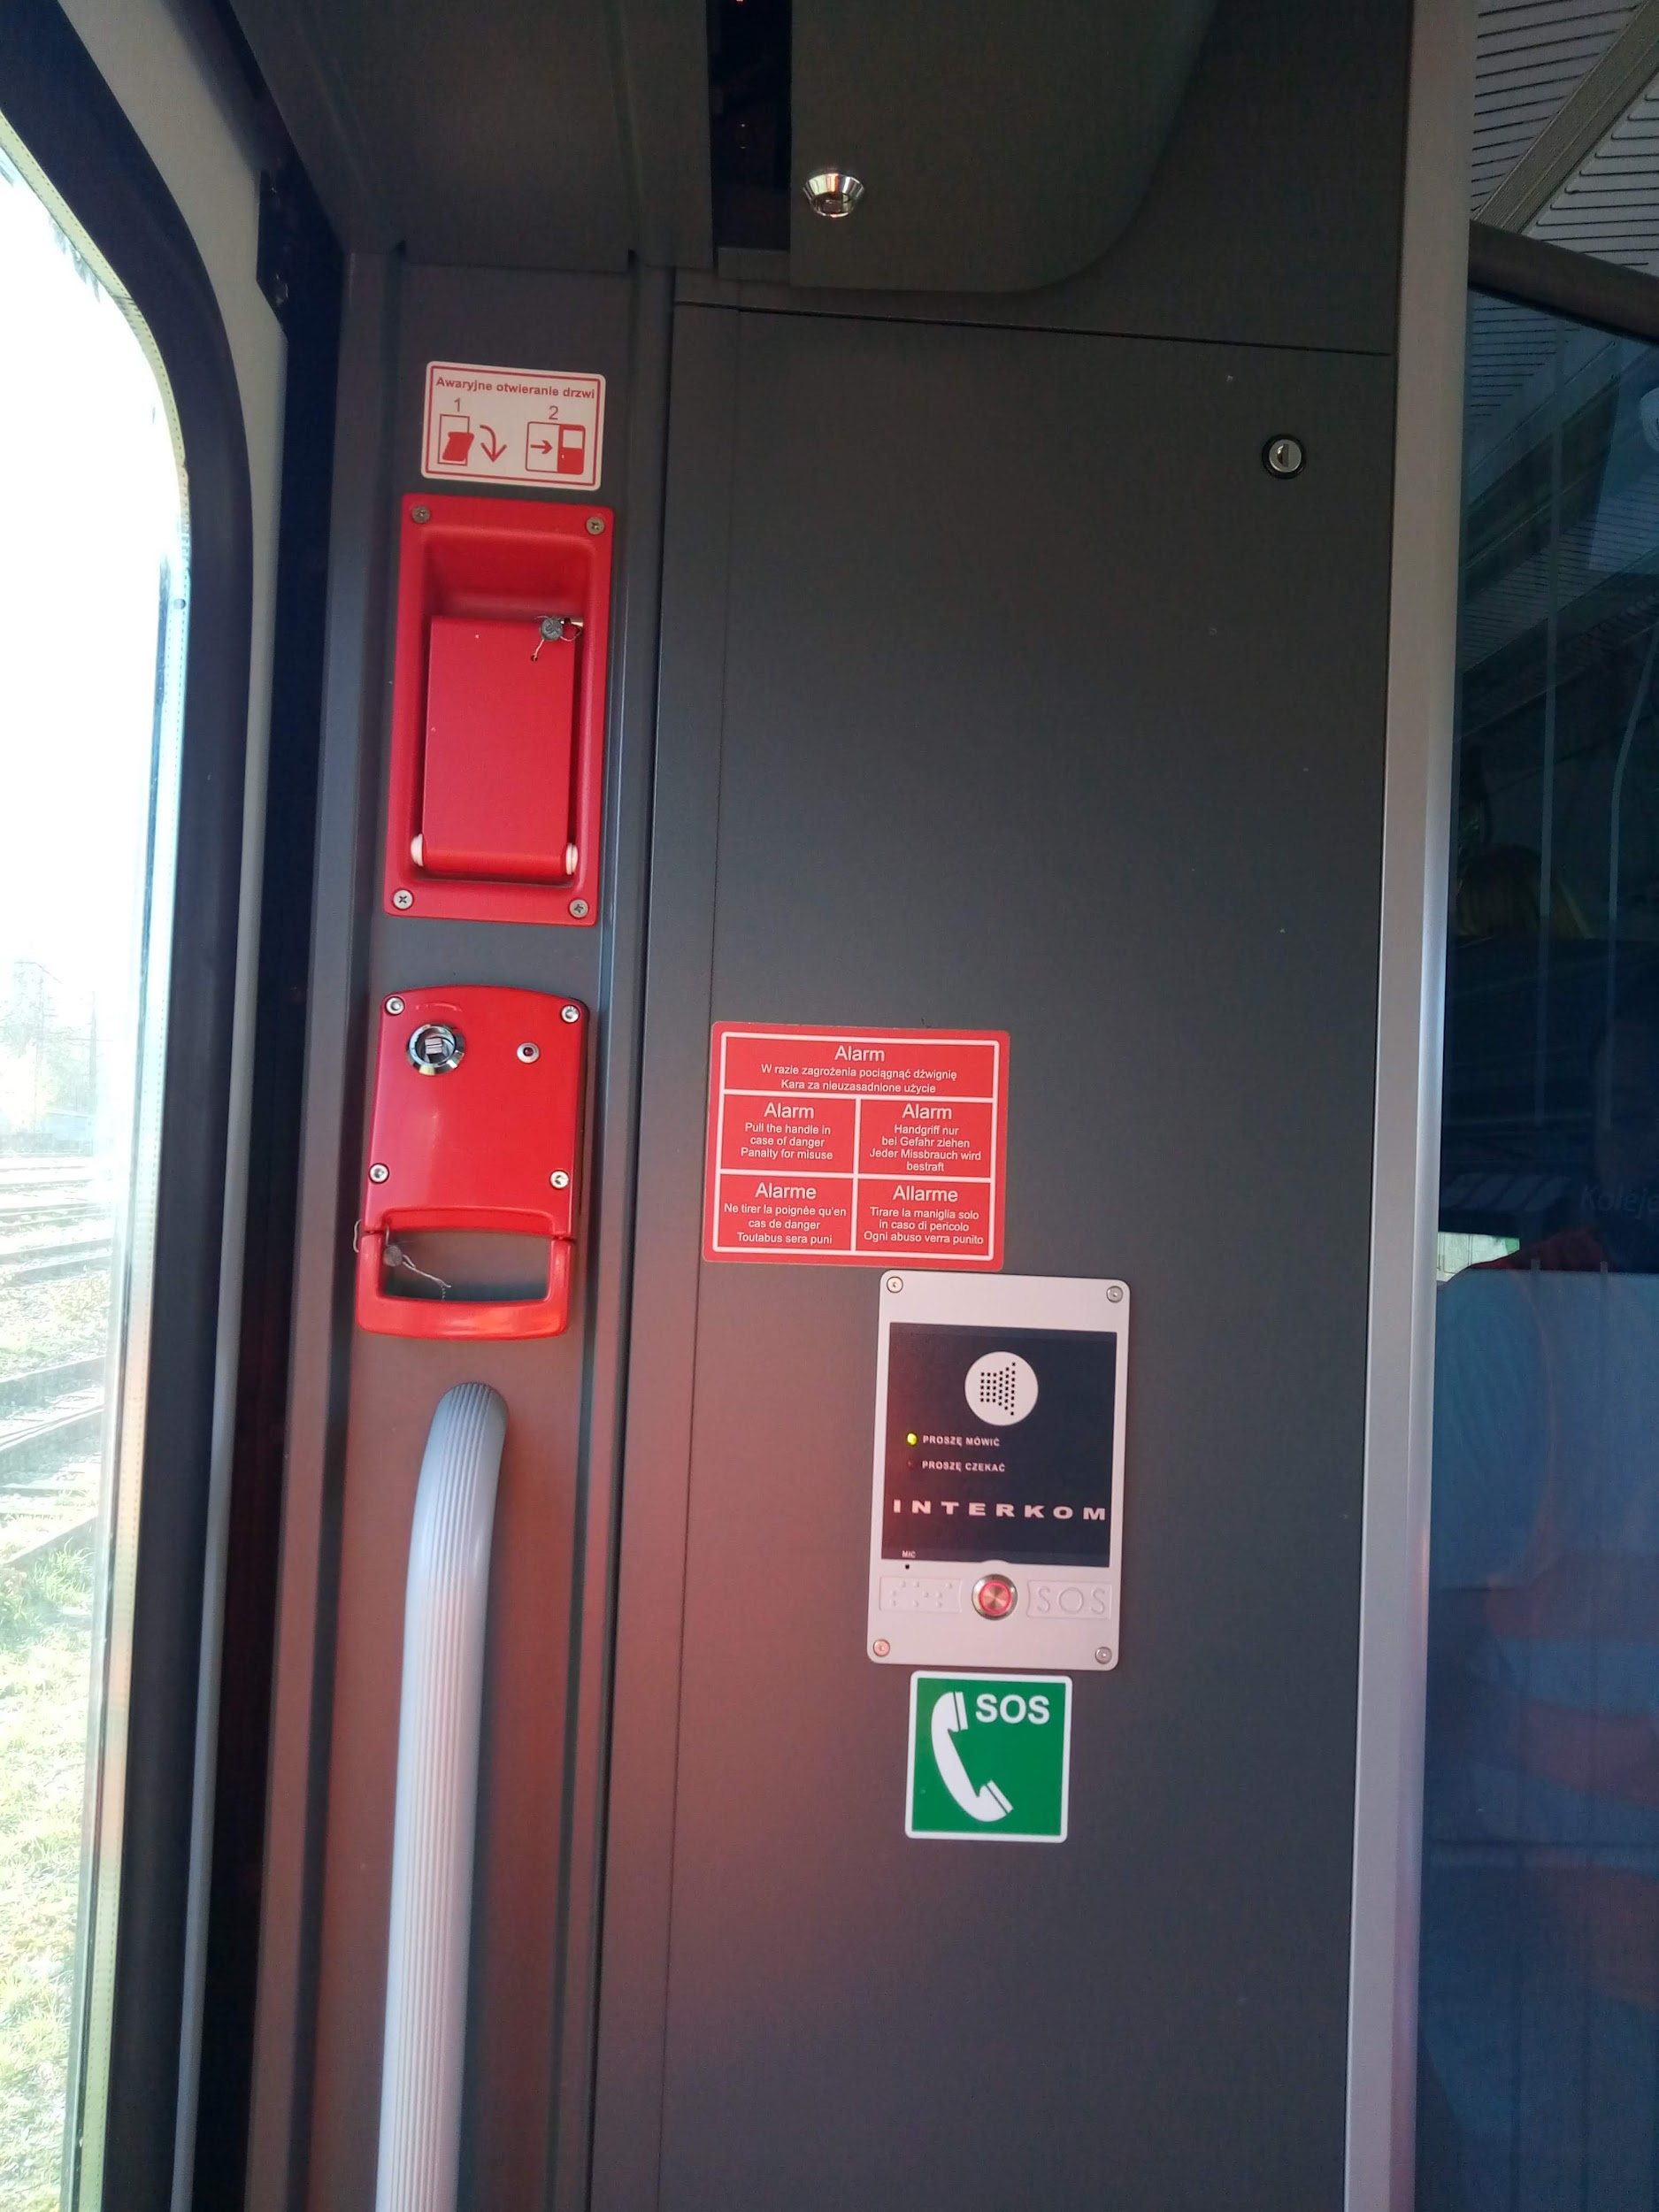
\includegraphics[width=4cm]{skryptkierownik-img/skryptkierownik-img051.jpg}}
		\caption{Lokalizacja urządzeń sterowania drzwi Elf2. W lewym portalu przełącznik otwierania służbowego drzwi, po stronie prawej Hamulec bezpieczeństwa i awaryjne otwieranie drzwi}
	\end{figure}

Po prawej stronie drzwi znajdują się hamulec bezpieczeństwa oraz dźwignia awaryjnego otwierania drzwi (bez zasilania). W celu zahamowania awaryjnego należu silnie pociągnąć rączkę hamulca w dół, aż do zerwania plomby. Dioda sygnalizuje użycie hamulca. Aby powrócić do pozycji zasadniczej, należy przekręcić kluczem konduktorskim, jednocześnie dociskając
rączkę hamulca ku górze. Poniżej po prawej stronie znajduje się interkom umożliwiający łączność z maszynistą.
W obudowie nad drzwiami wejściowymi do pojazdu znajduje się trzpień blokady drzwi, którego przekręcenie kluczem konduktorskim spowoduje wyłączenie napędu drzwi i ich zablokowanie. Pod obudową znajduje się sterownik, który można zresetować przyciskiem, jeśli drzwi chwilowo zachowują się niepoprawnie.

\begin{figure}
	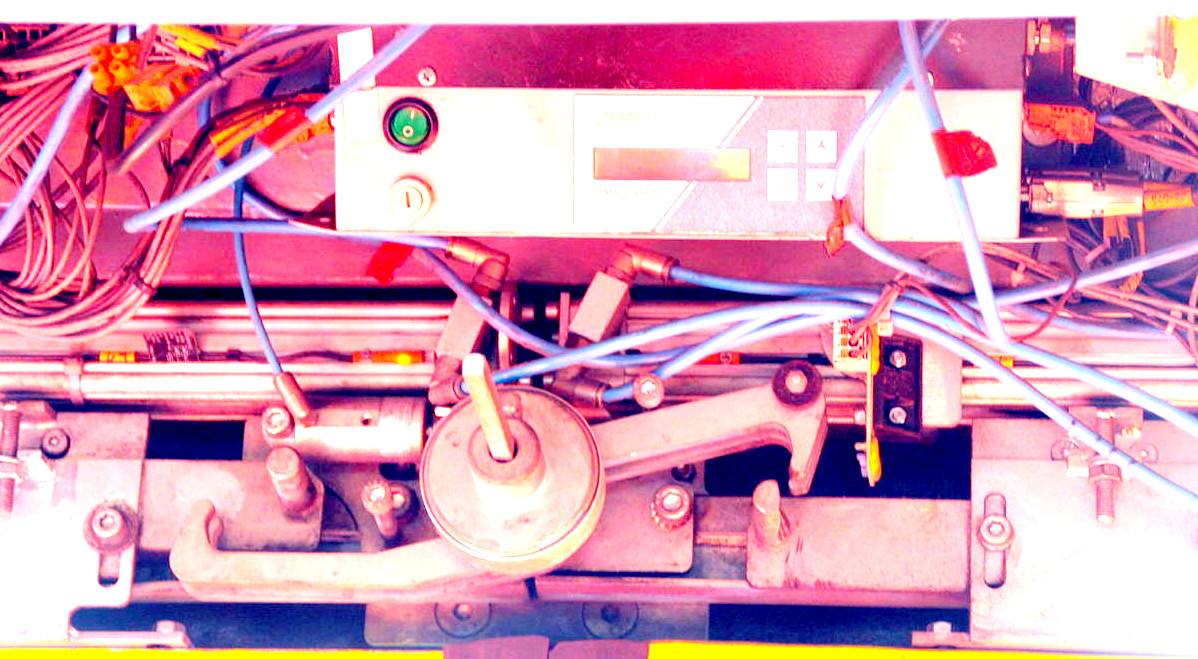
\includegraphics[width=12cm]{skryptkierownik-img/skryptkierownik-img059.jpg}
	\caption{Lokalizacja blokady i sterownika drzwi w pojazdach typu AKŚ}
\end{figure}
\begin{marginfigure}
	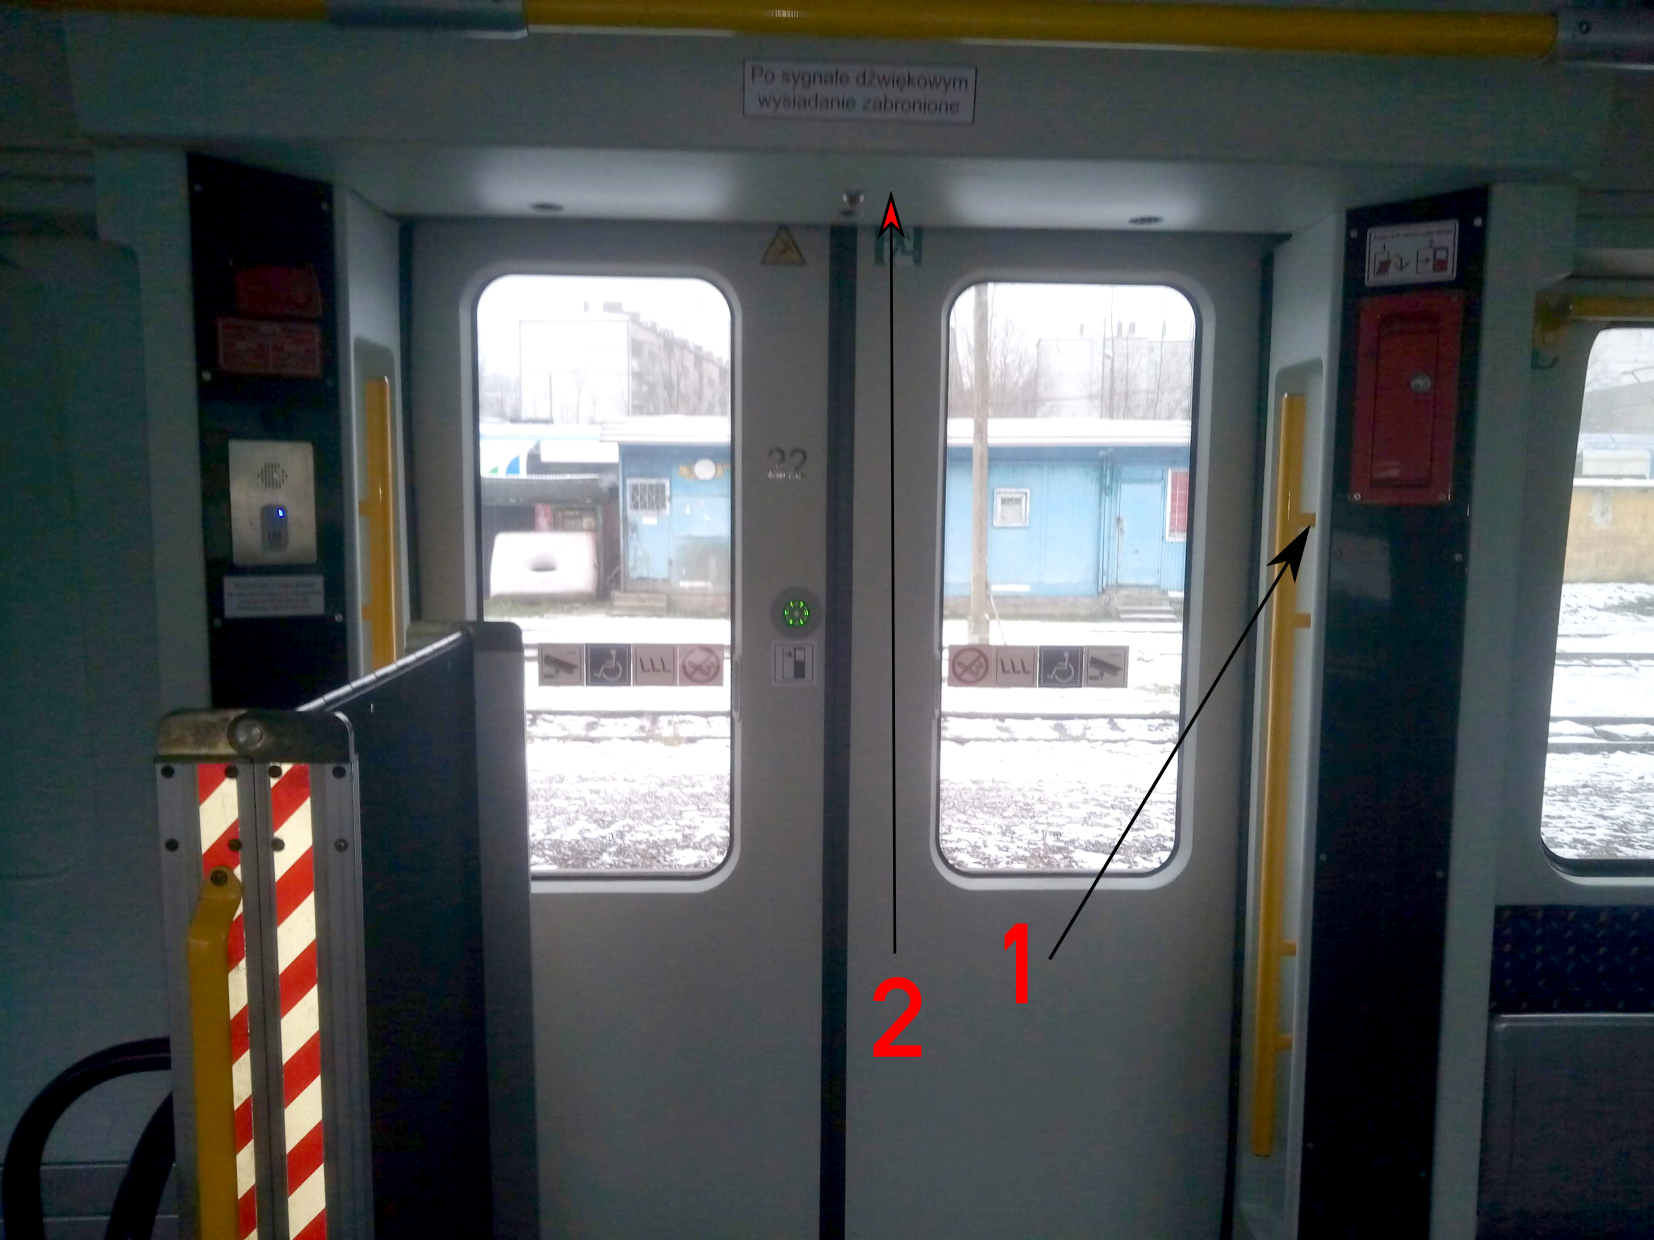
\includegraphics[width=5cm]{skryptkierownik-img/35we-drzwi.png}
	\caption{Układ elementów drzwi 35WE, cyfrą jeden oznaczone awaryjne otwieranie drzwi i wyłącznik mechanizmu, pod pokrywą oznaczoną cyfrą 2 znajduje się przełącznik resetu sterownika}
\end{marginfigure}

W pojeździe typu 35WE w prawym słupku portalu drzwi znajduje się dźwignia awaryjnego otwierania drzwi. W niej zabudowany jest zamek na klucz konduktorski który po wciśnięciu i przekręceniu powoduje wyłączenie i zablokowanie tych drzwi ze sterowania. Dodatkowo pod górną klapą, w środkowej części znajduje się wyłącznik sterownika drzwi, który w przypadku problemów należy przełączyć do drugiej pozycji na chwilę, a następnie przywrócić do pozycji podstawowej. Absolutnie nie wolno pozostawiać przełącznika w pozycji ''wyłączony''. 

\section{Światła końca pociągu}

W pojazdach serii Elf 2, oraz 35WE na wyposażeniu znajdują się przenośne, zasilane bateryjnie tarcze świateł końca pociągu. Przenośne światła końca pociągu znajdują się w wysuwanej szufladzie (Elf 2), albo w dolnej części prawej szafy (Impuls) w przedsionku kabiny sterującej A.

\begin{figure}
		\subfloat{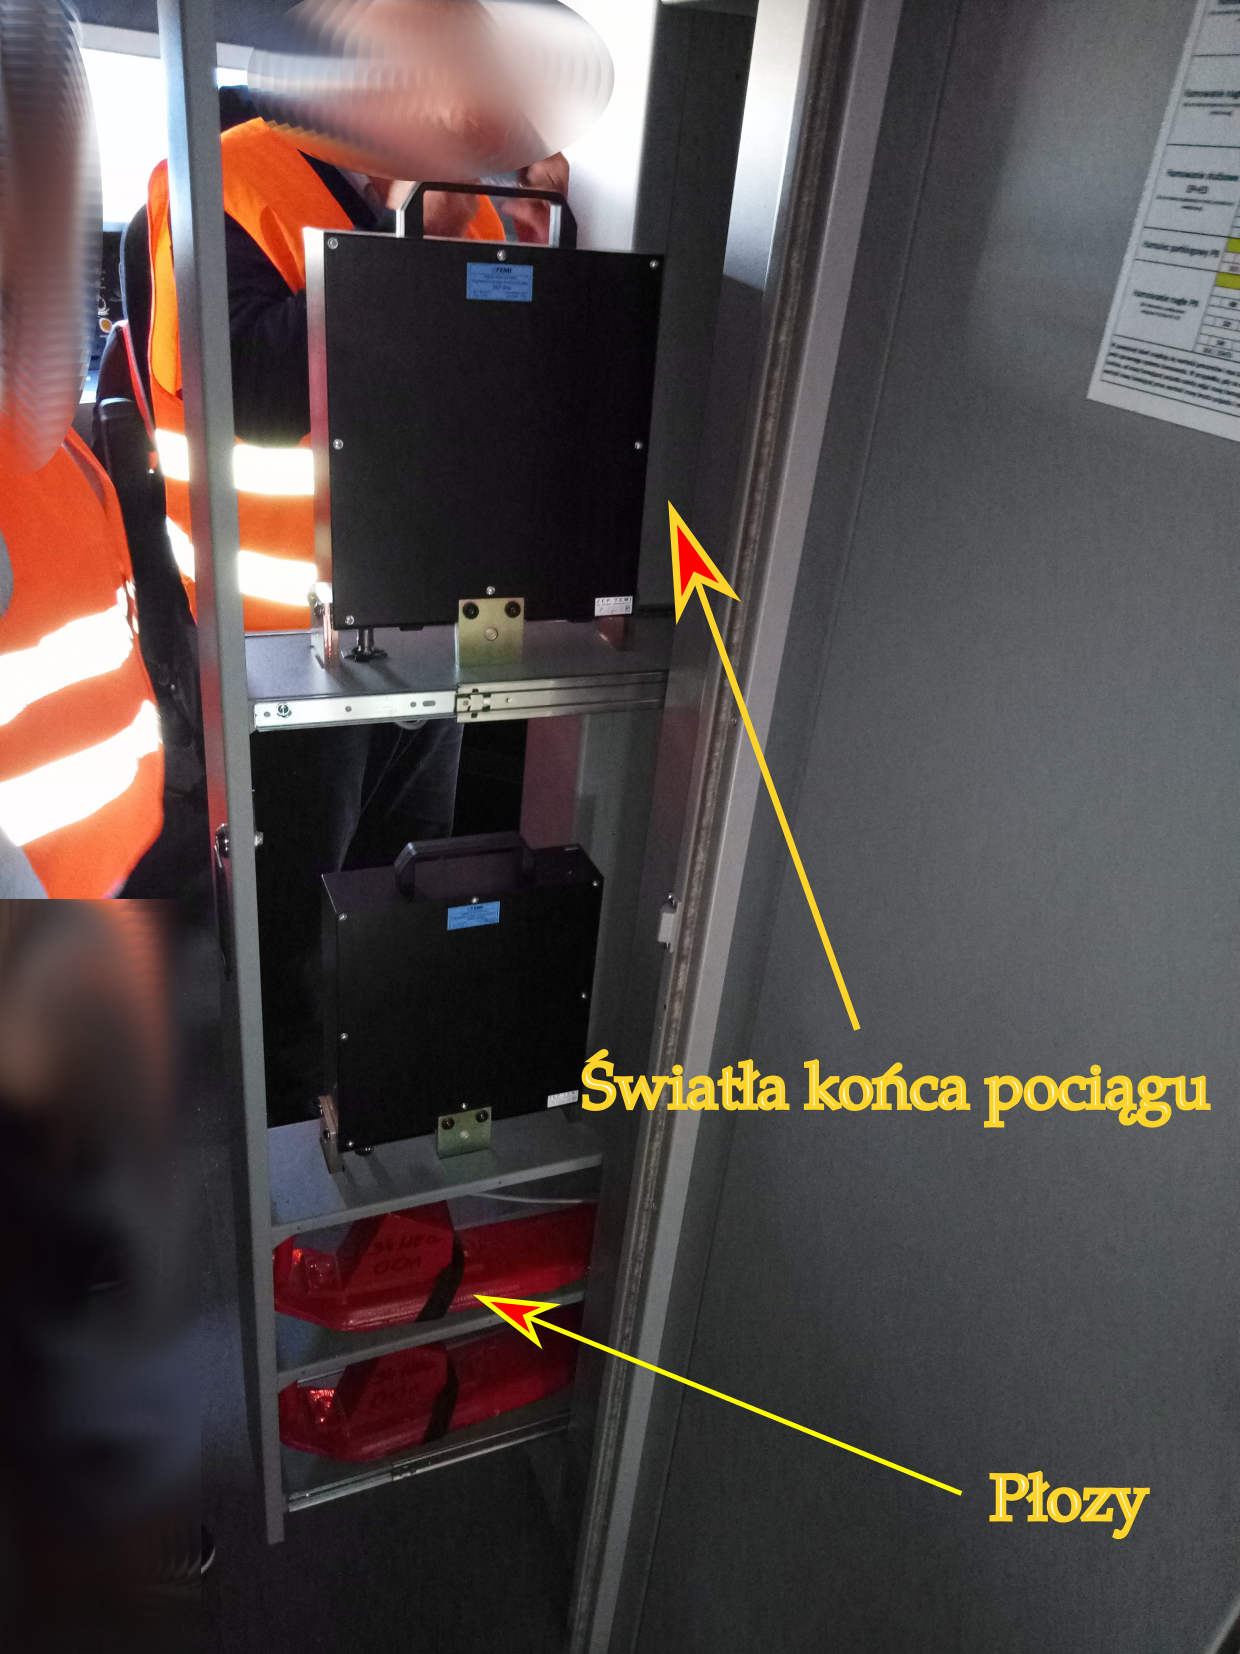
\includegraphics[width=6cm]{skryptkierownik-img/skryptkierownik-img042.png}}
		\subfloat{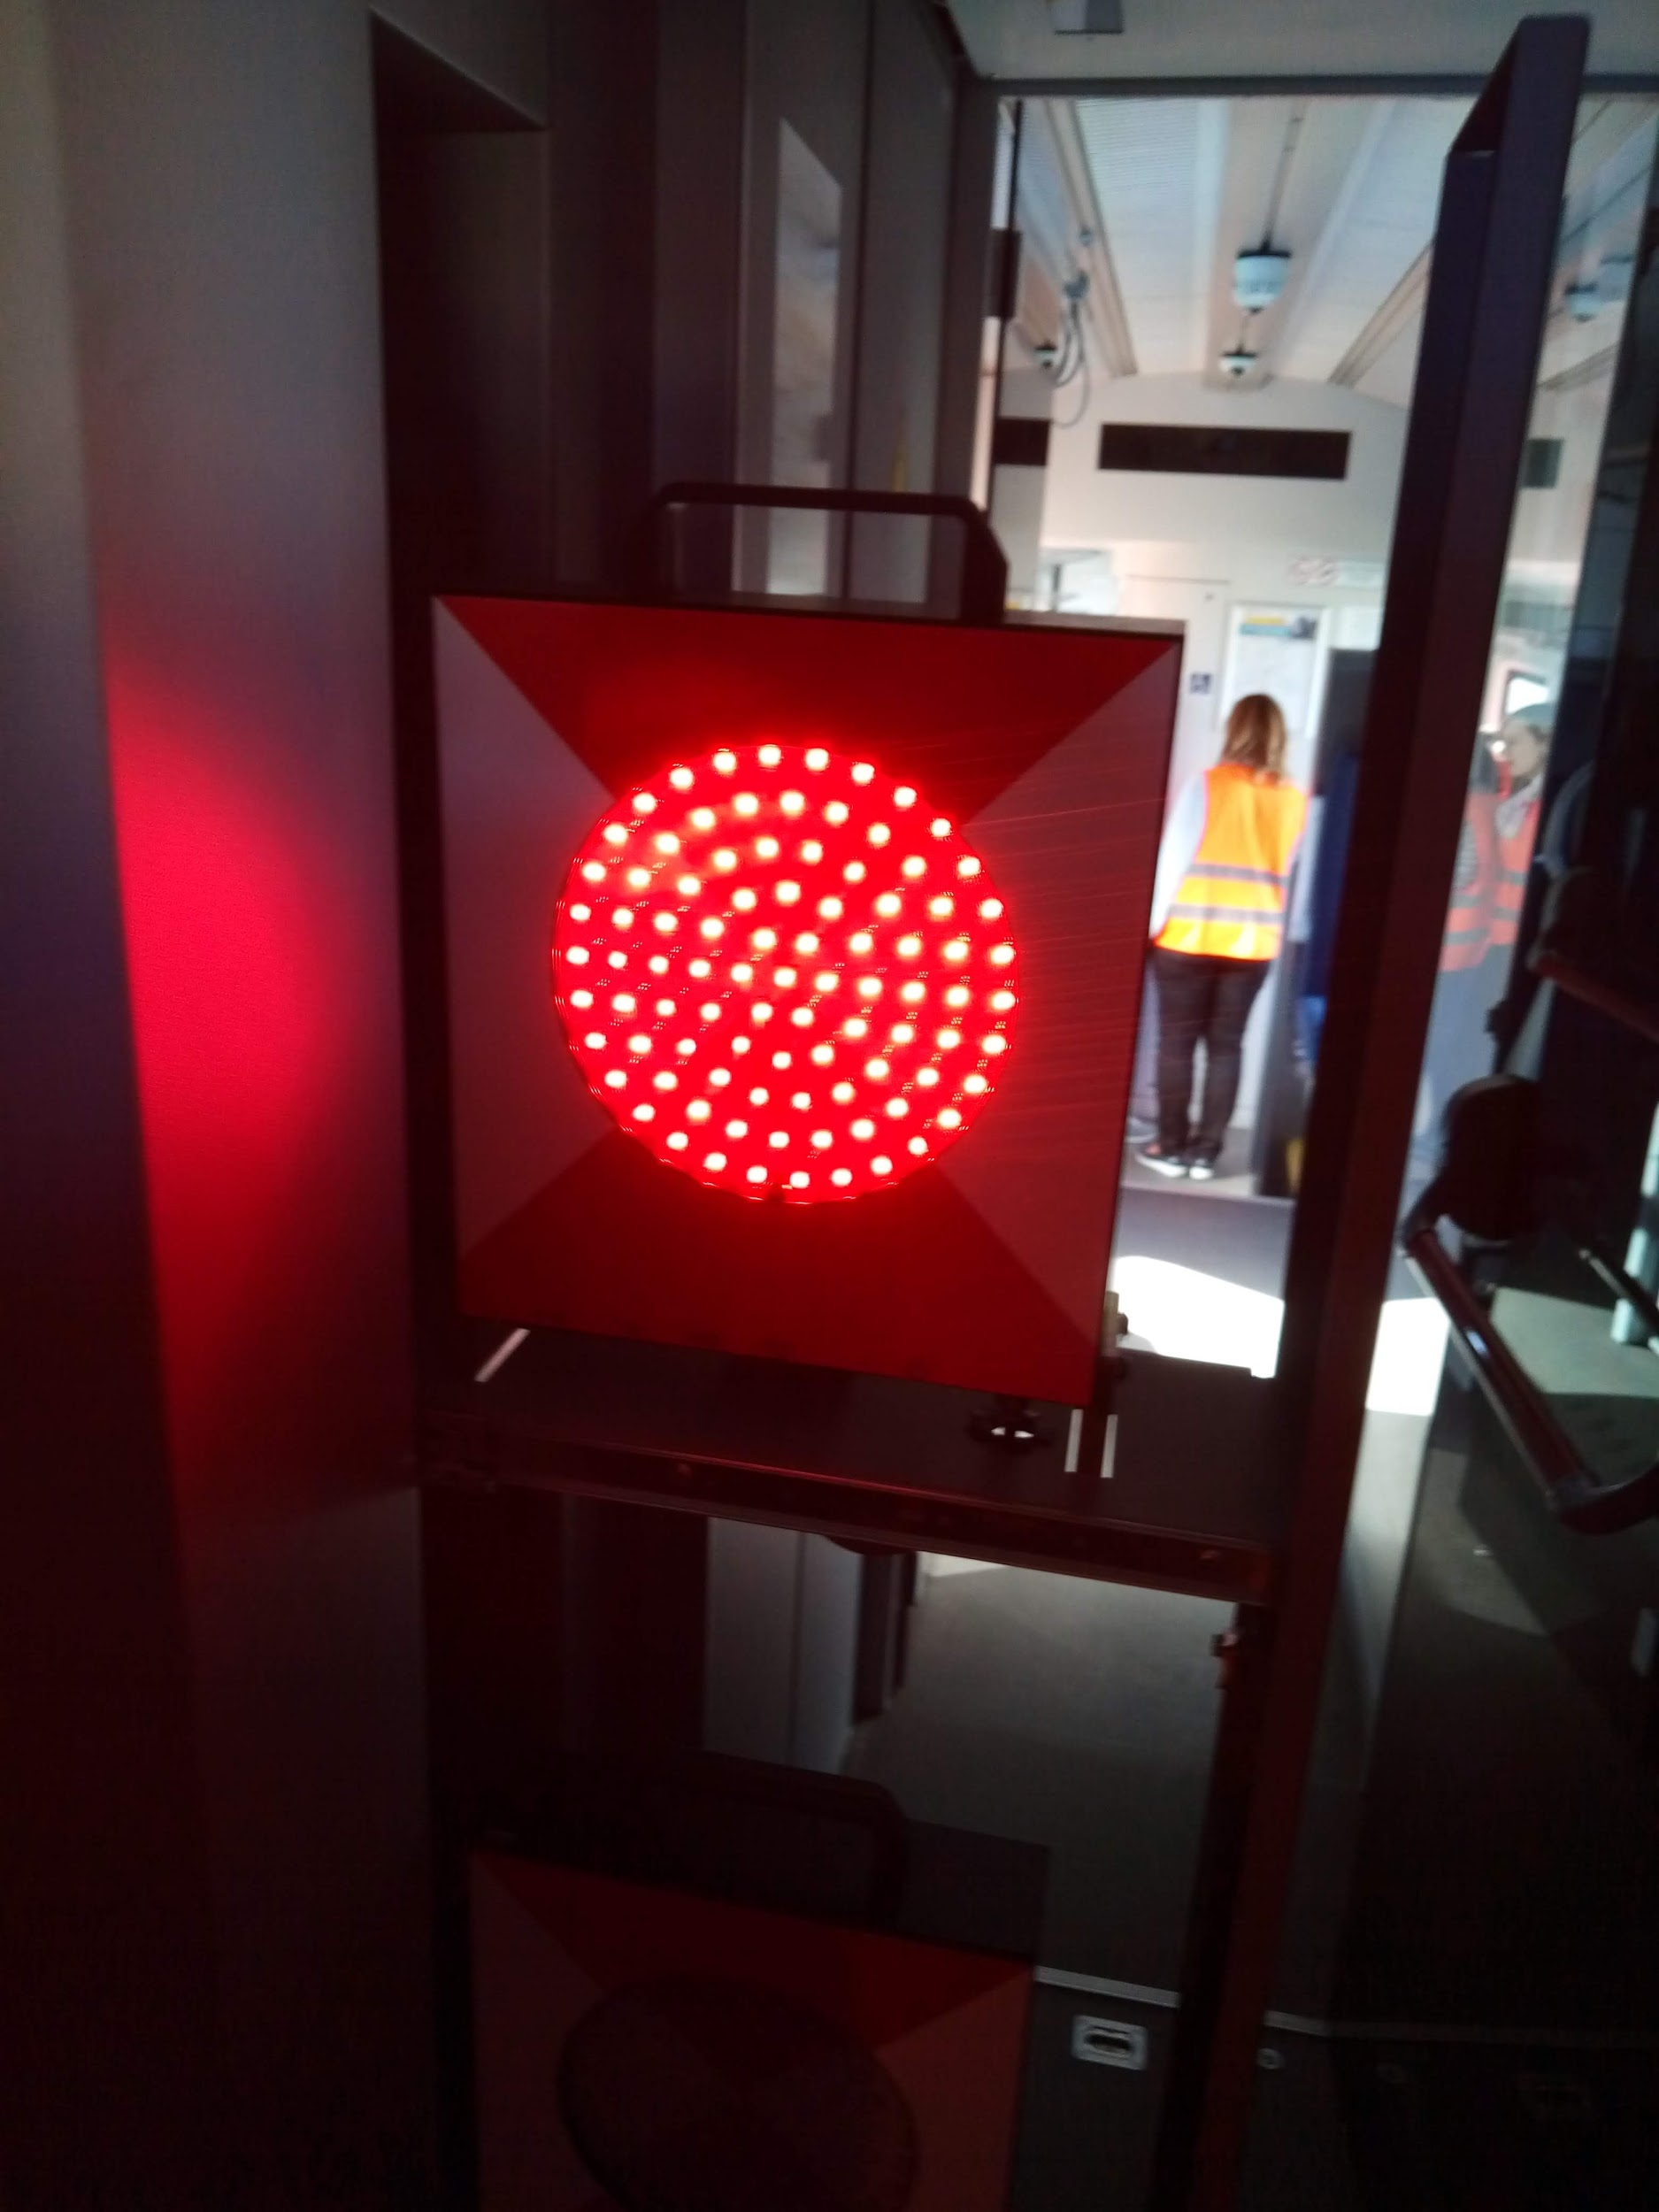
\includegraphics[width=6cm]{skryptkierownik-img/skryptkierownik-img043.jpg}}
		\caption{Szafa w przedsionku kabiny maszynisty, miejsce przechowywania świateł końca pociągu}
\end{figure}
Dodatkowo w pojazdach typu Elf 2, aby zamontować je na miejscu do tego przeznaczonym należy wykręcić kluczem konduktorskim śrubę zabezpieczającą, a następnie wysunąć zaślepkę, a potem umieścić w tym miejscu wspornik świateł. Następnie we wsporniku umieścić światło. W pozostałych pojazdach tarcze sygnałowe końca pociągu montuje się w stałym wsporniku, na czole.

\begin{figure}
\subfloat{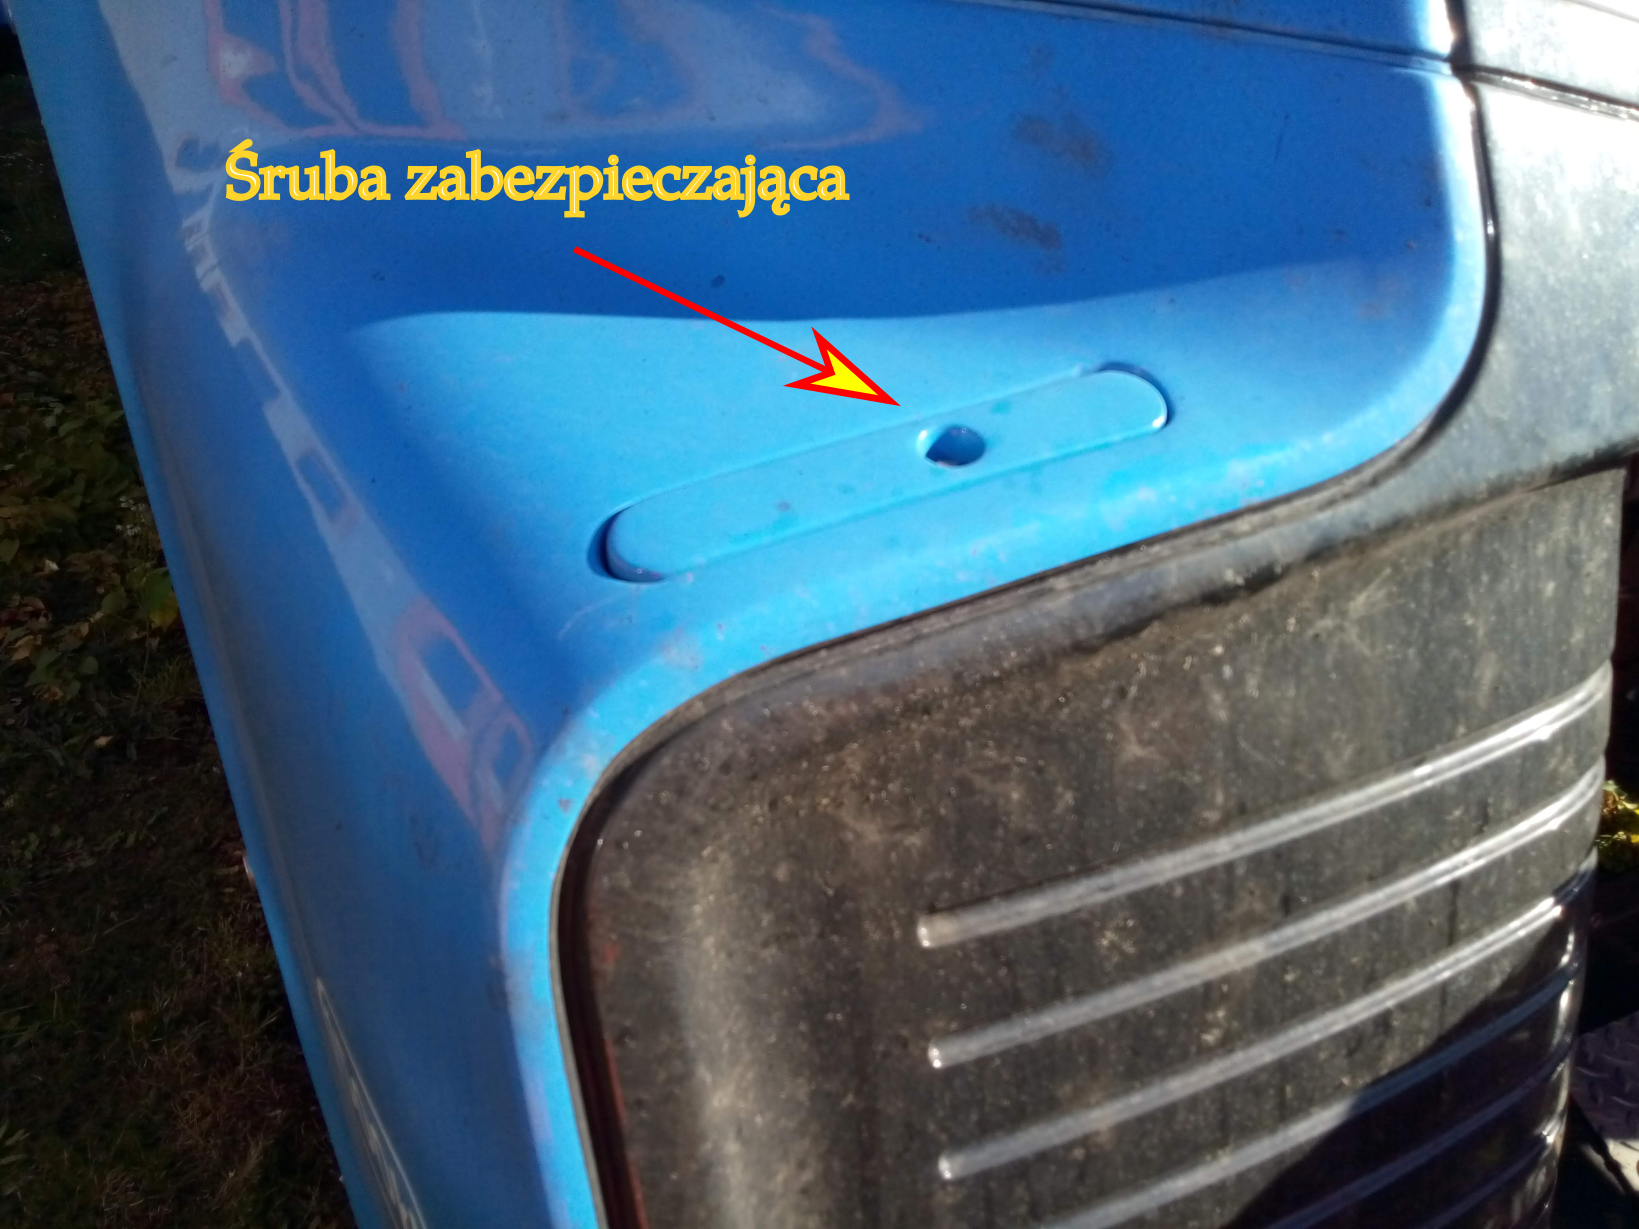
\includegraphics[width=6cm]{skryptkierownik-img/skryptkierownik-img044.png}}
\subfloat{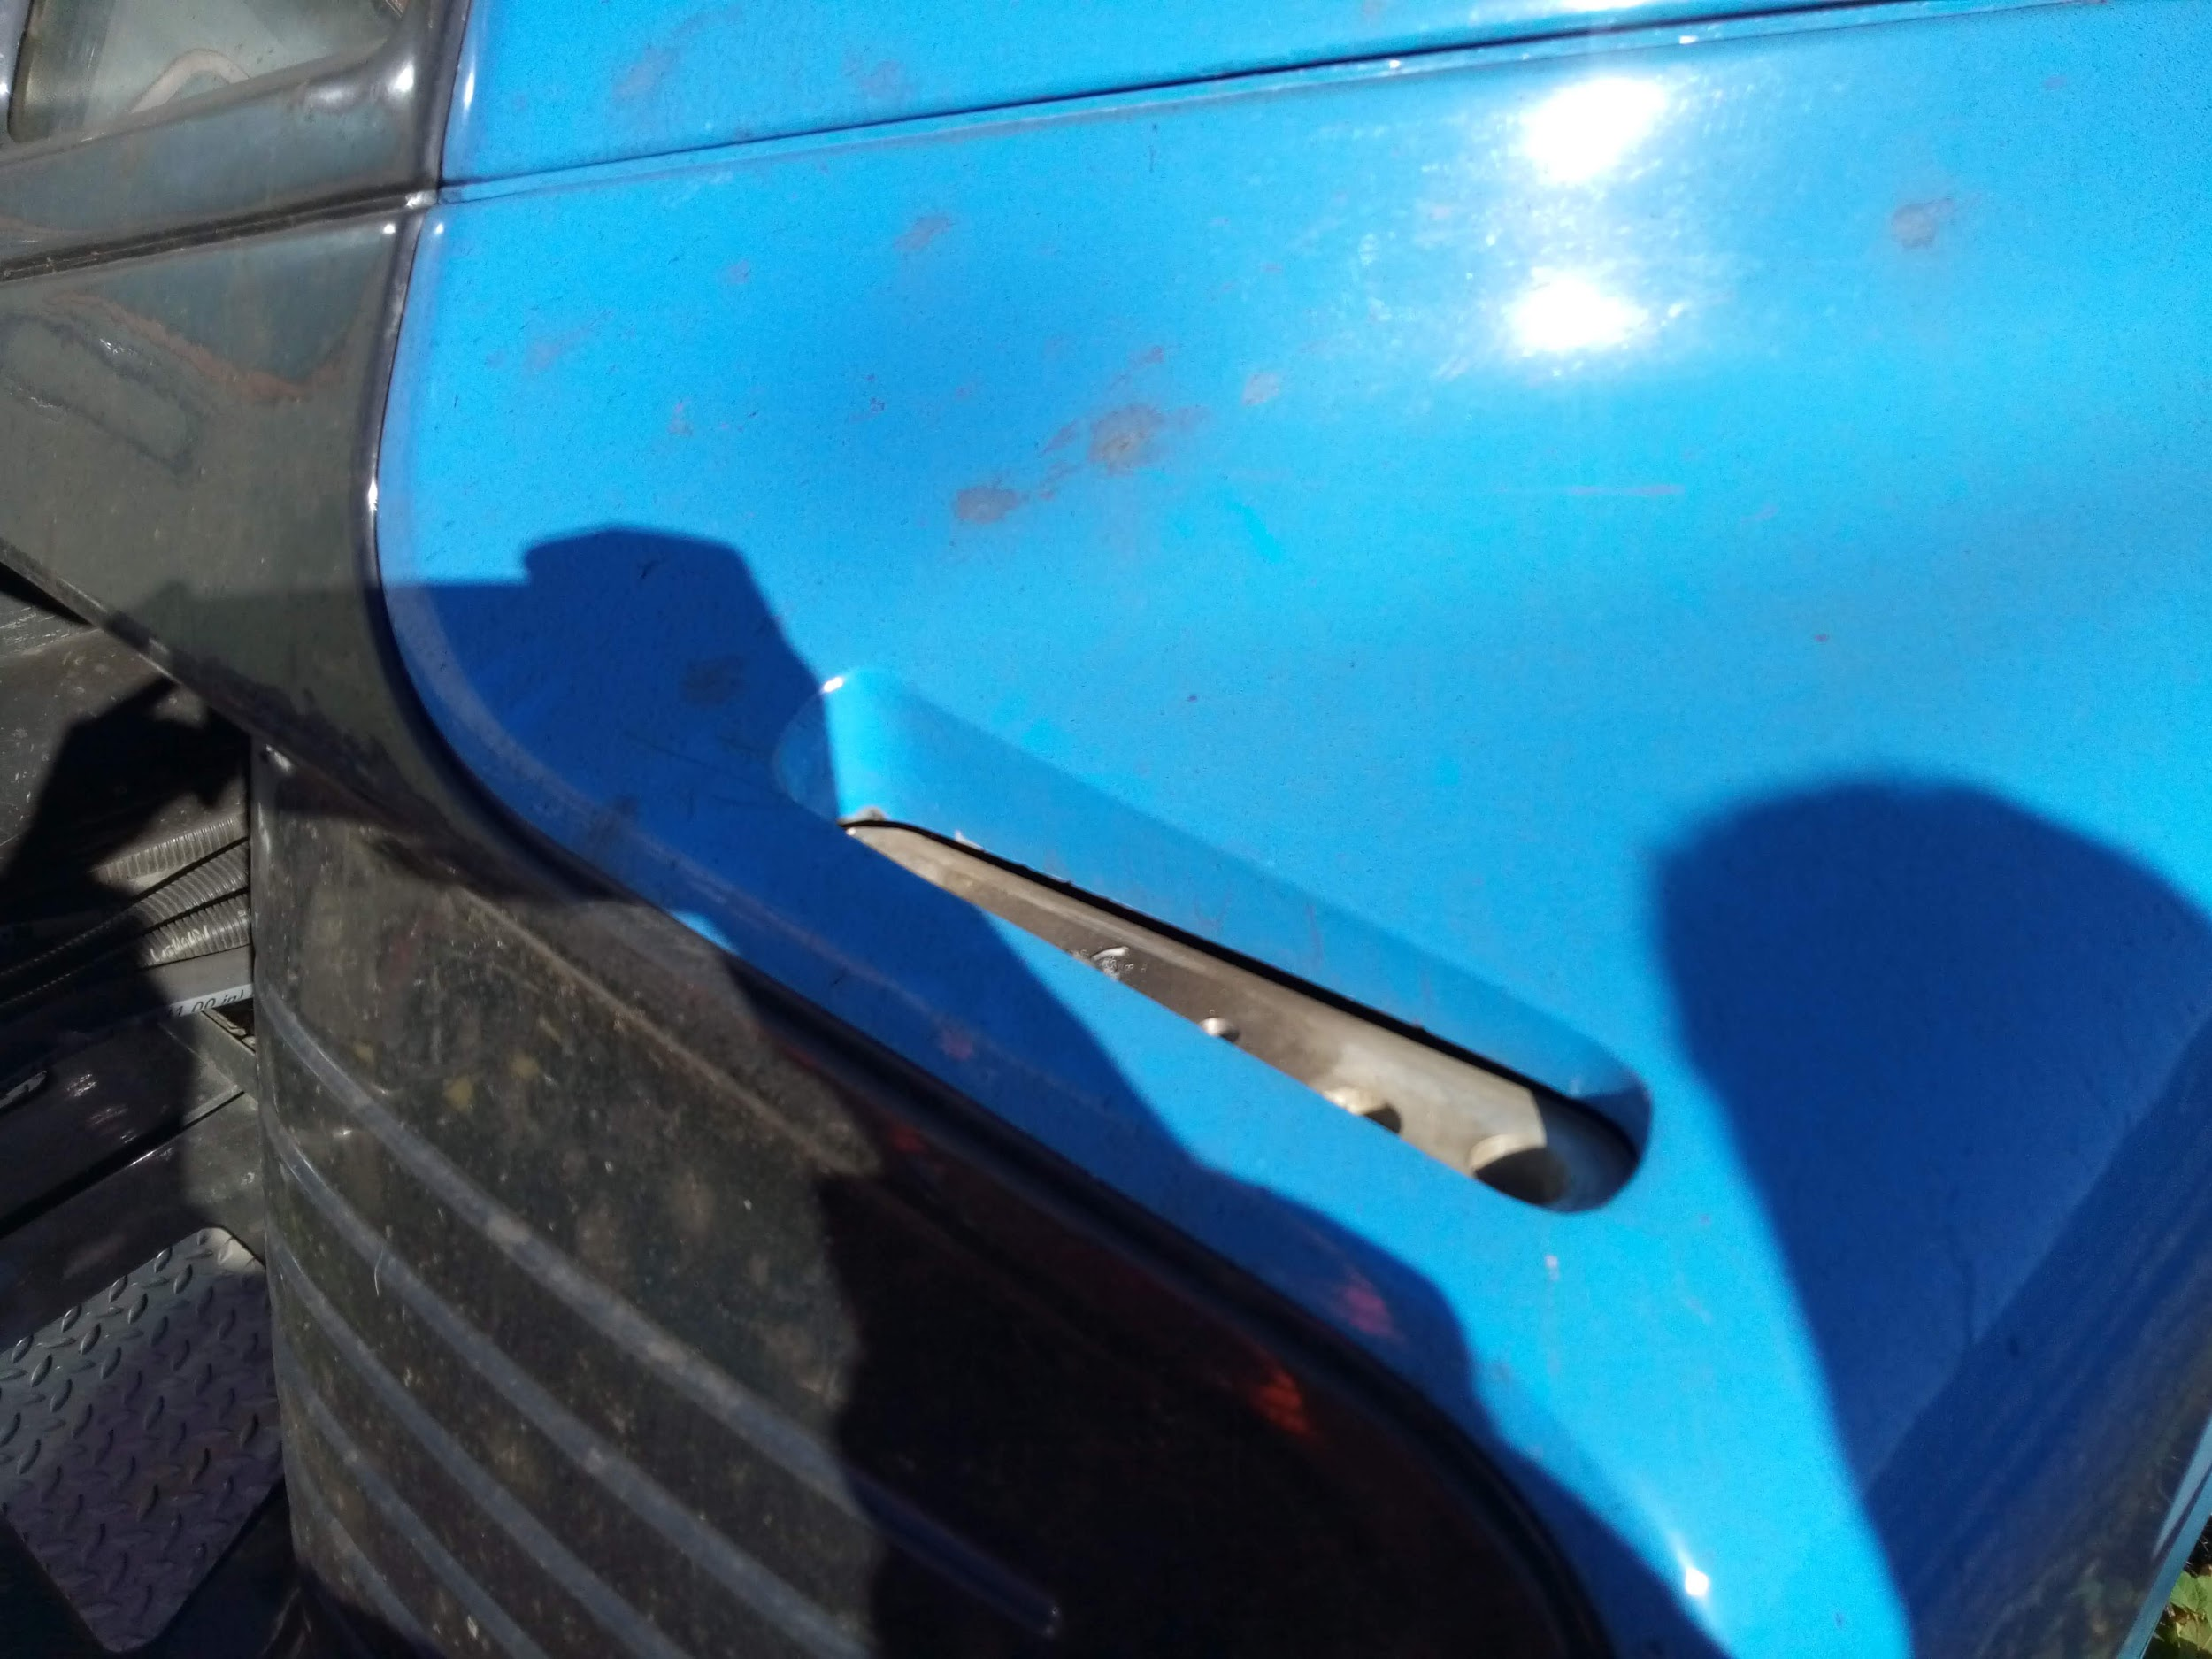
\includegraphics[width=6cm]{skryptkierownik-img/skryptkierownik-img045.jpg}}\\
\subfloat{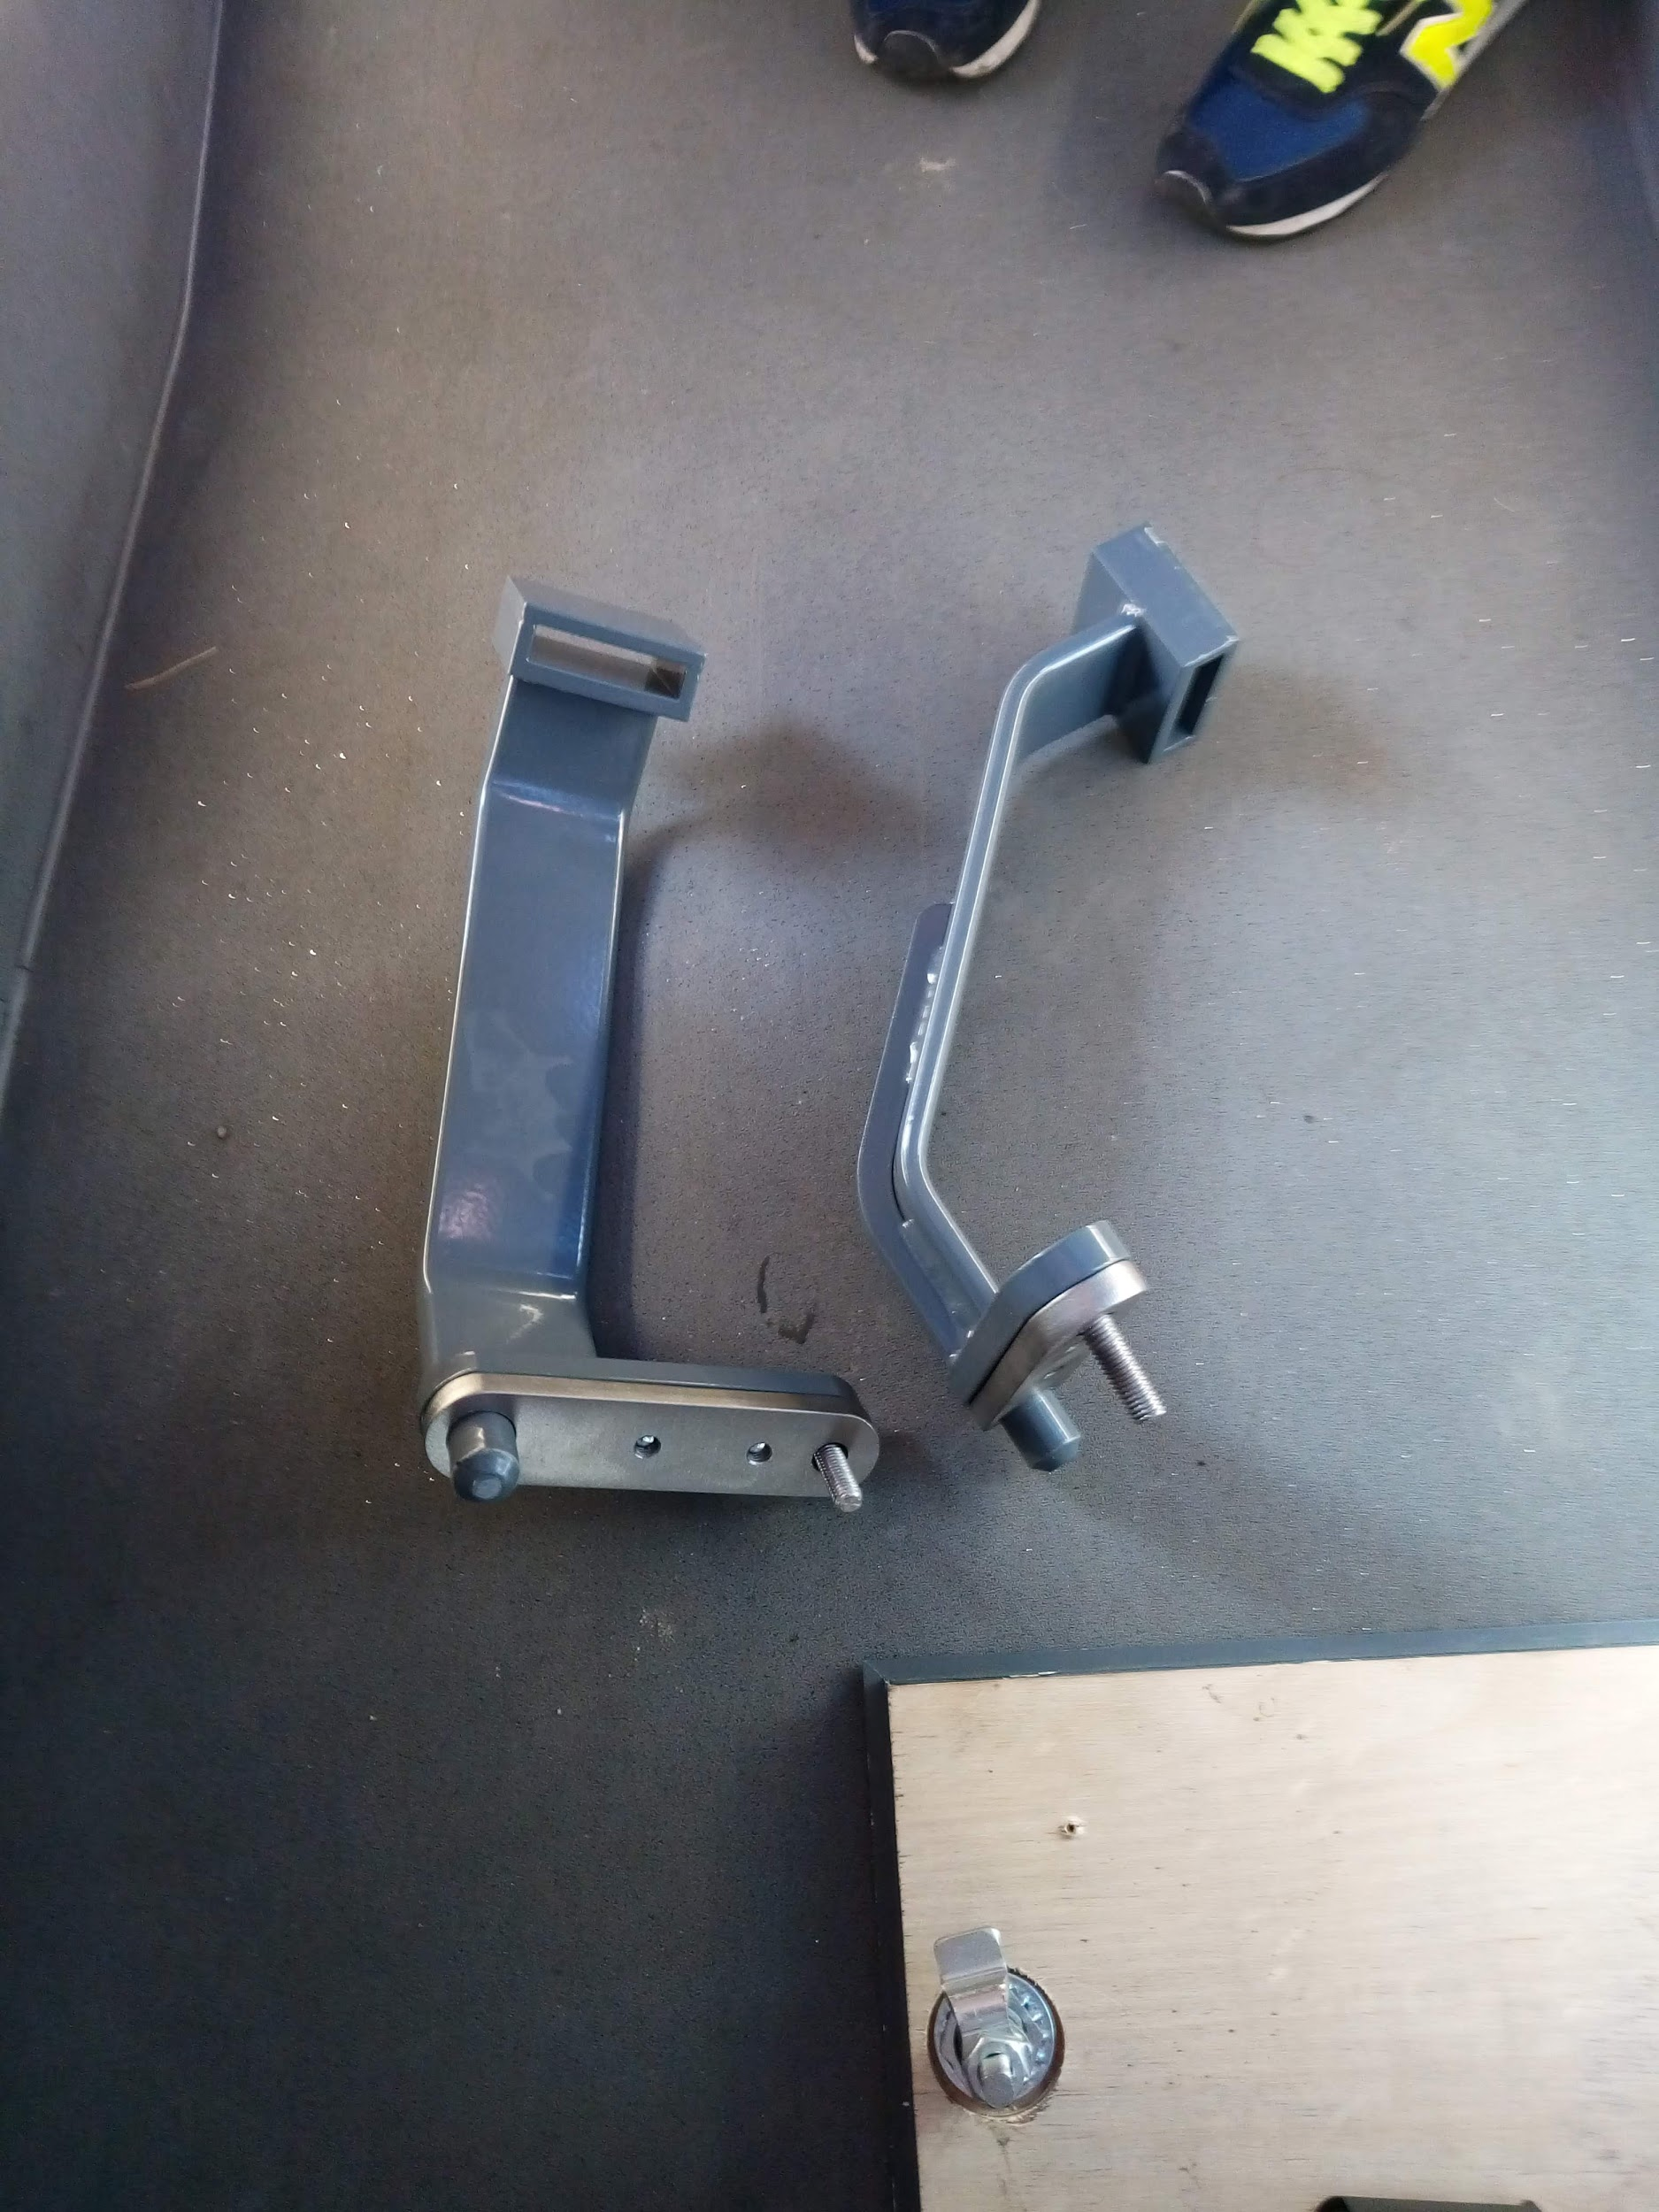
\includegraphics[width=6cm]{skryptkierownik-img/skryptkierownik-img046.jpg}}
\subfloat{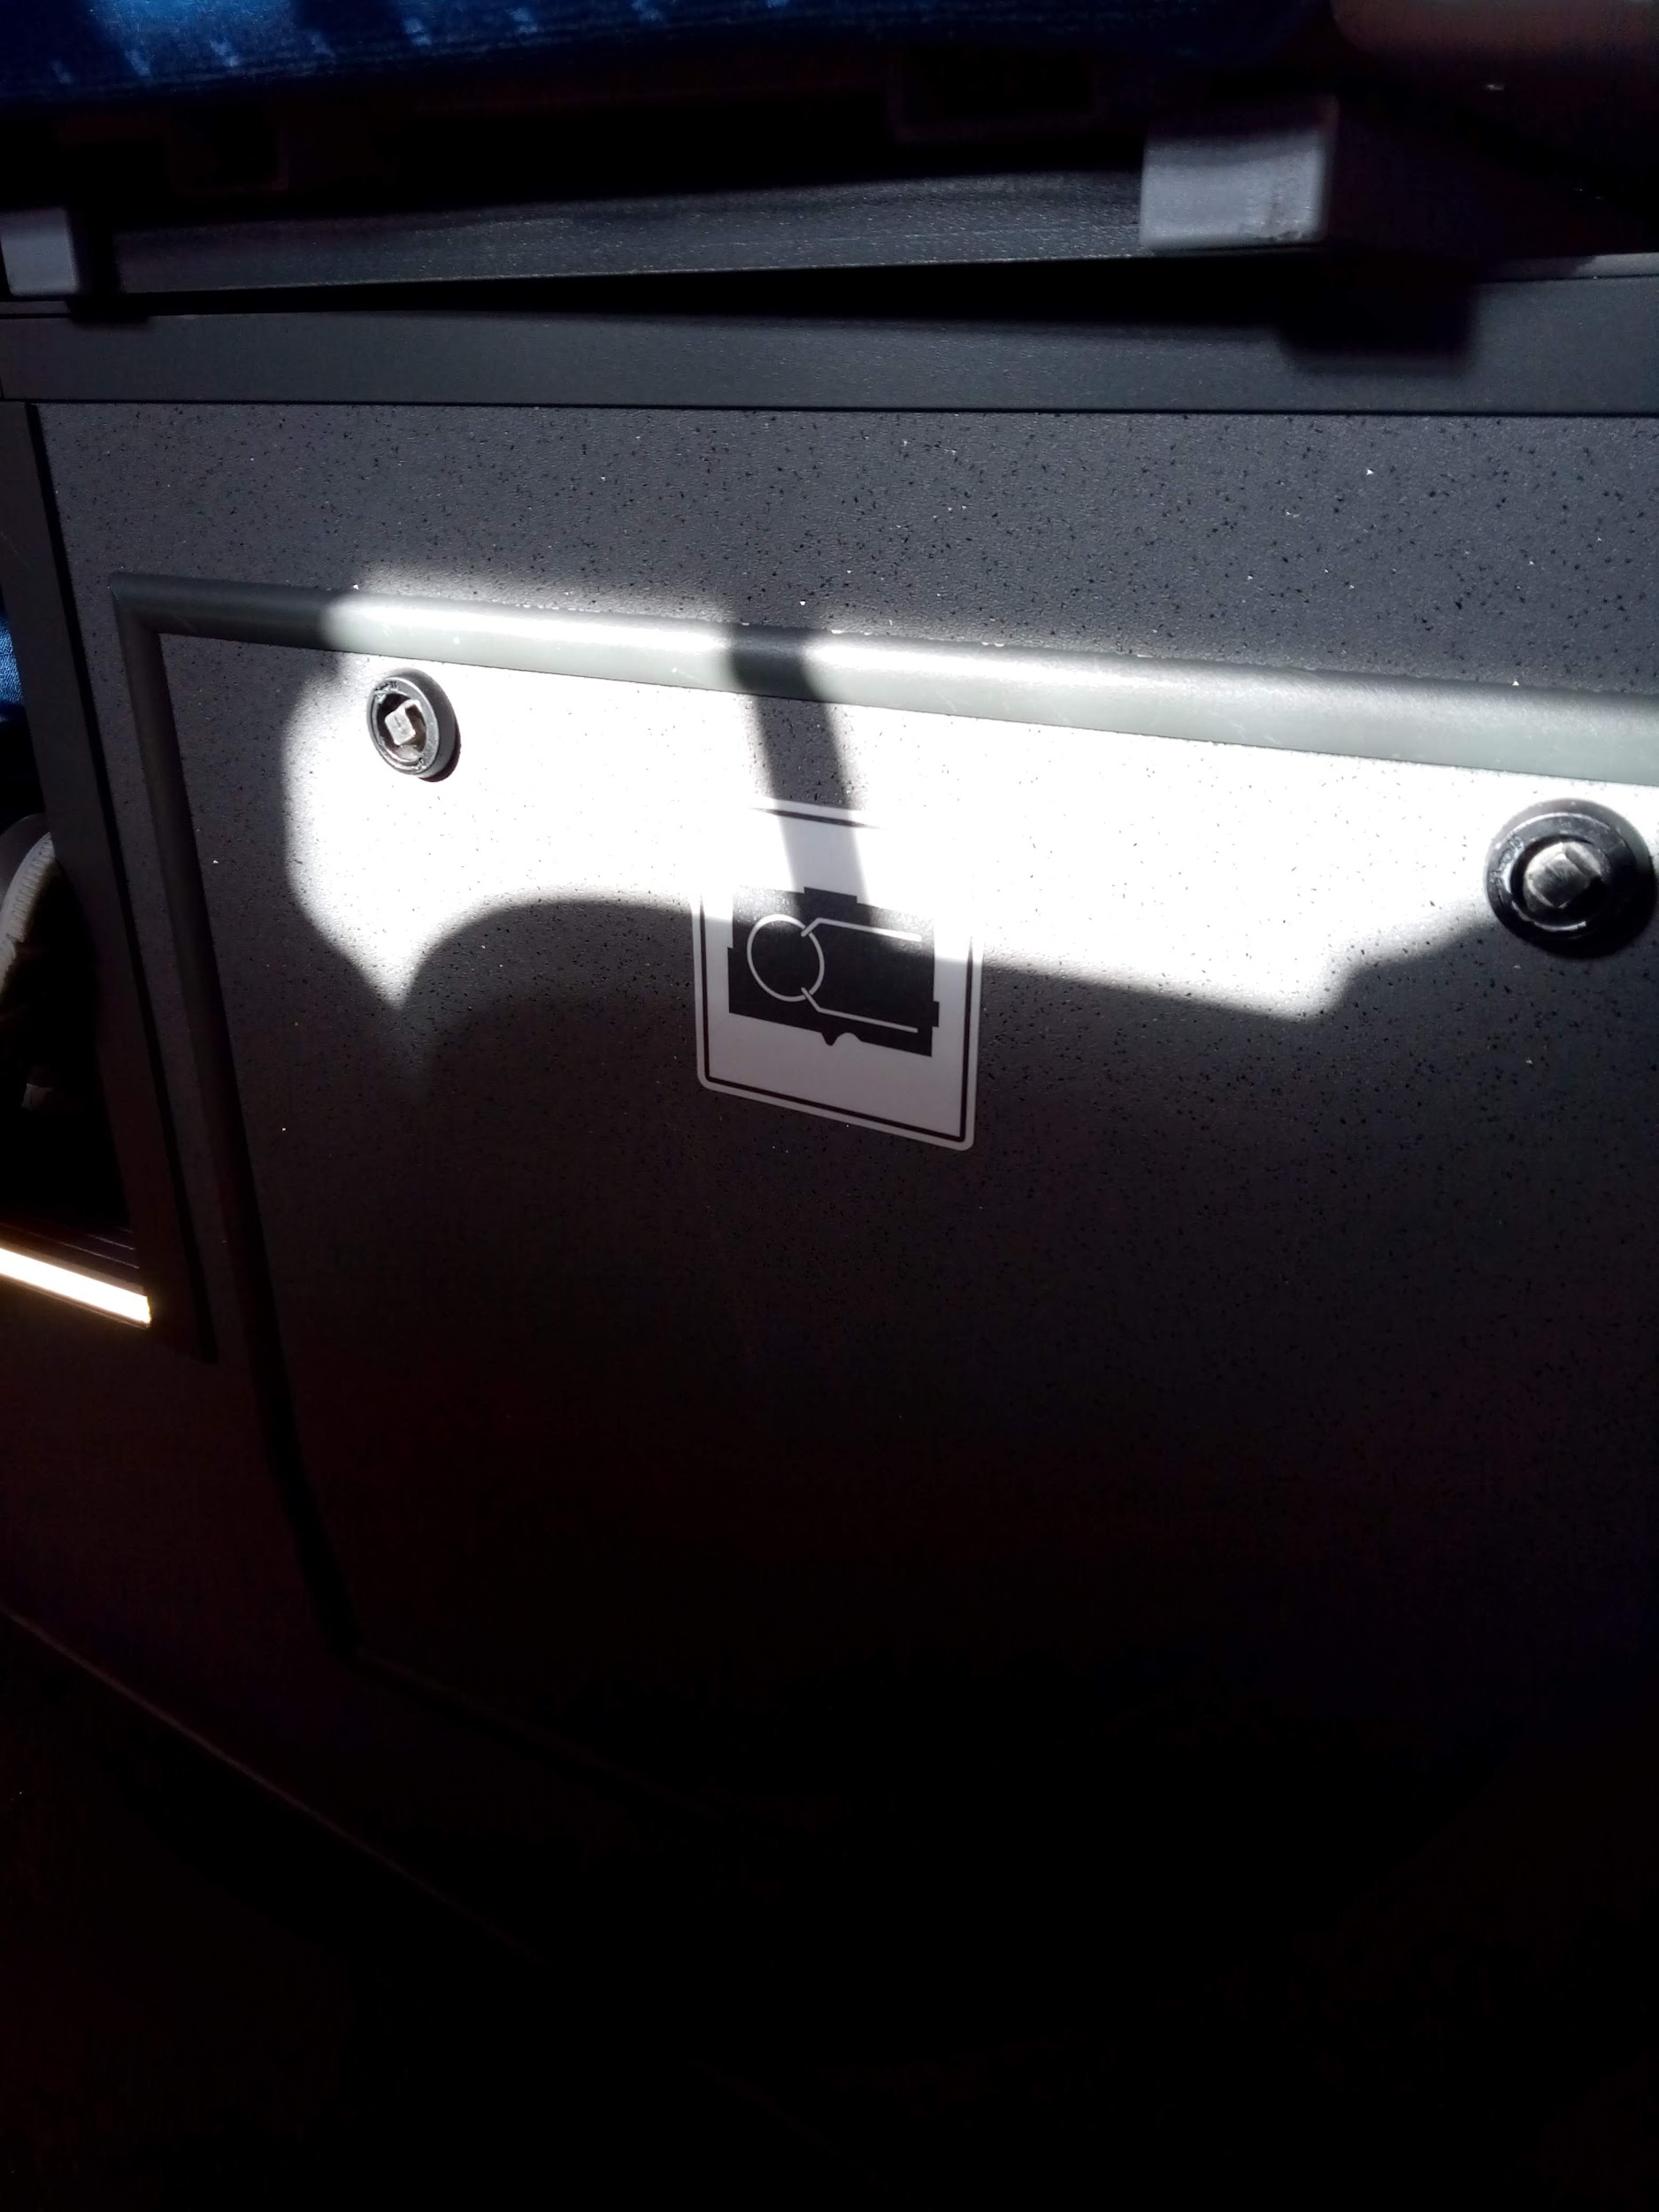
\includegraphics[width=6cm]{skryptkierownik-img/skryptkierownik-img047.jpg}}
\caption{Miejsce montażu wspornika, Wspornik sygnału Pc5, szfka pod fotelem}
\end{figure}

\section{Podsumowanie}
\begin{tcolorbox}[colback=black!5!white,colframe=green!75!black,width=18cm,title=Podsumowanie rozdziału]
	\begin{enumerate}
	\item Litera E namalowana na pojeździe oznacza:
	\begin{enumerate}
		\item Pojazd z przetwornicą statyczną,
		\item Pojazd z hamulcem elektrodynamicznym,
		\item Pojazd z hamulcem elektropneumatycznym.
	\end{enumerate}	
	\item Jakie zadanie w układzie hamulcowym wagonu spełnia zawór rozrządczy:
	\begin{enumerate}
		\item Uniemożliwia zablokowanie kół podczas hamowania,
		\item Steruje pracą układu hamulcowego wagonu,
		\item Reguluje ustawienie wstawek hamulcowych.
	\end{enumerate}
	\end{enumerate}
\end{tcolorbox}

\chapter{Wykonywanie szczegółowej i uproszczonej próby hamulca}

Próba hamulca ma na celu stwierdzenie sprawności hamulca zespolonego (pneumatycznego) pociągu. Należy sprawdzić ponadto działanie hamulca elektropneumatycznego. Jeśli pociąg kursuje na hamulcach ręcznych sprawdza się działanie tych hamulców. Potwierdzeniem przeprowadzenia próby hamulca jest karta prób hamulca. Drużynie trakcyjnej nie wolno uruchomić pociągu, jeśli nie dysponuje ona dokumentem potwierdzającym wykonanie, z pozytywnym wynikiem, wymaganej próby hamulca.
Karta próby hamulca po wykonaniu próby i wypełnieniu musi znajdować się w czynnej kabinie maszynisty.

W przypadku pociągu zestawionego z pojazdu kolejowego z napędem, składającego się z jednego lub wielu członów, wyposażonego w\textbf{ hamulce tarczowe}, posiadającego nierozłączalny w normalnej eksploatacji główny przewód hamulcowy oraz manometry lub wskaźniki wskazujące ciśnienie powietrza w cylindrach hamulcowych na wszystkich wózkach jezdnych i sygnalizację stanu zahamowania i odhamowania pojazdu kolejowego w kabinie sterowniczej, dopuszcza się jednoosobowe wykonywanie \textbf{uproszczonej} próby hamulca przez \textbf{maszynistę} na podstawie tych wskazań. W spółce Koleje Śląskie próbę taką obowiązkowo wykonuje maszynista.
\begin{marginfigure}
	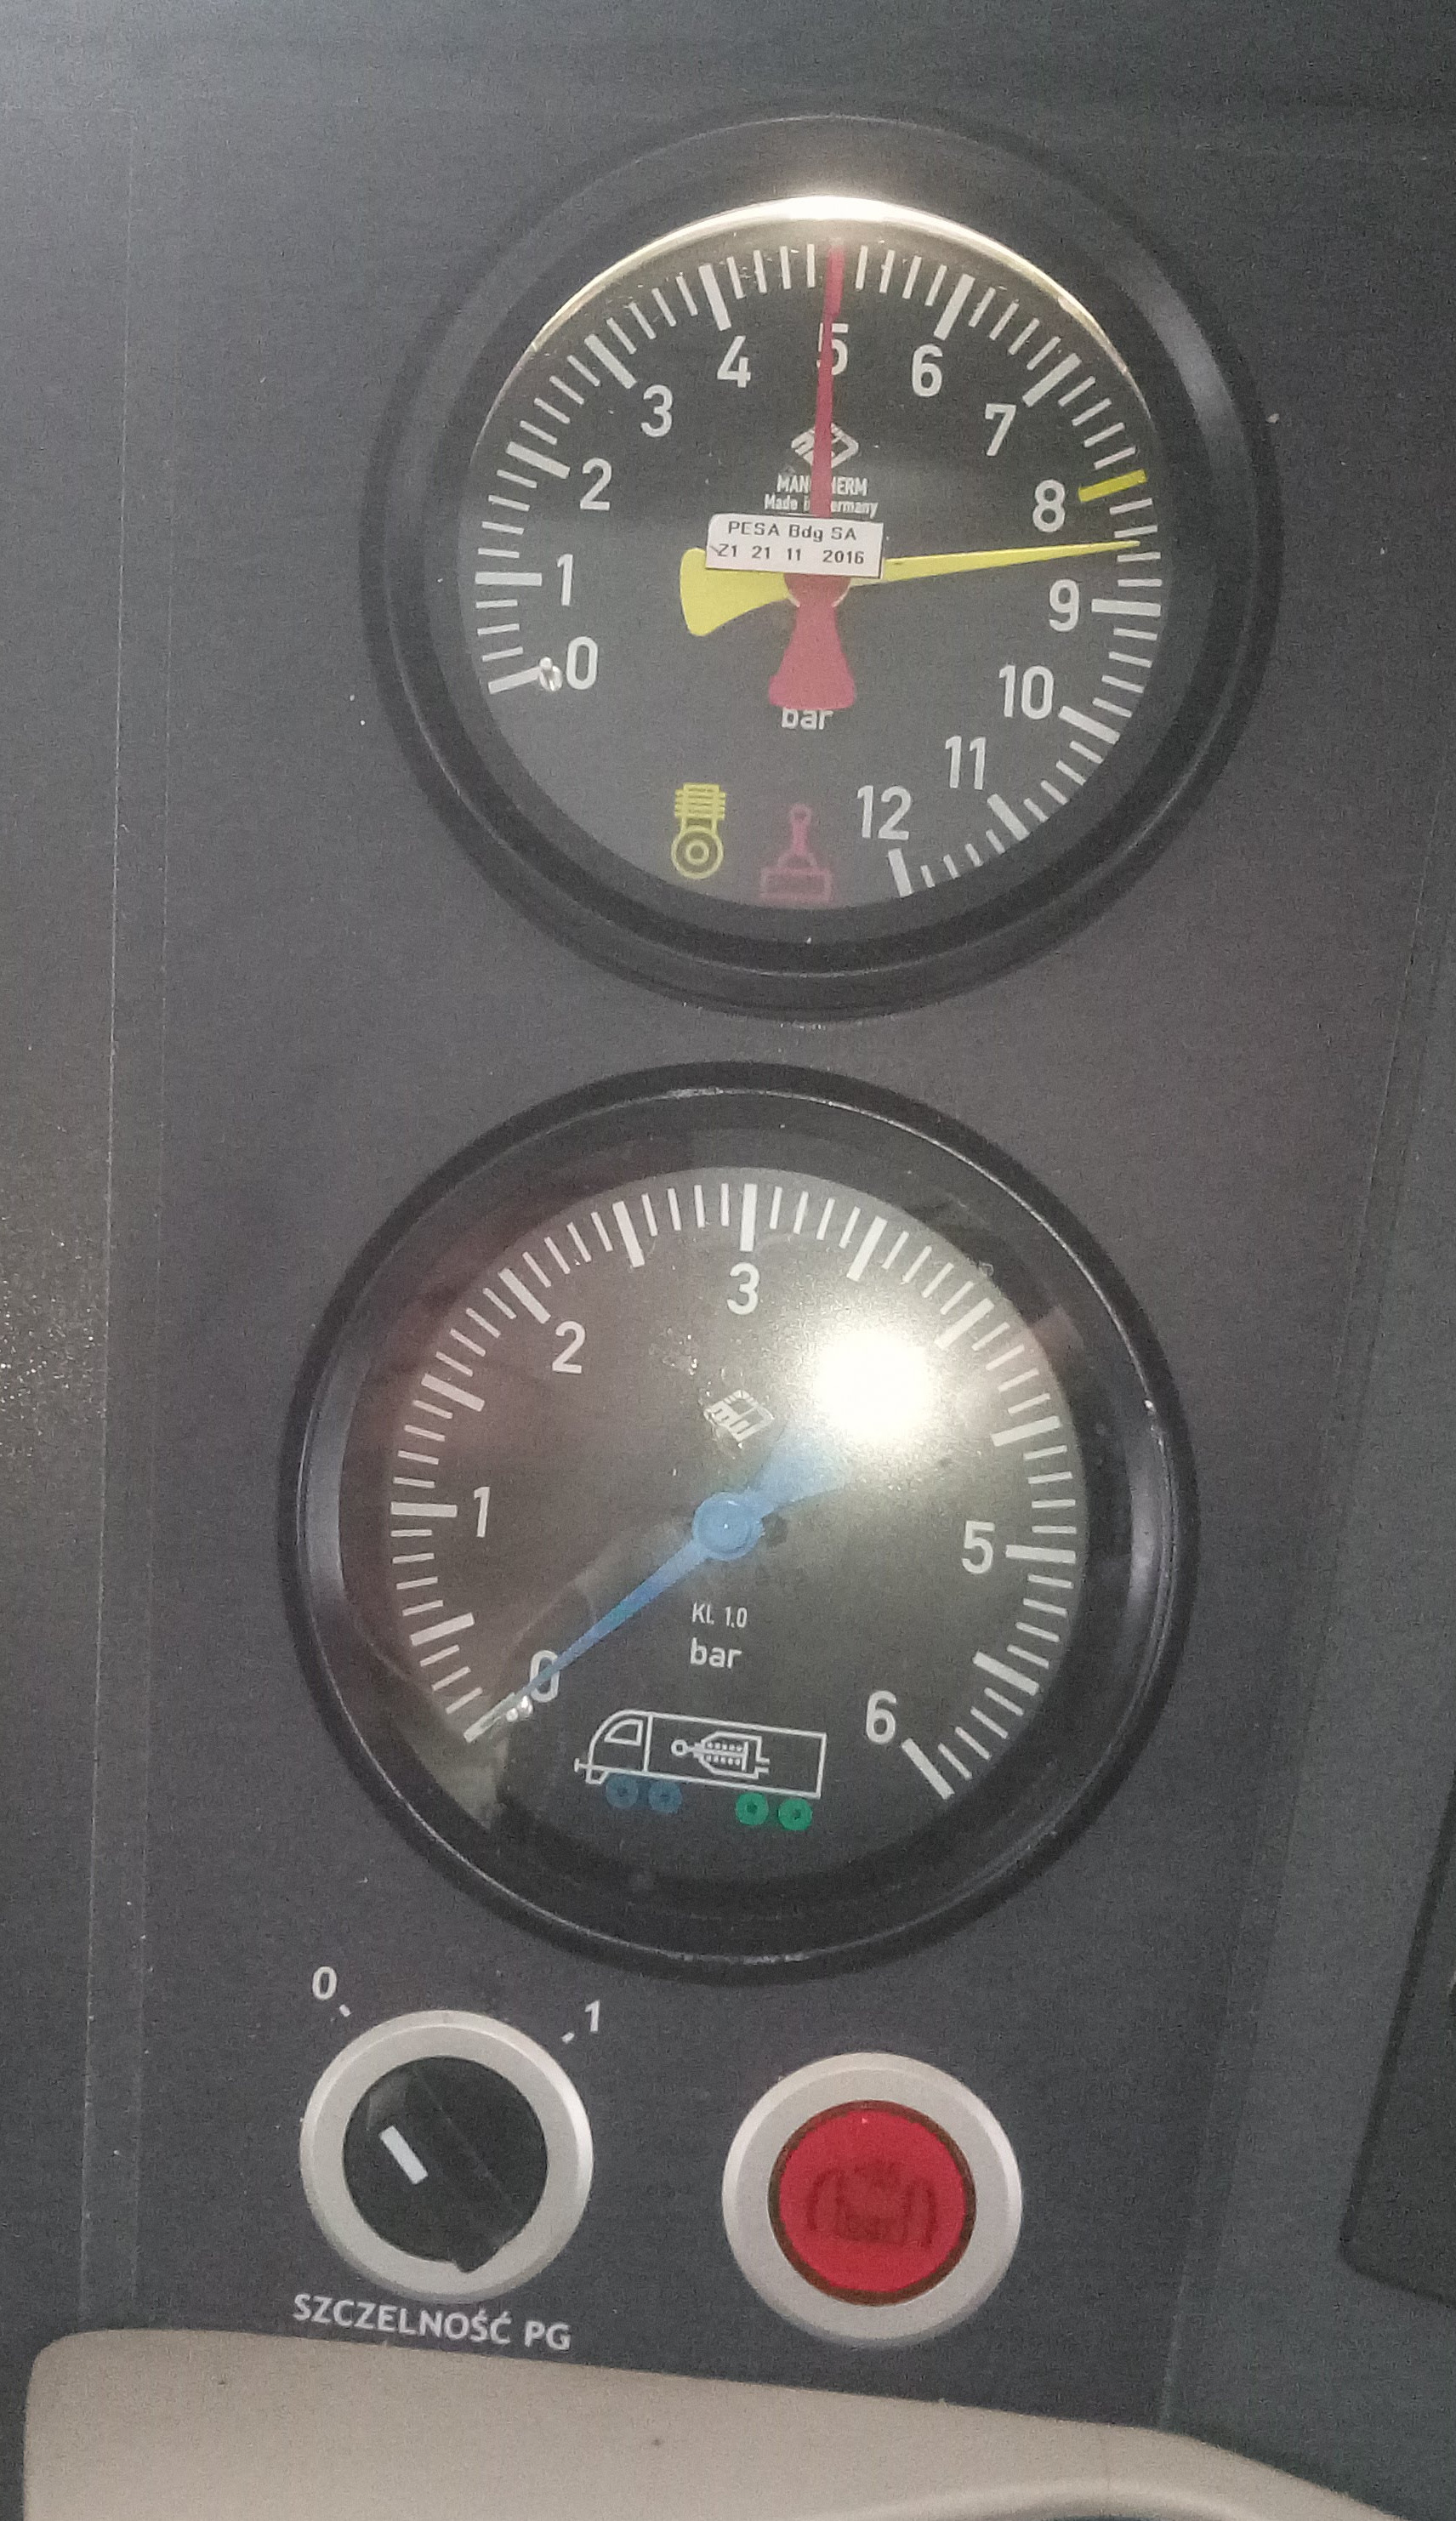
\includegraphics[width=5cm]{skryptkierownik-img/manometry-odhamowane.jpg}
	\caption{Manometry na pulpicie maszynisty EN76 w stanie odhamowanym. Wskazówka czerwona odnosi się do przewodu głównego, żółta do przewodu zasilającego}
\end{marginfigure}
\textbf{Szczegółową próbę hamulca} należy wykonać: 
\begin{itemize}
	\item przed wyprawieniem pociągu ze \textbf{stacji początkowej}; 
	
	\begin{itemize}
		\item odstępstwo od tej zasady może być stosowane dla pociągu, który po przybyciu na stację jest wyprawiony w dalszą
		drogę bez przeformowania lub bez naprawy urządzeń hamulcowych pod warunkiem, że przy tym składzie co najmniej jeden raz
		w ciągu poprzedzających \textbf{24 godzin} była wykonywana szczegółowa próba hamulca,\underline{ wtedy należy przeprowadzić \textbf{uproszczoną próbę hamulca}}; 
	\end{itemize}
	\item na stacjach wyznaczonych w rozkładzie jazdy pociągów;
	\item gdy urządzenia hamulcowe w składzie pociągowym lub w pociągu \textbf{nie były} \textbf{zasilane} sprężonym powietrzem \textbf{dłużej niż 12 godzin}; 
	\item po zmianie składu pociągu, jeżeli doczepione pojazdy kolejowe stanowią \textbf{więcej niż 50 \% masy brutto składu pociągu}; nie jest wymagana szczegółowa próba hamulca, pod warunkiem, że włączane pojazdy kolejowe znajdowały się w pociągach, w których co najmniej jeden raz w ciągu poprzedzających 24 godzin była wykonywana szczegółowa próba hamulca;
	
	\item jeżeli podczas uproszczonej próby hamulców stwierdzono, że hamulec jednego z dwóch ostatnich dwóch wagonów lub innych pojazdów kolejowych \textbf{nie hamuje lub nie odhamowuje}; 
	\item jeżeli maszynista stwierdzi nie działanie lub nie jest pewny prawidłowego działania hamulców (na każde żądanie maszynisty); 
	\item po przeładowaniu głównego przewodu hamulcowego pociągu powyżej \textbf{0,55MPa} i opróżnieniu komór i zbiorników sterujących za pomocą odluźniaczy.
\end{itemize}

\underline{Próba szczegółowa hamulca zespolonego pociągu polega na}: 
\begin{marginfigure}
	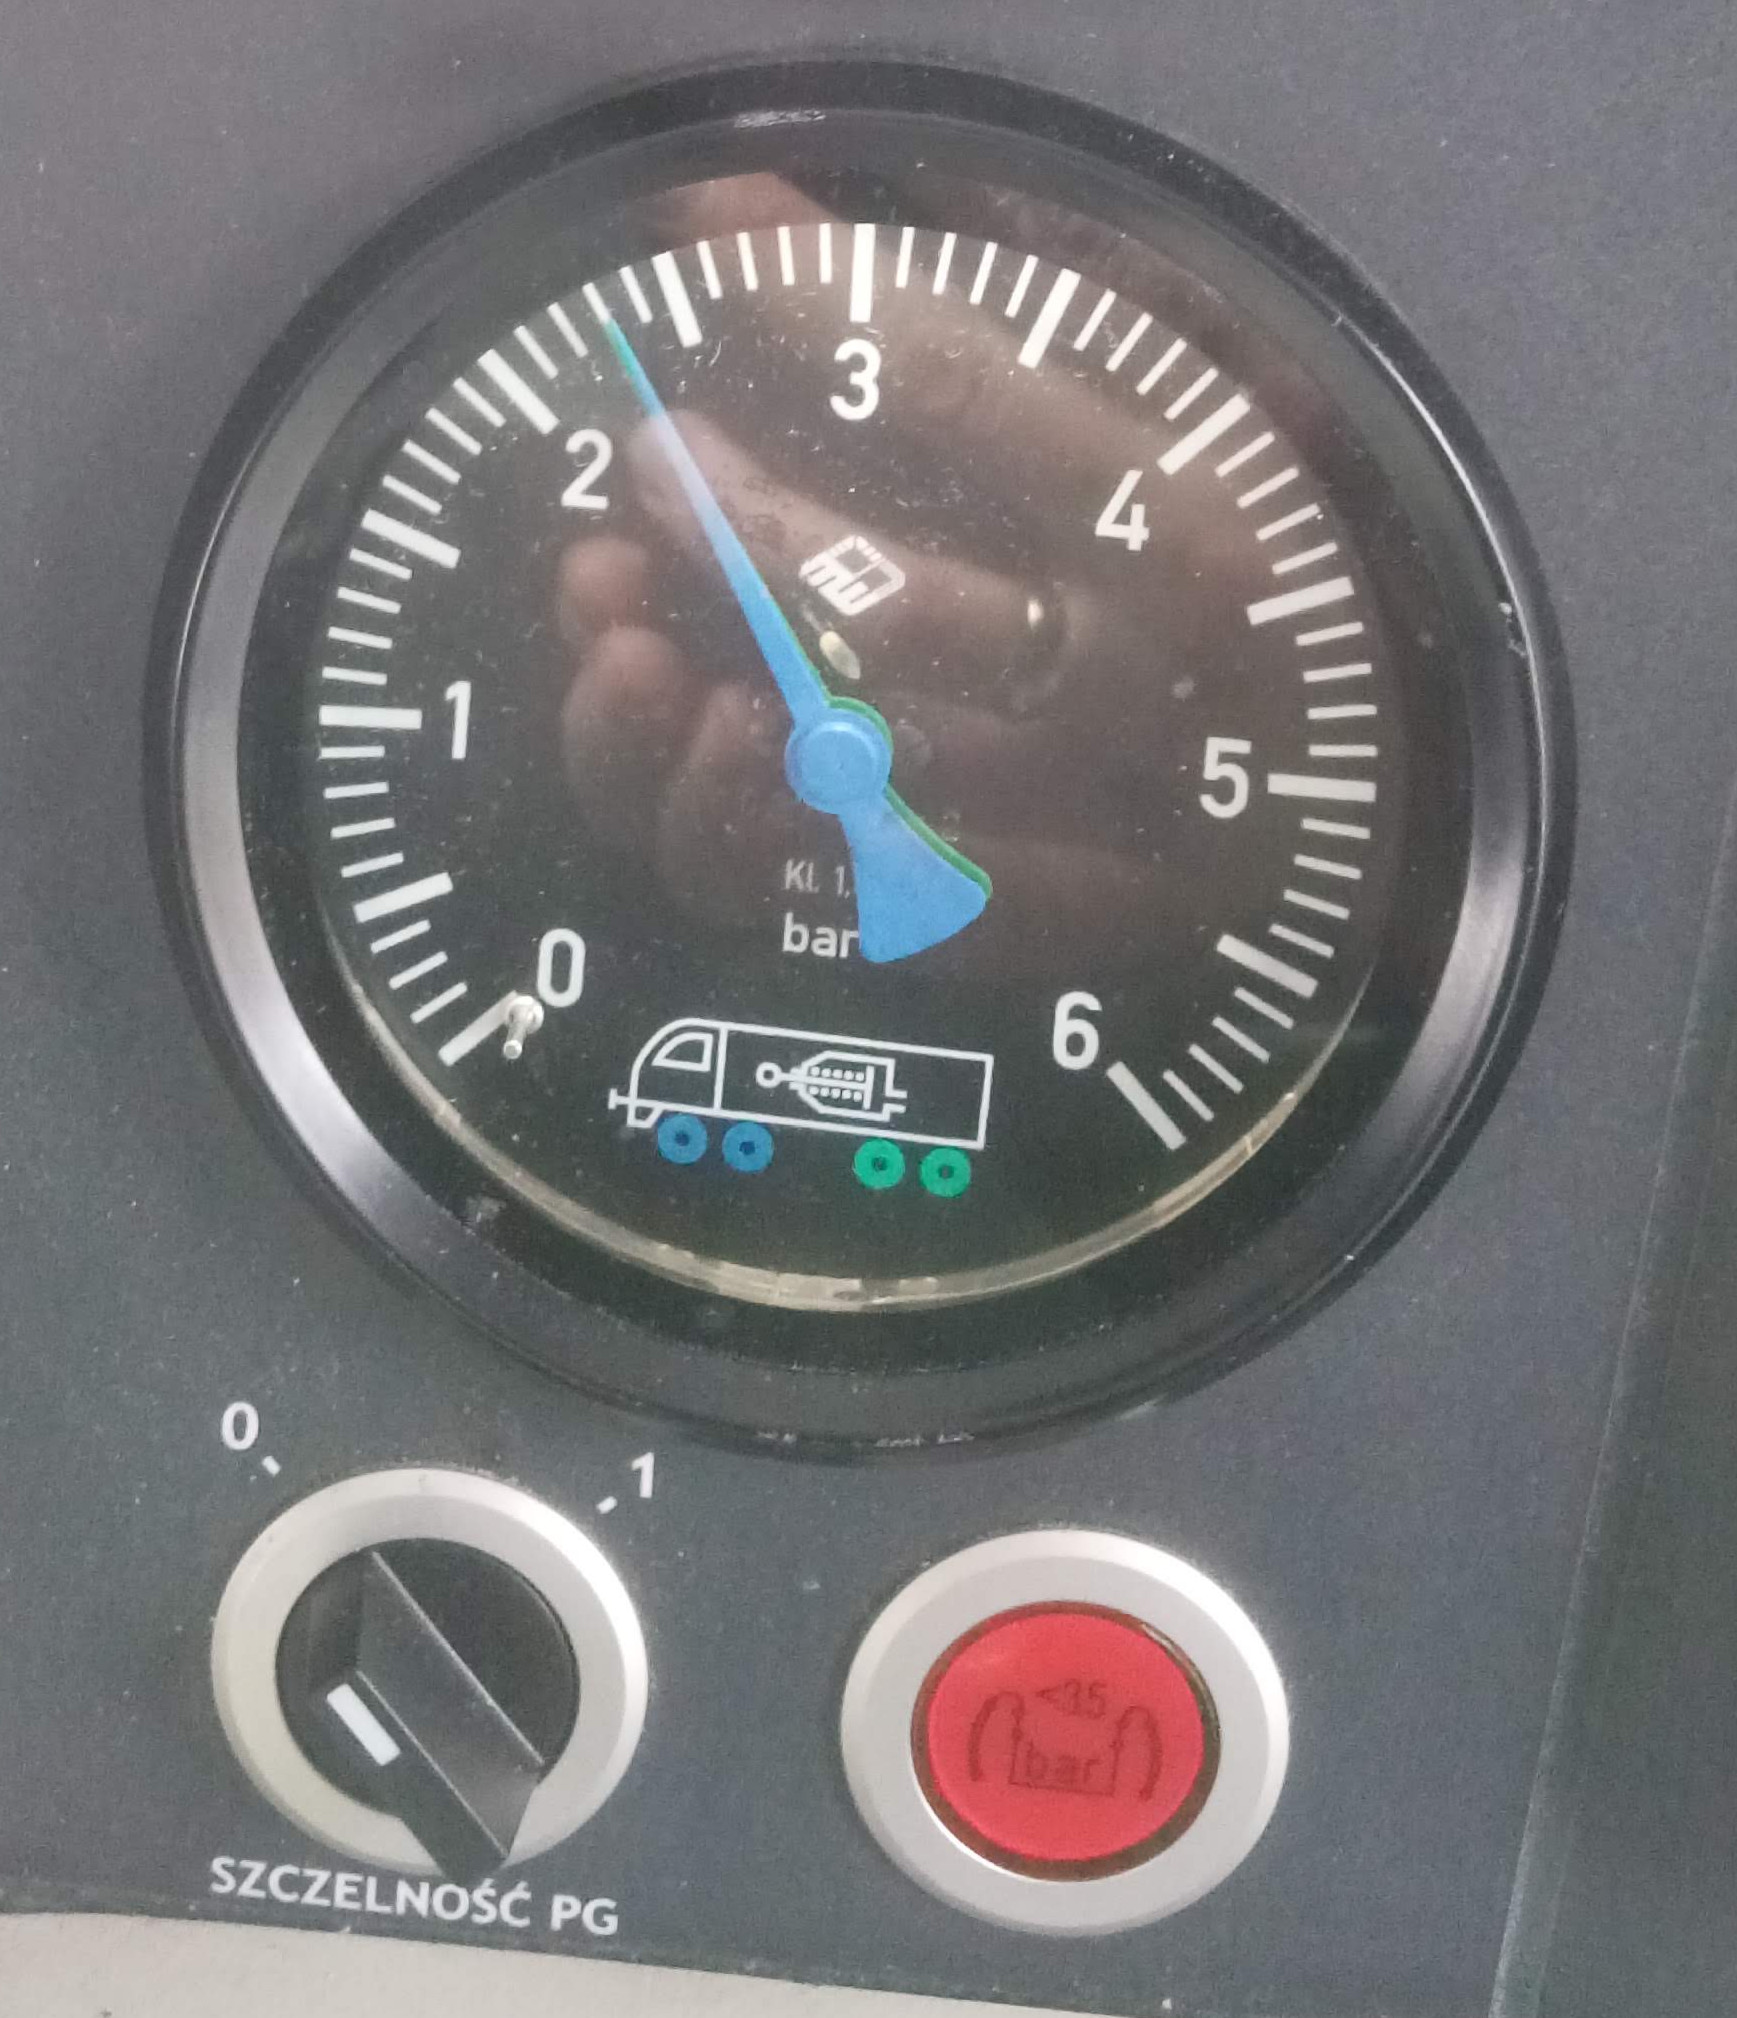
\includegraphics[width=5cm]{skryptkierownik-img/manometry-zahamowane-ep.jpg}
	\caption{Manometry cylindra hamulcowego w EN76 w czasie hamowania}
\end{marginfigure}
\begin{itemize}
	\item upewnieniu się że skład jest zabezpieczony przed zbiegnięciem, a hamulec \textbf{ręczny} odhamowany.
	\item skontrolowaniu we wszystkich pojazdach włączonych do składu pociągu połączeń sprzęgów i nastawień hamulca oraz sprawdzeniu na końcu pociągu czy w przewodzie głównym znajduje się sprężone powietrze i pomiarze ciśnienia tego powietrza (w EZT pomiar ciśnienia na manometrach w tylnej kabinie), 
	\item sprawdzeniu szczelności układu pneumatycznego hamulca w stanie zahamowanym (na manometrach w tylnej kabinie, spadek o mniej niż 0,05MPa w ciągu 5 minut), 
	\begin{figure*}
	\subfloat{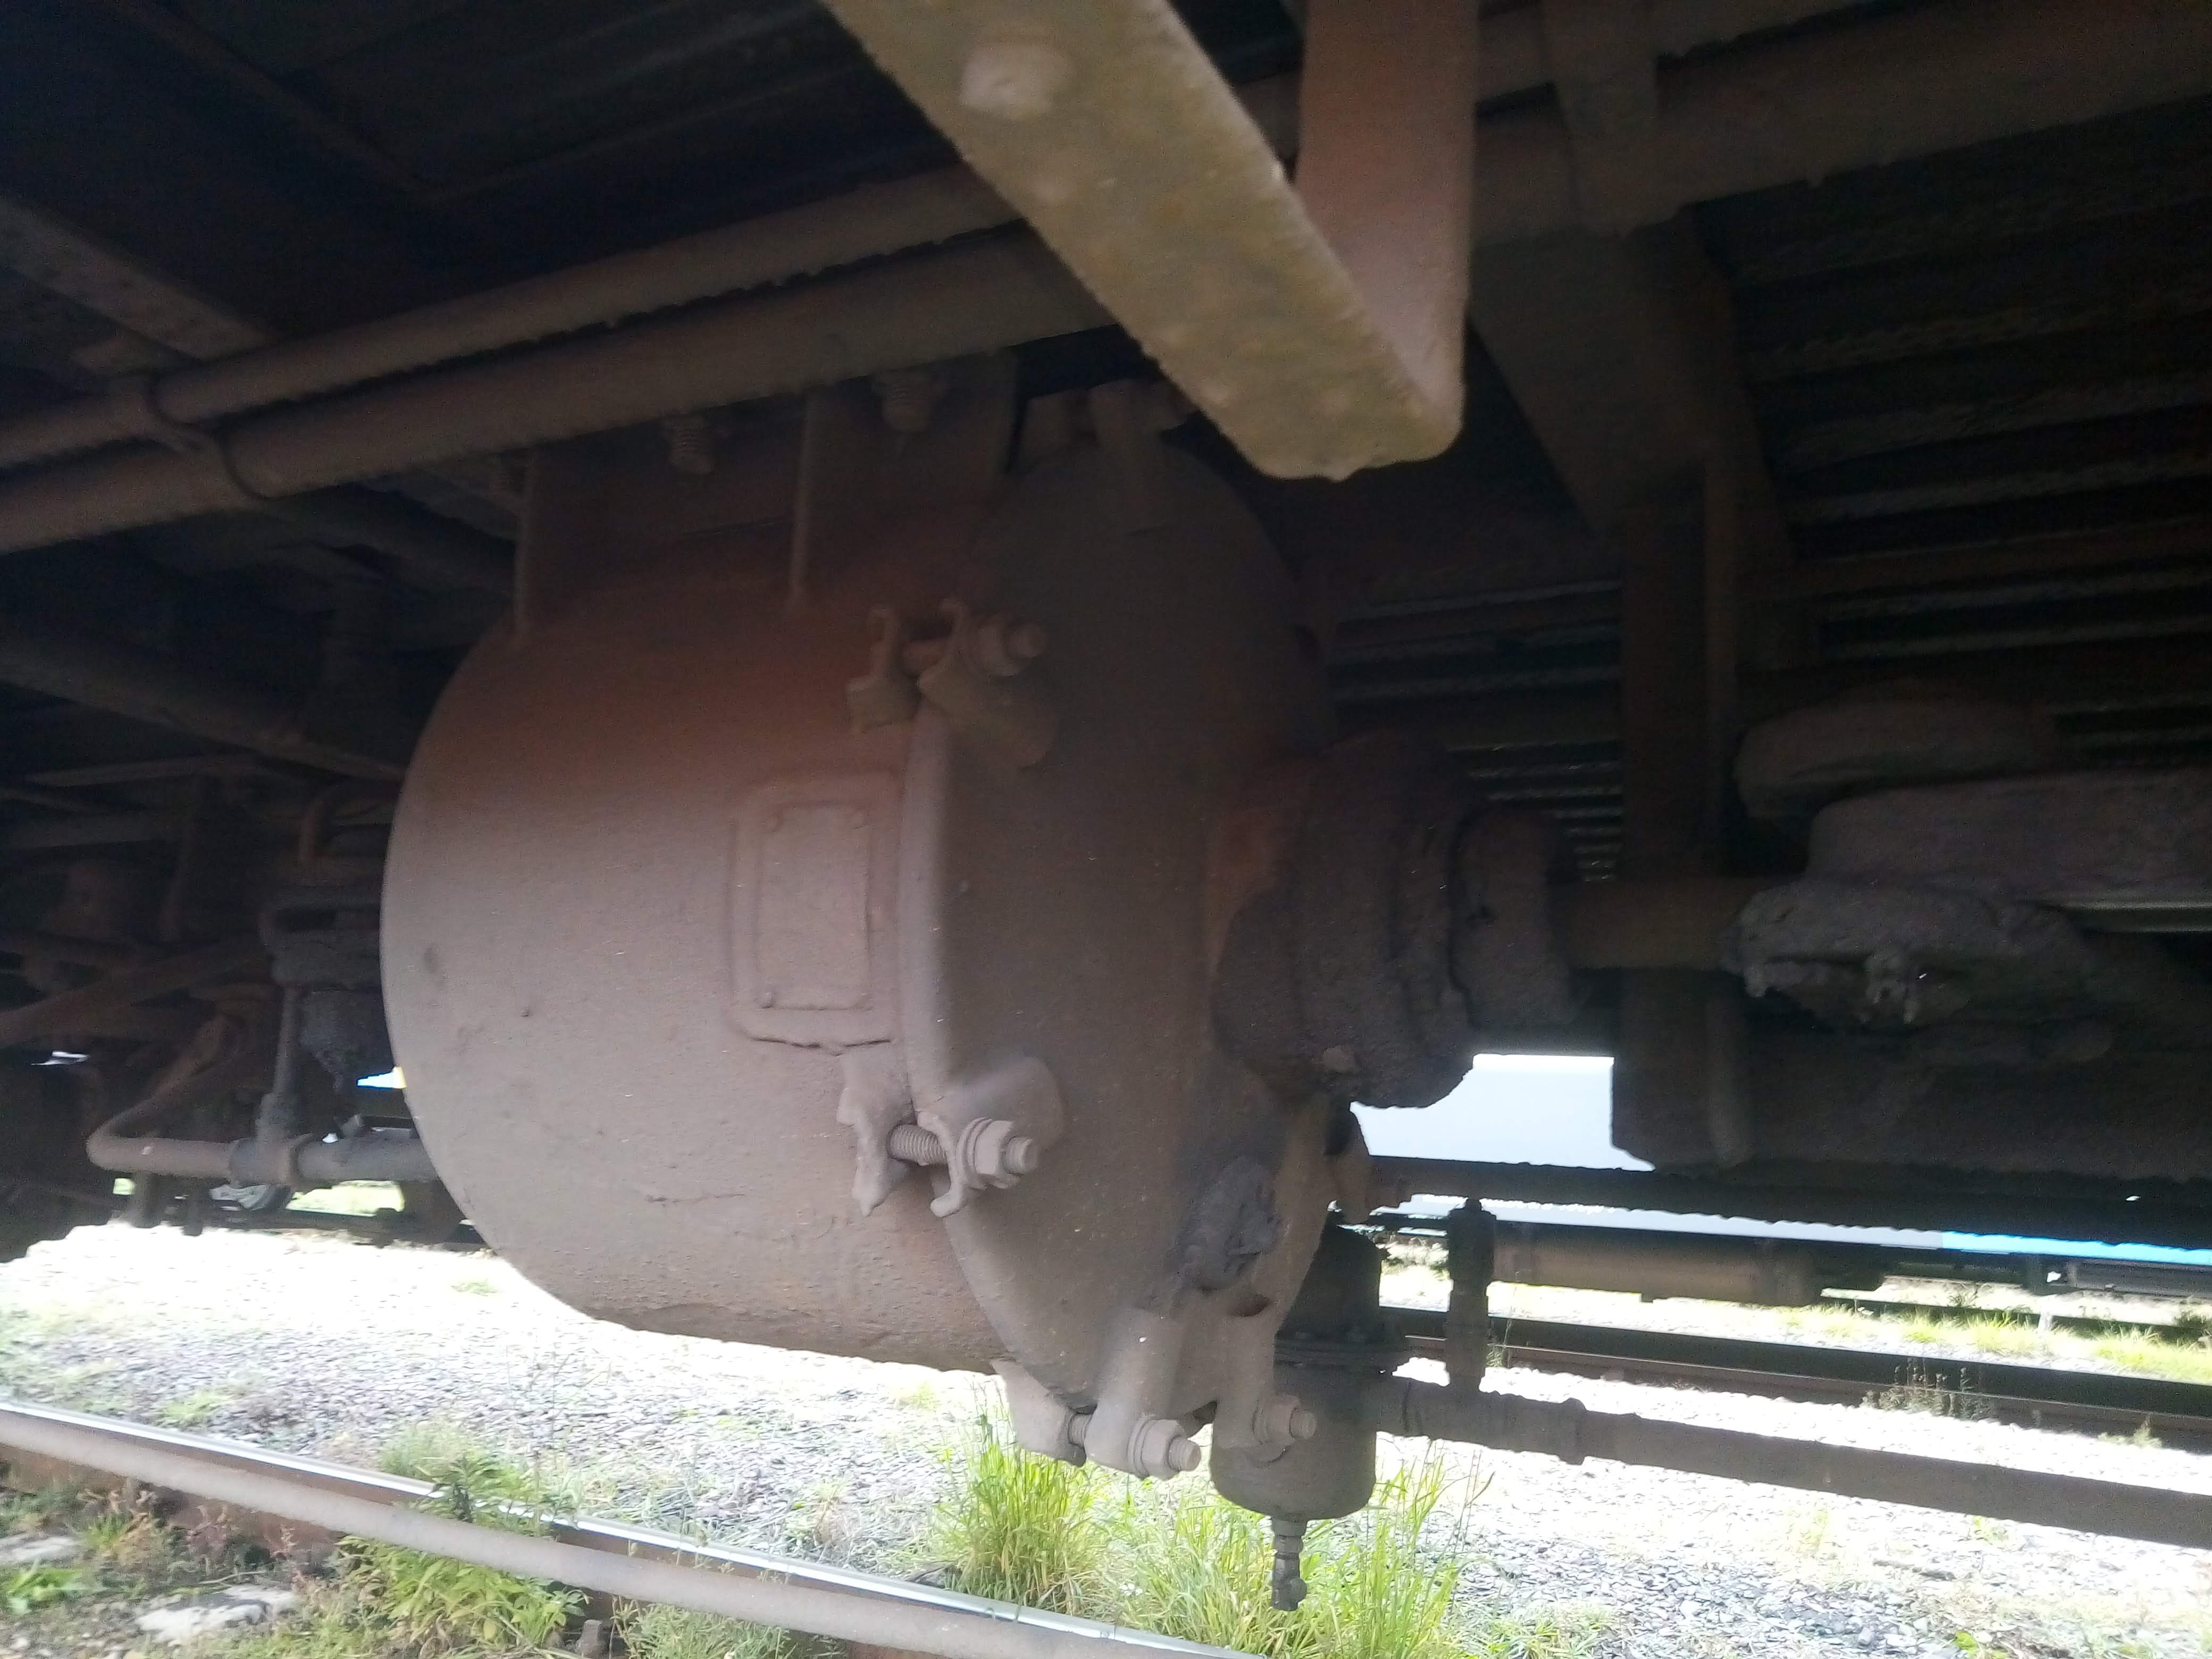
\includegraphics[width=7cm]{skryptkierownik-img/skryptkierownik-img033.jpg}}
	\subfloat{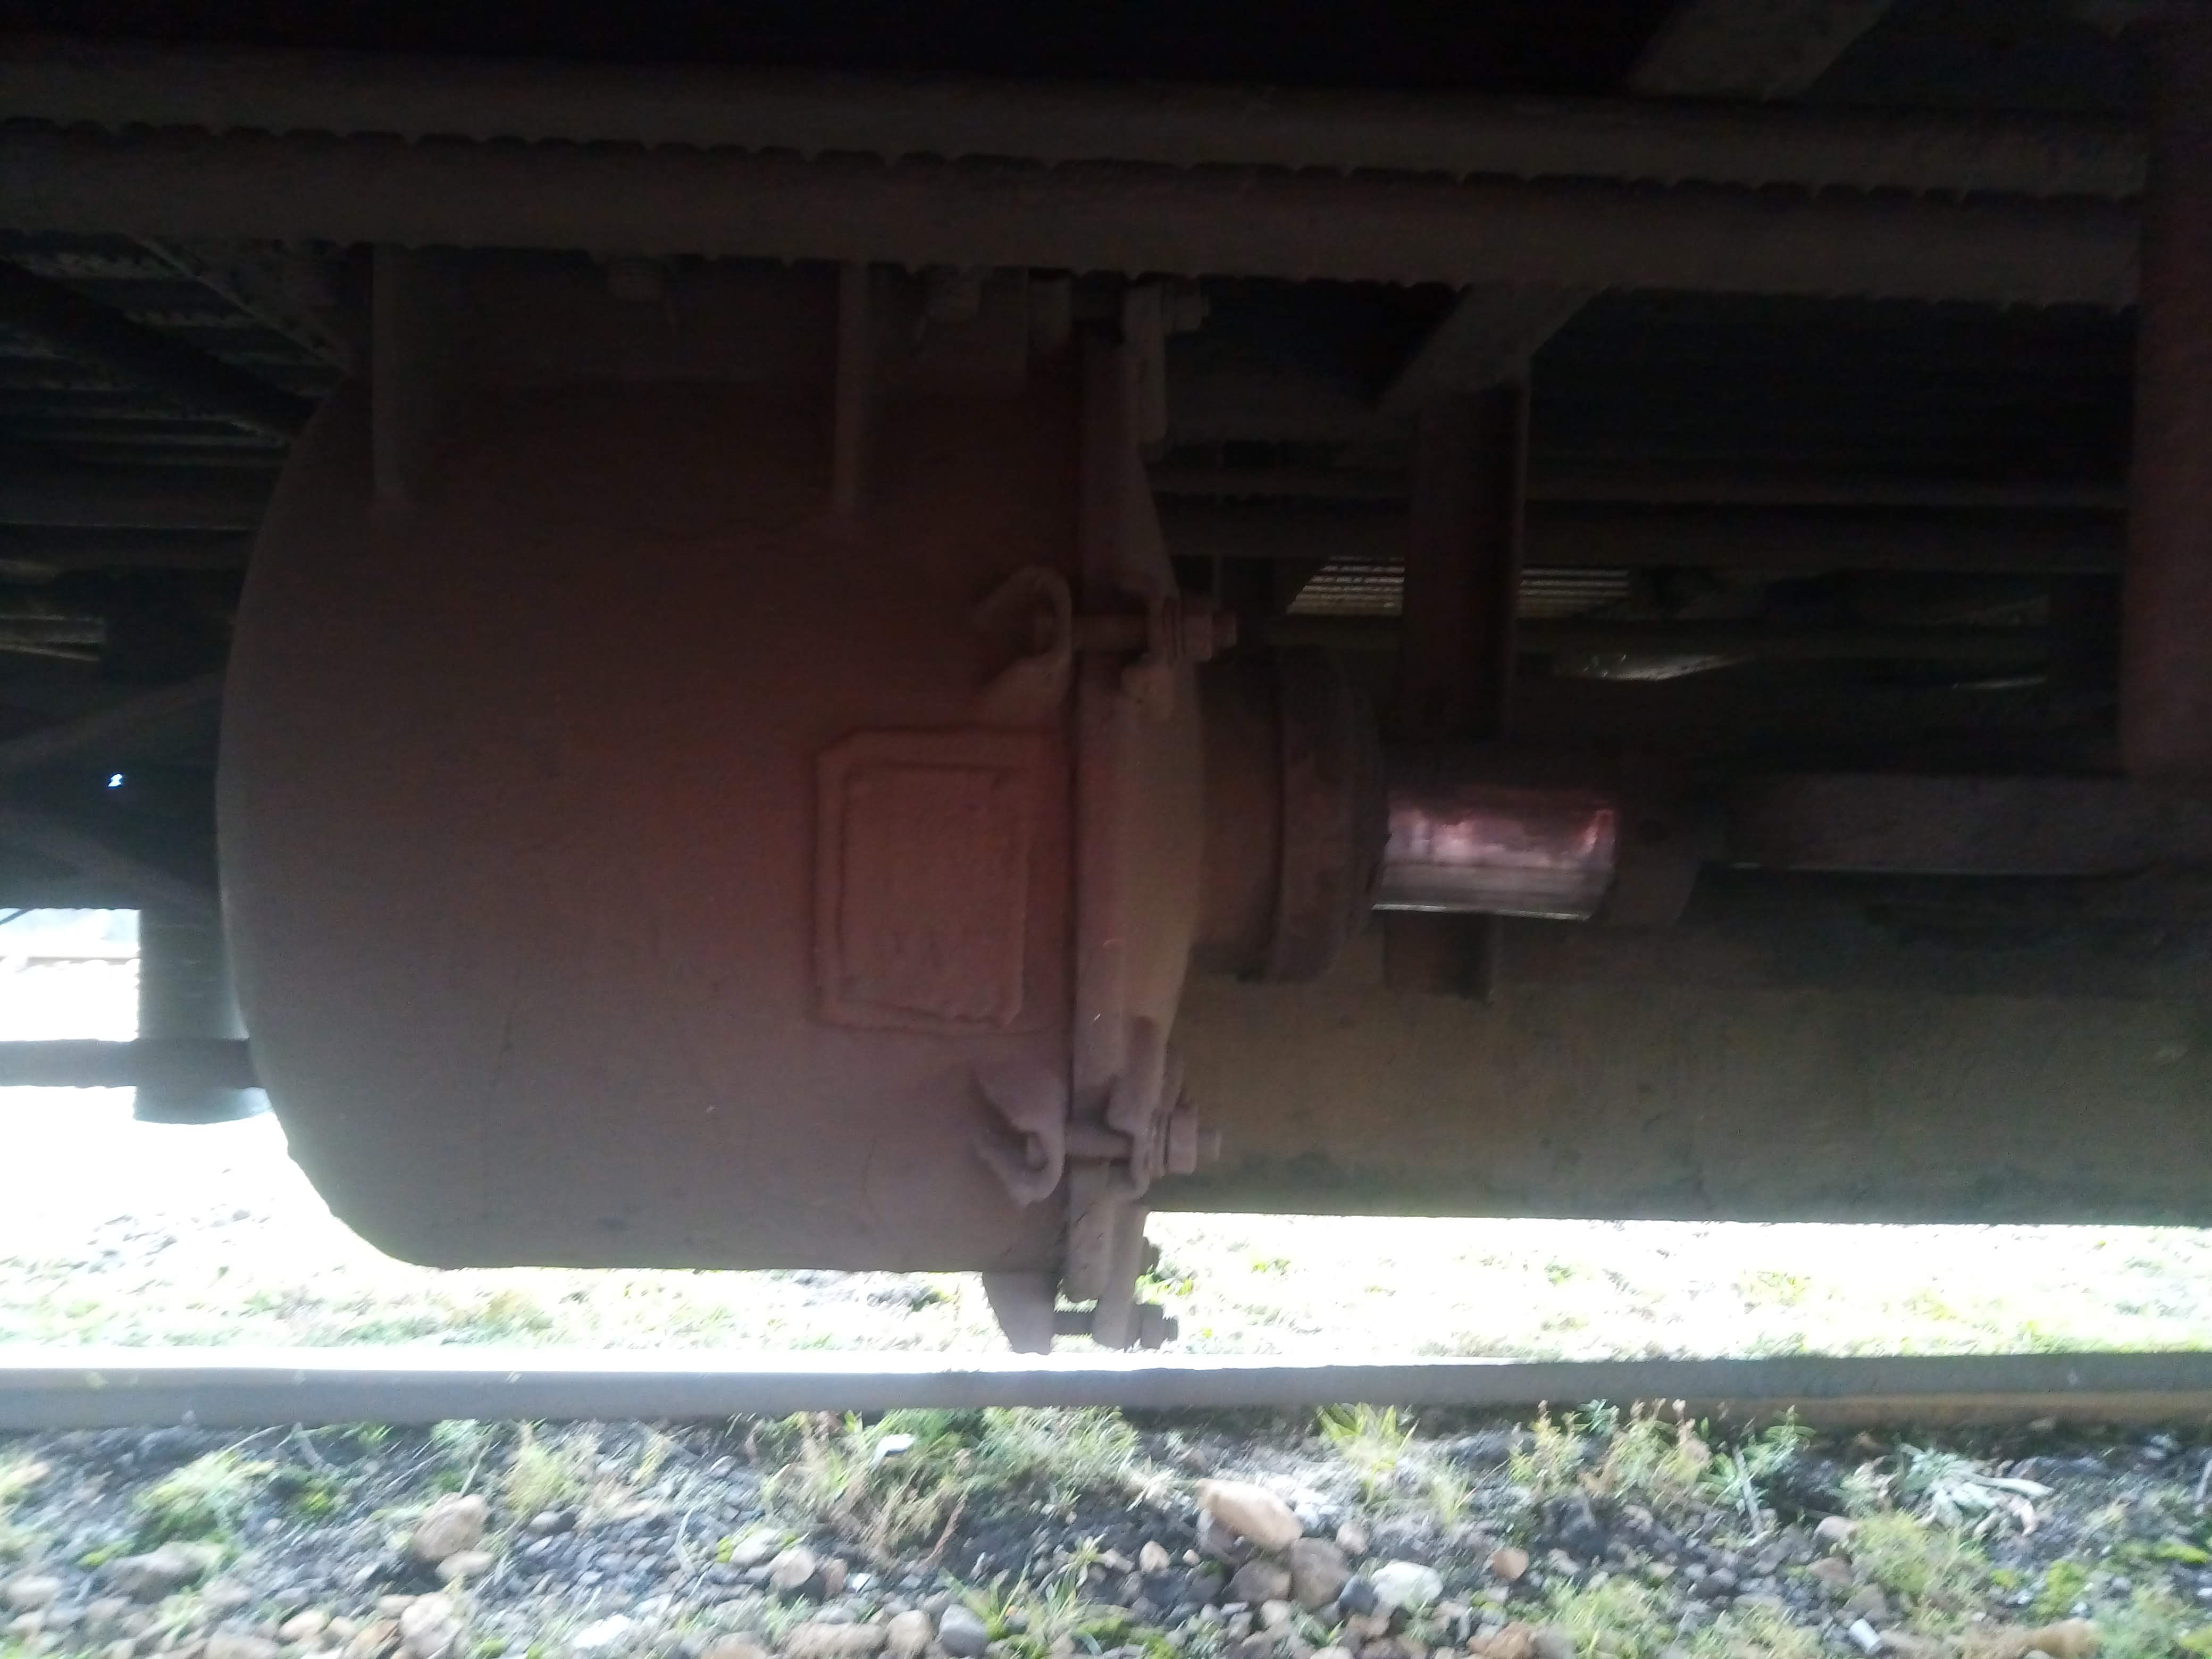
\includegraphics[width=7cm]{skryptkierownik-img/skryptkierownik-img034.jpg}}
	\caption{Cylinder hamulcowy w stanie odhamowanym/zahamowanym}
\end{figure*}

	\item sprawdzeniu, czy w składzie pociągu hamują wszystkie wagony z czynnym hamulcem zespolonym, (sprawdzenie czy wstawki hamulcowe zostały dociśnięte do kół, oraz czy tłoki cylindrów hamulcowych wysunęły się (ok. 14cm), a jeśli wagony te mają hamulec tarczowy - czy wskaźniki pokazują zahamowanie), 
	
	\item sprawdzeniu, czy w składzie pociągu luzują hamulce wszystkich pojazdów z czynnym hamulcem zespolonym, (sprawdzenie czy wstawki hamulcowe odsunęły się od kół, oraz tłoki cylindrów hamulcowych wsunęły się w całości do cylindra, a jeśli wagony te mają hamulec tarczowy - czy wskaźniki pokazują odhamowanie)
	\marginnote{Ciiiilinder ;$)$ }
	\item należy wykonać ponownie procedurę dla hamowania hamulcem elektropneumatycznym.
	\item sprawdzeniu, czy pod względem rozmieszczenia pojazdów z czynnym hamulcem zespolonym skład pociągu jest prawidłowo zestawiony.

Próbę szczegółową wykonujemy z tej kabiny, z której będzie prowadzony pierwszy pociąg.	
\end{itemize}
\textbf{Uproszczoną próbę hamulców} należy wykonać w pociągu, w którym po dokonaniu próby szczegółowej:
\begin{itemize}
	\item nastąpiło zamknięcie lub otwarcie, nawet częściowe lub chwilowe, \textbf{przewodu głównego hamulca}, w którymkolwiek miejscu pociągu, z wyjątkiem zaworu maszynisty w czynnej kabinie sterującej i innych urządzeń na pojeździe trakcyjnym powodujących samoczynne hamowanie; w przypadku dołączenia pojazdów kolejowych do pociągu wykonuje się próbę uproszczoną hamulców pociągu, a pojazdy kolejowe dołączone poddaje się takim badaniom, jak podczas próby szczegółowej hamulca; badania te nie są wymagane w przypadku dołączenia pojazdów kolejowych na początku lub końcu pociągu i gdy włączane pojazdy kolejowe były używane w pociągach, w których co najmniej jeden raz w ciągu poprzedzających 24 godzin była wykonywana szczegółowa próba hamulca, a okres braku zasilania sprężonym powietrzem hamulców tych wagonów lub innych pojazdów kolejowych nie przekracza 12 godzin; 
	\item \textbf{wyłączono co najmniej jeden pojazd} kolejowy ze składu pociągu, 
	\item nastąpiła \textbf{zmiana przedziału} sterowniczego; 
	\item \textbf{wyłączenie zasilania sprężonym powietrzem} urządzeń hamulcowych w pociągu trwało do \textbf{12 godzin}; 
	\item szczegółowa próba hamulców była wykonana przy użyciu sieci stałej sprężonego powietrza lub innego pojazdu trakcyjnego, nieprzeznaczonego do prowadzenia tego pociągu; 
	\item nastąpiło zamknięcie lub otwarcie, nawet częściowe lub chwilowe, \textbf{przewodu zasilającego}, w którymkolwiek miejscu pociągu, którego hamulce są nastawione na przebieg hamowania \textbf{„R + Mg"};
\end{itemize}



\underline{Uproszczoną próbę hamulca wykonuje się w sposób następujący:} 
\begin{itemize}
	\item pracownik znajdujący się za ostatnim pojazdem pociągu: stwierdza, przez kilkukrotne otwieranie i zamykanie kurka końcowego przewodu głównego na końcu pociągu, że w przewodzie głównym znajduje się sprężone powietrze, a jeżeli jest to niemożliwe, sprawdza wskazanie manometru w tylnej kabinie maszynisty: 
	\begin{itemize}
		\item zamyka kurek, 
		\item upewnia się, że ostatni pojazd jest w stanie odhamowanym, 
		\item podaje do czoła pociągu sygnał Rh1 "Zahamować", 
	\end{itemize}
\begin{marginfigure}
	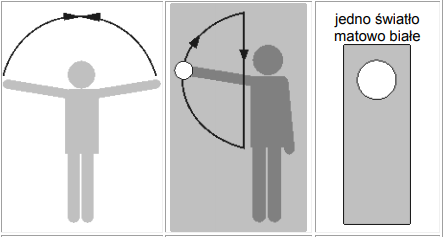
\includegraphics[width=6cm]{skryptkierownik-img/skryptkierownik-img069.png}
	\caption{Rh1 i Rhs1 Zahamować}
\end{marginfigure}
	\item maszynista po odebraniu sygnału Rh1 "Zahamować" wykonuje hamowanie służbowe, 
	\item pracownik dokonujący próby hamulca sprawdza czy wstawki hamulcowe \textbf{dwóch ostatnich pojazdów} są dociśnięte do kół, oraz czy tłoki cylindrów hamulcowych wysunęły się, a jeśli wagony te mają hamulec tarczowy - czy wskaźniki pokazują stan zahamowania, 
	\item po stwierdzeniu, że w sprawdzanych wagonach hamulec zahamował prawidłowo, pracownik wykonujący próbę podaje do czoła pociągu sygnał Rh2 "Odhamować",
\begin{marginfigure}
	\includegraphics[width=6cm]{skryptkierownik-img/skryptkierownik-img067.png}
	\caption{Rh2 i Rhs2 Odhamować}
\end{marginfigure}

	\item dokonujący próby sprawdza czy wstawki hamulcowe ostatnich dwóch pojazdów odsunęły się od kół, oraz czy tłoki cylindrów hamulcowych wsunęły się, a jeśli wagony te mają hamulec tarczowy - czy wskaźniki pokazują odhamowanie; 
	\item należy wykonać ponownie procedurę dla hamowania hamulcem elektropneumatycznym.
	\item jeśli hamulce dwóch ostatnich wagonów zahamowują i odhamowują poprawnie, to dokonujący próbę podaje do czoła pociągu sygnał Rh3 "Hamulce działają poprawnie".
	
\begin{marginfigure}
		\includegraphics[width=6cm]{skryptkierownik-img/skryptkierownik-img068.png}
		\caption{Rh3 i Rhs3 Hamulce działają poprawnie}
\end{marginfigure}

\end{itemize}

\section{Sygnały podawane przy próbie hamulca}

W celu nawiązania łączności między pracownikami wykonującymi próbę hamulca zespolonego pociągu i zapewnienia właściwej organizacji przeprowadzenia prób, stosuje się sygnały:

Rh1 i Rhs1 Zahamować
Rh2 i Rhs2 Odhamować
Rh3 i Rhs3 Hamulce działają poprawnie

W przypadku złej widoczności spowodowanej warunkami atmosferycznymi lub innymi (np. łuk toru), przy dokonywaniu prób hamulców w miejscach realizowanych budów, stacjach nie posiadających stałych urządzeń sygnalizacyjnych obsługa pociągu, powinna współdziałać w przekazywaniu sygnałów ręcznych. Dopuszcza się możliwość potwierdzania podawanych sygnałów przez radiotelefon przenośny i przewoźny, podczas dokonywania próby hamulca poza komendami przekazywanymi przez radiotelefon, powinno się sygnały przekazywać ręcznie.

\begin{tcolorbox}[colback=black!5!white,colframe=white!55!black,title=Pytania testowe]
	\begin{enumerate}
		\item Szczegółową próbę hamulca należy wykonać:
		\begin{enumerate}
			\item Gdy urządzenia hamulcowe w składzie pociągowym lub w pociągu nie były zasilane sprężonym powietrzem dłużej niż 12 godzin,
			\item Gdy urządzenia hamulcowe w składzie pociągowym lub w pociągu nie były zasilane sprężonym powietrzem krócej niż 12 godzin,
			\item Gdy urządzenia hamulcowe w składzie pociągowym lub w pociągu nie były zasilane sprężonym powietrzem dłużej niż 2 godziny.
		\end{enumerate}
		\item Szczegółowa próba hamulca nie jest wymagana po zmianie składu pociągu o więcej niż 50\% masy brutto, jeżeli:
		\begin{enumerate}
			\item Włączane pojazdy kolejowe znajdowały się w pociągach, w których co najmniej jeden raz w ciągu poprzedzających 24 godzin była wykonywana szczegółowa próba hamulca,
			\item Urządzenia hamulcowe w doczepianym składzie nie były zasilane sprężonym  powietrzem ponad 12 godzin,
			\item Urządzenia hamulcowe w doczepianym składzie były naprawione przez rewidenta.
		\end{enumerate}
		\item Pociąg pasażerski, który zmienia kierunek jazdy na stacjach pośrednich,  winien    być zestawiony w taki sposób, aby:
		\begin{enumerate}
			\item Ostatnie dwa wagony posiadały sprawny hamulec zespolony, 
			\item Pierwszy i ostatni wagon posiadał sprawny hamulec zespolony,
			\item Dwa pierwsze i dwa ostatnie wagony posiadały sprawny hamulec zespolony.
		\end{enumerate}
	\end{enumerate}
\end{tcolorbox}

\chapter{Obliczanie rzeczywistej oraz wymaganej masy hamującej}
Za miarę skuteczności hamulców pociągu przyjmuje się wyrażony w procentach stosunek masy hamującej pociągu do masy pociągu (tzw. masy ogólnej),
nazywany procentem masy hamującej. Rozróżniamy:
\begin{enumerate}
	\item procent wymaganej masy hamującej, oznaczany P\textsubscript{w} , podawany dla każdego pociągu w rozkładzie jazdy,
	\item procent rzeczywistej masy hamującej, oznaczany P\textsubscript{r} , wynikający z rzeczywistej masy hamującej i masy ogólnej zestawionego pociągu.
\end{enumerate}

\textbf{Procent wymagany masy hamującej} odczytujemy z wewnętrznego rozkładu jazdy pociągu. Znajduje się on w ostatniej kolumnie, w mianowniku, oznaczony symbolem \%. 
\begin{figure*}
	\includegraphics[width=16cm]{skryptkierownik-img/skryptkierownik-img065.png}
	\caption{Informacja o \% wymaganej masy hamującej w w.r.j.}
	\label{fig:pw}
\end{figure*}

Następnie możemy wyliczyć \textbf{Masę hamującą wymaganą} z następującego wzoru:
\[  M_{w}=\frac{M_{o}*P_{w}}{100} \label{wzr:mhw}  \]
\marginnote{Instrukcja K-2, Rozdział VIII, \S.28, ust.4, p.5}
Masę hamującą wymaganą po wyliczeniu zaookrąglamy w górę, do pełnej liczby.

Masa ogólna pociągu/składu (M\textsubscript{o}) to \textbf{suma mas pojazdów} kolejowych w składzie pociągu, wraz z ładunkiem. Masę składu w stanie ładownym, jeśli nie jest wskazane na pudle wagonu, należy obliczyć na podstawie masy służbowej składu (masy składu przygotowanego do drogi, z nawodowanymi toaletami, napełnionymi piasecznicami, etc.) dodając po \textbf{5 t} na wagon, zaś masę w stanie próżnym odczytujemy z pudła pojazdu (oznaczone jako \textbf{masa służbowa}). W jednym składzie pociągu mogą znajdować się zarówno pojazdy (wagon lub EZT) dostępne dla podróżnych (ładowne), jak i niedostępne dla podróżnych (próżne).

\textbf{Masa hamująca rzeczywista} elektrycznego zespołu trakcyjnego, lokomotywy lub wagonu jest wskazywana na pudle. Należy brać pod uwagę największe wartości dla hamulca pneumatycznego (jeśli urządzenie Rapid jest sprawne, to z nim). Rzeczywistą masę hamującą pociągu M\textsubscript{ hr} stanowi suma (w tonach) mas hamujących, poszczególnych pojazdów z czynnymi hamulcami, za wyjątkiem czynnych lokomotyw, z zastrzeżeniem informacji w ramce poniżej. Należy zwrócić uwagę na rozróżnienie mas hamujących w stanie próżnym i ładownym.

\begin{tcolorbox}[colback=red!5!white,colframe=red!75!black,width=18cm,title=Uwaga!]
	W pociągach
	\begin{enumerate}
		\item których rozkładowa prędkość jest większa od 120 km/h albo
		\item w których masa składu pociągu jest mniejsza niż 200 t albo
		\item w których pojazd z napędem znajduje się na końcu pociągu, a maszynista prowadzi pociąg z kabiny w wagonie sterowniczym,
	\end{enumerate}
	wlicza się:
	\begin{itemize}
		\item masę hamującą czynnych pojazdów z napędem do rzeczywistej masy hamującej pociągu M\textsubscript{hr} oraz,
		\item masę czynnych pojazdów z napędem do masy ogólnej pociągu M\textsubscript{O} ,przy czym jeśli pojazd z napędem ma wypisaną masę własną i masę służbową należy w obliczeniach uwzględniać masę służbową tego pojazdu.
	\end{itemize}
	\label{def:masa}
\end{tcolorbox}

Gdy znamy masę ogólną składu, oraz masę hamującą rzeczywistą możemy wyliczyć \textbf{Procent rzeczywisty masy hamującej} składu z następującego wzoru: 
\marginnote{Instrukcja K-2, Rozdział VIII, \S.28, ust.5}
\[  P_{r}=\frac{M_{hr}*100}{M_{os}}   \label{def:pr} \] 
gdzie P\textsubscript{r} to Procent rzeczywisty masy hamującej, M\textsubscript{hr} to Masa hamująca rzeczywista w tonach, zaś M\textsubscript{os} to masa ogólna składu. Wartość procentu rzeczywistego masy hamującej po wyliczeniu zaookrąglamy w dół.

\textbf{Procent rzeczywistej masy hamującej} składu powinien być równy lub większy niż procent wymagany masy hamującej.
\[  P_{r} \ge P_{w}   \] 

\begin{marginfigure}
	\includegraphics[width=5.5cm]{skryptkierownik-img/zmniejszenie-mhr.png}
	\caption{Jeśli dwa ostatnie wagony nie hamują lub nie odhamowowują - odstawiamy skład. Przykład środkowy dotyczy składu 3 wagonowego, przykład trzeci dotyczy składu 4 lub więcej wagonowego.}
\end{marginfigure}

\begin{tcolorbox}[colback=green!15!white,colframe=green!75!black,title=Zmiana M\textsubscript{hr} po wyłączeniu hamulca zespołu trakcyjnego - wariant 1]
	W przypadku wyłączenia hamulca w \textbf{jednym} wagonie/członie zespołu trakcyjnego masa hamująca rzeczywista składu musi być zmniejszona. W tym celu odczytujemy masę hamującą rzeczywistą całego zespołu (z pudła) a następnie:
	\begin{itemize}
		\item W składzie EZT złożonego z dwóch lub trzech wagonów masa hamująca rzeczywista składu zmniejsza się o połowę ($ \frac{1}{2}*M_{hr} $).
		\item W składzie złożonym z czterech lub więcej wagonów stosujemy wzór $ \frac{2}{3}*M_{hr} $ 
	\end{itemize}
	Jeśli hamulce w conajmniej dwóch wagonach zespołu trakcyjnego są niesprawne lub wyłączone - \textbf{pociąg nie może być wyprawiony w drogę}	
\end{tcolorbox}

\begin{tcolorbox}[colback=yellow!15!white,colframe=green!75!black,title=Zmiana M\textsubscript{hr} po wyłączeniu hamulca zespołu trakcyjnego - wariant 2]
	Jeśli wewnętrzne regulacje przewoźnika dopuszczają wyłączenie hamulca na pojedyńczych wózkach, oraz na pudle pojazdu lub w instrukcji znajdują się masy hamujące rzeczywiste poszczególnych wózków, to M\textsubscript{hr} składu jest równa sumie mas hamujących rzeczywistych wózków z czynnym hamulcem.
	\\ Inaczej mówiąc jest to masa hamująca rzeczywista całego EZT minus masa hamująca wózka z wyłączonym hamulcem.
	\[ M{hr} = M_{hrEZT} - M_{hrw1}  \] gdzie M\textsubscript{hrw1} to masa hamująca rzeczywista wózka z wyłączonym hamulcem.
\end{tcolorbox}
\begin{marginfigure}
	\includegraphics[width=5.5cm]{skryptkierownik-img/mhr-wozki.jpg}
	\caption{Masy hamujące pojedyńczych wózków EZT - na zdjęciu opisy na pudle 34WEa, liczone od strony członu A od lewej strony}
\end{marginfigure}

\begin{tcolorbox}[colback=black!5!white,colframe=white!55!black,title=Pytania testowe]
	\begin{enumerate}
		\item Jeżeli rzeczywista masa hamująca pociągu jest mniejsza od wymaganej należy:
		\begin{enumerate}
			\item Jechać z pociągiem ostrożnie,
			\item Zwiększyć obciążenie pociągu,
			\item Zmniejszyć prędkość pociągu stosownie do procentu rzeczywistej masy hamującej
		\end{enumerate}
		\item Wymagany procent masy hamującej dla danego pociągu:
		\begin{enumerate}
			\item Jest ustalony w wewnętrznym rozkładzie jazdy,
			\item Jest ustalany przez kierownika pociągu,
			\item Jest ustalany przez rewidenta taboru
		\end{enumerate}
	\end{enumerate}
\end{tcolorbox}	

\chapter{Sprzęganie i rozprzęganie taboru}

\textbf{Zabrania się} ręcznego sprzęgania i rozprzęgania pojazdów kolejowych będących \textbf{w ruchu}. Dozwolone jest natomiast dociśnięcie taboru pojazdem trakcyjnym celem jego sprzęgnięcia lub rozprzęgnięcia. Wejście pomiędzy pojazdy kolejowe lub wyjście spomiędzy pojazdów kolejowych może nastąpić, gdy pojazdy kolejowe nie są w ruchu. 

Przy wchodzeniu pomiędzy pojazdy kolejowe dla dokonania sprzęgnięcia lub rozprzęgnięcia pojazdów kolejowych należy zachować szczególną ostrożność. Wchodząc należy schylić się poniżej zderzaka, chwytając ręką za uchwyt umocowany pod zderzakiem do czołownicy pojazdu kolejowego. 

Skład manewrowy powinien być sprzęgnięty możliwie krótko (dla uniknięcia nadmiernych szarpnięć w czasie manewrów). Lokomotywę manewrową należy sprzęgnąć z pierwszym wagonem w ten sposób, aby zderzaki stykały się ze sobą. 

Przy łączeniu taboru w składzie pociągu, należy wykonywać kolejno następujące czynności: 

\begin{enumerate}
	\item założyć na hak sprzęg cięgłowy i odpowiednio go skręcić, 
	\item połączyć sprzęgi hamulcowe i zasilające, 
	\item otworzyć kurki powietrzne.
	\item połączenie elektryczne przewodem WN wykonuje \textbf{maszynista}!
\end{enumerate}
Przy rozłączaniu taboru czynności odbywają się w odwrotnym porządku, przy czym najpierw należy zamykać kurek przewodu hamulcowego od strony pojazdu trakcyjnego. Rozłączone sprzęgi hamulcowe i ogrzewcze należy założyć na wsporniki. Zamykanie kurków przewodu głównego, zasilającego, ogrzewczego, rozłączanie sprzęgów hamulcowych, zakładanie tych sprzęgów na wsporniki może być dokonywane tylko po całkowitym zatrzymaniu pojazdów kolejowych. 

Po dojeździe pojazdu trakcyjnego do przygotowanego składu pociągu, należy w pojeździe trakcyjnym usunąć wodę i zanieczyszczenia z przewodów powietrznych poprzez ich kilkukrotne, chwilowe otwarcie i zamknięcie, pamiętając o pewnym oparciu przewodu o nogę, aby nie doznać urazu.

Przy sprzęganiu pojazdów kolejowych należy zwracać uwagę na właściwe trzymanie sprzęgu. Pałąk sprzęgu należy trzymać w dolnej jego części przy śrubie rzymskiej, przestrzegając przy tym, aby palce rąk znajdowały się po zewnętrznej stronie pałąka. Zarzucanie pałąka sprzęgu na hak łączonego pojazdu kolejowego powinno być dokonywane szybko, a ręce natychmiast usunięte. Zdejmowanie pałąka sprzęgu z haka należy dokonywać w kolejności odwrotnej, zwracając przy tym uwagę, aby opuszczony sprzęg nie zranił nóg pracownika rozprzęgającego pojazdy kolejowe. Sprzęgi pojazdów kolejowych nieużyte do sprzęgania, należy podwiesić w taki sposób, że nie powinny zwisać niżej niż 140 mm ponad główkę szyny (według oszacowania wzrokowego). 

Po zakończeniu manewrów, sprzęgi nieużyte do połączenia pojazdów kolejowych należy założyć na haki zarzutowe. Sprzęganie pojazdów kolejowych należy wykonywać w taki sposób by tarcze zderzakowe powinny być lekko naciśnięte tj. od momentu styku zderzaków wykonać od jednego do maksimum dwóch obrotów śruby sprzęgu. 

Maszynista w każdym przypadku odpowiedzialny jest za należyte sprzęgnięcie obsługiwanego pojazdu trakcyjnego ze składem pociągu, połączenie sprzęgu wysokiego napięcia oraz za otwarcie kurków przewodu hamulcowego między pojazdem trakcyjnym i składem. 

\chapter{Zabezpieczenie taboru przed zbiegnięciem}

Zabezpieczenia taboru przed zbiegnięciem dokonuje się poprzez zahamowanie pojazdów kolejowych hamulcem ręcznym lub postojowym sprężynowym, a także poprzez wyłożenie płozów hamulcowych. Zabezpieczenie przy pomocy płoza należy wykonać \textbf{od strony spadku}, w sposób wskazany w regulaminie technicznym stacji.

Płóz hamulcowy składa się z następujących zasadniczych części:
1) podeszwy ślizgowej z jedną lub dwoma wargami; przy podeszwie ślizgowej rozróżniamy: spód ślizgowy, wierzch podeszwy, wargi i język podeszwy,
2) stopki,
3) uchwytu.

Używane płozy powinny odpowiadać typom szyn, na których są wykładane. W zależności od typów szyn stosowane są płozy dwuwargowe o różnej szerokości powierzchni ślizgowej (rozstępu pomiędzy wargami), a mianowicie:
\begin{marginfigure}
	\includegraphics[width=5cm]{skryptkierownik-img/ploz.jpg}
	\caption{Zestawy kołowe zabezpieczone płozem}
\end{marginfigure}

\begin{itemize}
	\item szerokości 64 mm, malowane na kolor \textbf{niebieski} – do szyn typu 6,
	\item typu PL1 o szerokości 73mm, malowane na kolor \textbf{czerwony} - do szyn typu S42, S49, 39, 41,
	\item typu PL2 o szerokości 78mm, malowane na kolor \textbf{żółty} - do szyn typu 8, 15, 40, S60,
	\item typu PL3 uniwersalne (wzmocnione) o szerokości 78mm, malowane na kolor \textbf{pomarańczowy} - do szyn typu 8, 15, 40, S42, S49 S60, UIC
	60, R65.
\end{itemize}

Nie wolno wykładać płoza hamulcowego:
\begin{itemize}
	\item w odległości mniejszej niż 1m od złącza szynowego (styku),
	\item w łukach na zewnętrznym toku szynowym,
	\item na opornicy rozjazdu przed przylegającą do niej iglicą,
	\item przed krzyżownicą rozjazdu (zasadniczo w rozjeździe nie wykładamy),
	\item przed przejazdami kolejowo-drogowymi.
\end{itemize} 